% \usepackage{siunitx}

\chapter{Excitation functions for (p,x) reactions of niobium (E\texorpdfstring{$_{\text{p}}$=40--90\,}{Ep = 40--90 }MeV):  development of the \texorpdfstring{\ce{^{93}Nb}(p,4n)\ce{^{90}Mo}}{93Nb(p,4n)90Mo} reaction as an intermediate-energy proton monitor}\label{sec:chapter_ipf}
% Shortened title for header
\chaptermark{Development of the \ce{^{93}Nb}(p,4n)\ce{^{90}Mo} reaction as an intermediate-energy proton monitor}


\Capinsert[4]{\textbf{I}}{ntermediate-energy} proton beams are used to produce a wide range of radionuclides for use in medical treatments and research.  
However, reaction modeling in this energy range remains largely untested, and there is a paucity of monitor reactions 
in this energy range 
needed to establish beam characteristics  for quantitative cross section measurements.  
The development of new monitor reaction standards and the improved evaluation of existing standards is one of the areas of greatest cross-cutting need for nuclear data \cite{bernstein2015nuclear}. 
To address this need, a stack  of thin Nb, Cu, and Al monitor foils was irradiated with the 100 MeV proton beam at  Los Alamos National Laboratory's Isotope Production Facility,  to investigate the \ce{^{93}Nb}(p,4n)\ce{^{90}Mo} nuclear reaction as a  monitor for intermediate-energy proton experiments and to benchmark state-of-the-art reaction model codes.
This chapter details a measurement to develop new methods for the monitoring of charged-particle beams.
In the process, a set of 38 measured  cross sections for  \ce{^{nat}Nb}(p,x) and  \ce{^{nat}Cu}(p,x) reactions between 40--90 MeV, as well as 5 independent measurements of isomer branching ratios, are reported. 
Variance minimization techniques were employed  to correct for uncertainties in  the characterization of the stack components, often the largest cause of uncertainties in energy and  fluence assignments.
In addition to the set of reported cross sections, this measurement serves three important purposes.



First, it provides a rigorous  description of the analysis of stacked-target activation experiments.
This method of cross section measurement is commonly employed, as it allows for measurements at multiple energy positions within a single irradiation.
However, many such manuscripts treat these experiments as \enquote{simple} measurements, spending a single page (or less) describing the both the experimental setup and analysis methods used for extracting cross sections.
In fact, there are a multitude of subtleties involved in activation experiments, which can have significant systematic impacts on the measurement.
Many  are often written off without attempting to quantify them, as a 5--10\% systematic uncertainty, but are even more frequently assumed to be negligible. 
Since energy assignment and cross section magnitude have recursive impacts on each other, small systematic uncertainties in stack modeling may 
% have a significant
propagate into significant errors in measurement.
This is a particularly insidious problem for dosimetry and monitor reaction data, as they tend to be self-referencing.
Experiments rely upon existing monitor data --- if erroneous monitor reaction data it is published, it will likely propagate into future cross section measurements and monitor reaction development, creating a deeply-embedded issue with the body of nuclear data.
It is for this reason that the analysis is presented here in somewhat pedagogical detail, to illustrate one take on how stacked-target experiments should be performed and analyzed, as well as to provide sufficient detail for evaluators to correct any errors which might be spotted at a later date.



In addition, this work seeks to outline many of the small systematic issues which can be unwittingly introduced into such measurements even with careful experimental design, and the methods developed to deal with them.
Nearly all of the issues presented in this work stem from the use of Kapton tape to encapsulate activation foils and prevent dispersible contamination.
While the issues have been identified and accounted for in the analysis described here, they serve as a cautionary note to future stacked-target cross section measurements.
Finally, this measurement provides some commentary on the importance and selection of monitor reactions, and how \ce{^{93}Nb}(p,4n)\ce{^{90}Mo} fits this perfectly in the intermediate-energy region.
The success of \ce{^{90}Mo} as a monitor reaction product is mainly due to it avoiding the co-production and contamination issues that several of the current monitor standards (namely, Al, Ti, and Ni) are plagued with.



\subsubsection{Criteria for monitor reaction selection}






Activation analysis is one of the most fundamental measurement techniques in experimental nuclear physics, as it is a simple and straightforward method to probe the structure and behavior of nuclear matter,  dating back to the infancy of the field. 
All activation measurements involve the analysis and quantification of decaying radioactive nuclei created through irradiation via ionizing radiation \cite{ehmann1993radiochemistry,krüger1971principles}.
% \comment{Lee:  I think that you might want to mention a connection to BLIP, IPF, iThemba etc. here, and make it clear that you're dealing with protons only, not neutrons.  }
Monitor reactions have  historically been part of such activation experiments, and serve two valuable purposes for charged particle-induced reactions, depending upon the energy regime.  
% \comment{Stephen:  Move much of the remaining intro section into the Discussion, for brevity?}
Between the reaction's energetic threshold  and the end of its compound peak, the magnitude and shape of a monitor reaction's excitation function changes rapidly with increasing energy, making it useful for determining the energy distribution of particles which have traversed a thin irradiated target.
This is particularly the case when comparing  monitor reactions leading to two distinct residual nuclei from the same target, such as the $^\text{nat}$Cu(p,x)\ce{^{62}Zn} and $^\text{nat}$Cu(p,x)\ce{^{63}Zn} reactions \cite{gul2001charged}.
This is extremely valuable, as it allows the screening and minimization of systematic errors based on energy determination, though this sensitivity to energy precludes their reliability as a beam current monitor.  

Moving to the higher energy  of the reaction's pre-equilibrium tail, the excitation function becomes  smooth and generally flat as a function of energy.
In this regime, the monitor reaction offers little-to-no energy sensitivity. 
However,  in the pre-equilibrium regime, monitor reactions become extremely useful for determining the integral beam current. 
While cross section measurements often use external beam current monitors (such as an inductive pickup upstream of a target, or an electrically-isolated target in a Faraday cup), these measure the integrated current incident upon an entire target assembly.
For the case of stacked-target activation experiments, commonly employed to measure cross sections at multiple energies  in a single activation, external beam current monitors can only measure the integral current incident upon the \enquote{front} (upstream) of the target stack.
In these experiments, a series of monitor foils at each energy position allows one to indirectly measure the integral current at each position in the stack, reducing systematic errors in observed cross section magnitude, but with reduced precision compared to direct measurement using a well-characterized suppressed Faraday cup.
% \comment{Stephen:  ``and precision, unfortunately ''.  Update post-discussion.}
Both of these purposes make well-characterized monitor reactions an invaluable asset to any activation experiment. 



In theory, nearly any radioisotope can serve as a reaction monitor, but those desired to be classified as a monitor reaction standard possess several hallmark characteristics.
The primary factor involved in selecting a new monitor is ensuring that the desired radionuclide emit  at least one (preferably multiple, to ensure accurate radionuclide identification) distinct decay gamma-rays which can be used to uniquely identify it during post-activation assay.  
Generally, this means selecting a radionuclide with a number of distinct gamma-rays.
The decay radiation should preferably have high intensities, so that they show up as strong peaks, and minimize the amount of time needed to count the activated target in order to achieve acceptable counting statistics. 


% \comment{Stephen:  These next 2 paragraphs are better suited for the discussion, specifically addressing how this problem affects your particular experiment. }
Care should be taken to avoid cases where two radionuclides which are produced by two different reactions on the same monitor foil lead to states in the same daughter nuclide.  
For example, \ce{^{48}V}  ($t_{1/2}$ = 15.97 d, $\epsilon=100\%$ to \ce{^{48}Ti}) and \ce{^{48}Sc}  ($t_{1/2}$ = 43.67 h, $\beta^-=100\%$ to \ce{^{48}Ti}) can both be formed via $^\text{nat}$Ti(p,x) reactions, yielding the same 983.52 keV transition in \ce{^{48}Ti} \cite{Burrows2006}.
Fortunately, these cases can occasionally be mitigated by either using a difference in half-life between the two feeding pathways to allow one to decay out, or by using a distinct gamma-ray from one of the two isobar nuclei to subtract out the activity associated with it (such as the $E_\gamma=1037.522$ keV, $I_\gamma=97.6\%$ line in the decay of \ce{^{48}Ti}) \cite{Burrows2006}.
However, this approach propagates larger uncertainties into the final activity of the desired monitor nucleus, so in principle it is far preferred to choose a monitor reaction which does not have overlapping gamma-rays from another isobar nucleus.

Another important decay factor to consider is that of the half-life of the desired monitor nucleus.
Ideally, the nucleus has a lifetime which is sufficiently long-lived to ensure that it may be quantified  conveniently and leisurely after end-of-beam without the majority if it decaying away.
In addition, it is preferred that the lifetime be comparable to that of the reaction products being studied. 
For proper quantification, it is also of vital importance that the proposed monitor nucleus have well-characterized decay data.
This includes a precise and well-established half-life,  needed to  correct for decay losses, as well as well-characterized decay gamma-ray intensities.
In practice, the weakest components of decay data are often the gamma-ray intensities, which can routinely have uncertainties of 5\% or more.
Since this uncertainty is propagated in quadrature from the activity of both the monitor reaction and the reaction product being studied, choosing a monitor with a well-established gamma-ray intensity can make a significant reduction in measured cross section uncertainties.


From a targetry  perspective, it is preferable to use a naturally mono-isotopic target that is readily commercially available at an affordable price and is generally chemically inert --- any significant chemical changes during target preparation (significant oxidation, etc) will affect the target's areal density, systematically changing the measured integral current. 
Structurally, the target material should be malleable and supportive to be able to be formed into a thin target.
For charged particle reactions,  energy degradation scales with target areal density,  broadening the energy spectrum downstream of the target.
However, since the monitor reaction yield also scales with target areal density, the use of a target which is too thin may provide insufficient counting statistics during decay spectroscopy.
For reference, a monitor foil of approximately 25 mg/cm$^2$ provides a good compromise, with less than 100 keV degradation for a proton energy of 100 MeV, and less than 200 keV at 40 MeV.
Thickness selection will be subject to the context of an experiment, seeking to maximize thickness without overly perturbing the energy uncertainty of  measurements.
% These are the primary characteristics involved in choosing an appropriate target for a monitor reaction



% \comment{Stephen:  This is also a discussion point. If you're trying to introduce the purpose of this paper, i.e. the establishment of a new monitor reaction, I would try to condense paragraphs 3--9 into two paragraphs: one paragraph explaining what a monitor reaction is used for, and the other describing considerations relevant to the use of a monitor reaction. The rest of this content can be included in the discussion if you feel it is necessary.}
Lastly, and perhaps most importantly for high-energy monitor reaction applications, it is  of utmost importance to choose a reaction channel which cannot be populated via secondary particles incident upon the monitor target.
This is typically mostly a concern for secondary neutrons produced through (z,xn) reactions on upstream targets, degraders, and stack materials, to avoid monitor reactions which can be populated through (n,x) reactions on the target.
Any monitor reaction channel which can be populated by anything other than the primary beam should be avoided, as it is often a laborious task to separate out the fraction of secondary particles contributing to the total activation.  







\vspace{1cm}

\noindent \textbf{Relevant Publications:}

\vspace{0.5cm}


\hangindent=\parindent  \textbf{Andrew S. Voyles}, Lee A. Bernstein, Eva R. Birnbaum, Jonathan W. Engle,
Stephen A. Graves, Toshihiko Kawano, Amanda M. Lewis, and Francois M. Nortier, \enquote{Excitation functions for (p,x) reactions of niobium (E$_{\text{p}}$ = 40--90 MeV):  development of the \ce{^{93}Nb}(p,4n)\ce{^{90}Mo} reaction as an intermediate-energy proton monitor.} Nuclear Instruments and Methods in Physics Research Section B: Beam Interactions with Materials and Atoms, 
% vol. 410, pp. 230--239, Nov. 2017.
% Update following acceptance
(Submitted 2018).
% \cite{Voyles2017}
\textred{Update this BibTeX reference following acceptance!}

\vspace{0.5cm}


% T.H. Joshi, S. Sangiorgio, V. Mozin, E.B. Norman, P. Sorensen, M. Foxe, G. Bench, A. Bernstein. Design and characterization of a quasi-monoenergetic neutron source. Nuclear Instruments and Methods in Physics Research B (in press). [44]


% Does \mmicro still work?
The text and figures of this paper
% (copyright Elsevier B.V. 2017)
, of which I was the primary author, are
included in this chapter with the permission of all authors. 
Some of the figures and and content in this chapter have been altered to better fit the page formatting, but all changes made to the published journal article are purely stylistic in nature.
% Additional discussion of the installation of the neutron source at CAMS and problems with the Li-target are included in Appendix A.


% \section{Transitory stuff}






% %
% 
%  Dump abstract text from IPF Nb(p,x) paper into this chapter
% 
% % 
\section{Abstract}
\input{../Manuscripts/nb_px_paper/nb_abstract_text}


% % 
% 
%  Dump body text from IPF Nb(p,x) paper into this chapter
% 
% % 
\input{../Manuscripts/nb_px_paper/nb_body_text}


% % 
% 
%  Dump appendices text from IPF Nb(p,x) paper into this chapter
% 
% % 
\input{../Manuscripts/nb_px_paper/nb_appendix_text}


\section{Additional discussion}


Additional discussion of the experimental and analytical details for this work, which were excluded from the published journal article to preserve its scope, are included here.



% Clean this up

add pictures of gafchromic films 




%  Move these first two commented sentences into PhD thesis.
% 
% % % 
% An accurate integrated proton current is one of the most important factors in performing high-fidelity cross section measurements.
% At the time of this work, the nondestructive beam current monitors in the LANSCE-IPF beamline had a  resolution of 100 nAh.
% For a low-current irradiation such as this work, where a nominal fluence of 200 nAh is desired, additional fluence sensitivity is thus needed to accurately normalize quantified EoB activities into cross sections.





\begin{figure}
    \centering
    \subfloat{
        \centering
%         \includegraphics[width=\columnwidth]{./figures/Capture.PNG}
        \hspace{-5pt}\subfigimg[width=0.5\textwidth]{a)}{./figures/DOC013119-cropped.pdf}{80}
%         \caption{ Decay curve for the isomeric transition of \ce{^{115m}In}.}
         %         \refstepcounter{subfigure}
         \label{fig:gafchromic_nb_upstream}
   \hspace{-5pt}}%
     \subfloat{
        \centering
%         \includegraphics[width=\columnwidth]{./figures/Capture.PNG}
%         \includegraphics[scale=0.6]{./figures/391keV_curve2.png}
        \subfigimg[width=0.5\textwidth]{b)}{./figures/DOC013118-cropped.pdf}{80}
%         \caption{ Decay curve for the isomeric transition of \ce{^{113m}In}.}
         %         \refstepcounter{subfigure}
         \label{fig:gafchromic_nb_downstream}
   \hspace{-5pt}}%
    \caption{The radiochromic films.}
     \label{fig:gafchromic_nb}
\end{figure}




\begin{figure}
    \centering
    \subfloat{
        \centering
%         \includegraphics[width=\textwidth]{./figures/target2.png}
        \subfigimg[width=0.496\textwidth]{}{./figures/horz_ipf_beam_profile.pdf}{50}
%         \caption{Decay curve for the $\beta^-$ decay of \ce{^{116}In}.}
        %         \refstepcounter{subfigure}
%          \label{fig:54Mn}
%
%         \includegraphics[width=\columnwidth]{./figures/Capture.PNG}
        \subfigimg[width=0.496\textwidth]{}{./figures/vert_ipf_beam_profile.pdf}{50}
%         \caption{ Decay curve for the $\beta^+$ decay of \ce{^{64}Cu}.}
%         \refstepcounter{subfigure} 
%         \label{fig:55Co}
   \hspace{-10pt}}%
    \caption{The radiochromic films.}
     \label{fig:gafchromic_nb_profiles}
\end{figure}

picture of mcnp stack model


\begin{figure}
 \centering
 %trim option's parameter order: left bottom right top
 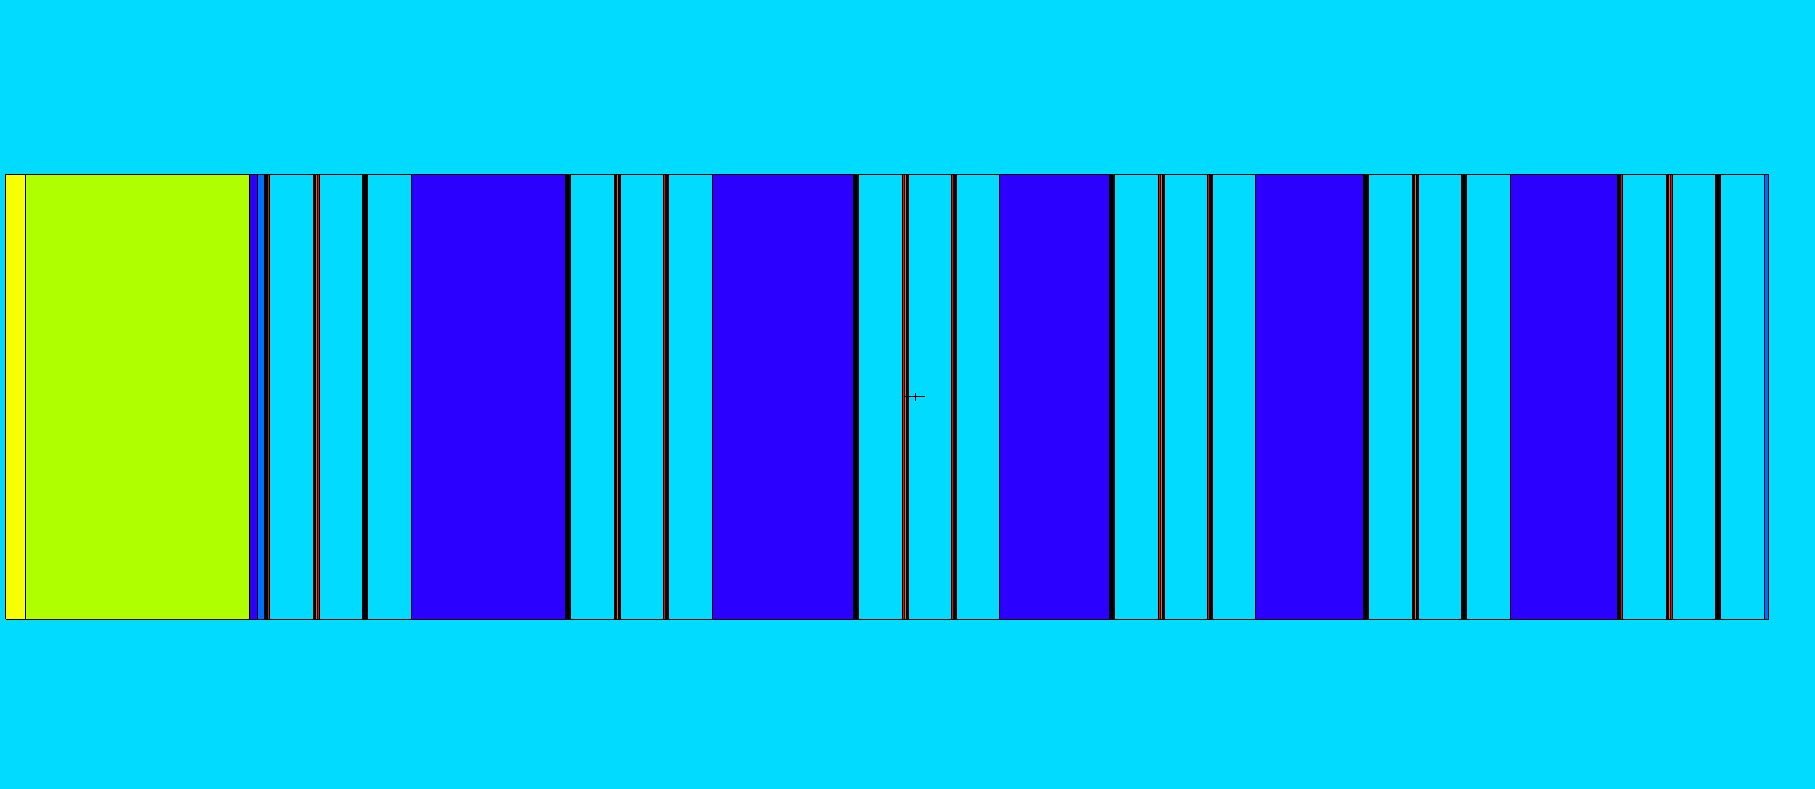
\includegraphics[trim = 0mm 0mm 2mm 0mm, clip,width=0.75\columnwidth]{./figures/ipf_stack_nolabels.PNG}
 % mcnp_vised2.PNG.png: 688x443 pixel, 96dpi, 18.21x11.72 cm, bb=0 0 516 332
 \caption{Blah blah blah
%  MCNP6 model of the HFNG target chamber, with reference scale. The co-loaded foils can be seen in the target chamber center.  The ovals indicate the location of water cooling channels.
}
 \label{fig:ipf_vised}
\end{figure}





\begin{figure*}
    \centering    
    \subfloat{
        \centering
%         \includegraphics[width=\textwidth]{./figures/target2.png}
        \subfigimg[width=0.497\textwidth]{a)}{./figures/Al_ntallies.pdf}{50}
%         \caption{Decay curve for the $\beta^-$ decay of \ce{^{116}In}.}
        %         \refstepcounter{subfigure}
%          \label{fig:91mNb}
%    }
%      \subfloat{
%         \centering
%         \includegraphics[width=\columnwidth]{./figures/Capture.PNG}
        \subfigimg[width=0.497\textwidth]{b)}{./figures/Cu_ntallies.pdf}{50}
%         \caption{ Decay curve for the $\beta^+$ decay of \ce{^{64}Cu}.}
%         \refstepcounter{subfigure} 
%         \label{fig:92mNb}
   \hspace{-10pt}}%
    \\
    \subfloat{
        \centering
%         \includegraphics[width=\columnwidth]{./figures/Capture.PNG}
        \subfigimg[width=0.497\textwidth]{c)}{./figures/Nb_ntallies.pdf}{50}
%         \caption{ Decay curve for the isomeric transition of \ce{^{115m}In}.}
%         \refstepcounter{subfigure}
%          \label{fig:93mMo}
   }%
    \caption{Decay curves used to verify photopeak transition assignment. (a) Decay curve for the isomeric transition of \ce{^{115m}In}, (b) decay curve for the isomeric transition of \ce{^{113m}In}, and (c) decay curve for the $\beta^-$ decay of \ce{^{116}In}.}
%      \phantomcaption{}
     \label{fig:ipf_ntallies}
\end{figure*}


\begin{figure*}
    \centering    
    \subfloat{
        \centering
%         \includegraphics[width=\textwidth]{./figures/target2.png}
        \subfigimg[width=0.495\textwidth]{a)}{./figures/Al_ptallies.pdf}{80}
%         \caption{Decay curve for the $\beta^-$ decay of \ce{^{116}In}.}
        %         \refstepcounter{subfigure}
%          \label{fig:91mNb}
%    }
%      \subfloat{
%         \centering
%         \includegraphics[width=\columnwidth]{./figures/Capture.PNG}
        \subfigimg[width=0.495\textwidth]{b)}{./figures/Cu_ptallies.pdf}{80}
%         \caption{ Decay curve for the $\beta^+$ decay of \ce{^{64}Cu}.}
%         \refstepcounter{subfigure} 
%         \label{fig:92mNb}
   \hspace{-10pt}}%
    \caption{Decay curves used to verify photopeak transition assignment. (a) Decay curve for the isomeric transition of \ce{^{115m}In}, (b) decay curve for the isomeric transition of \ce{^{113m}In}, and (c) decay curve for the $\beta^-$ decay of \ce{^{116}In}.}
%      \phantomcaption{}
     \label{fig:ipf_ptallies_appendix}
\end{figure*}



\begin{figure}
 \centering
%                                l   b      r    top
%  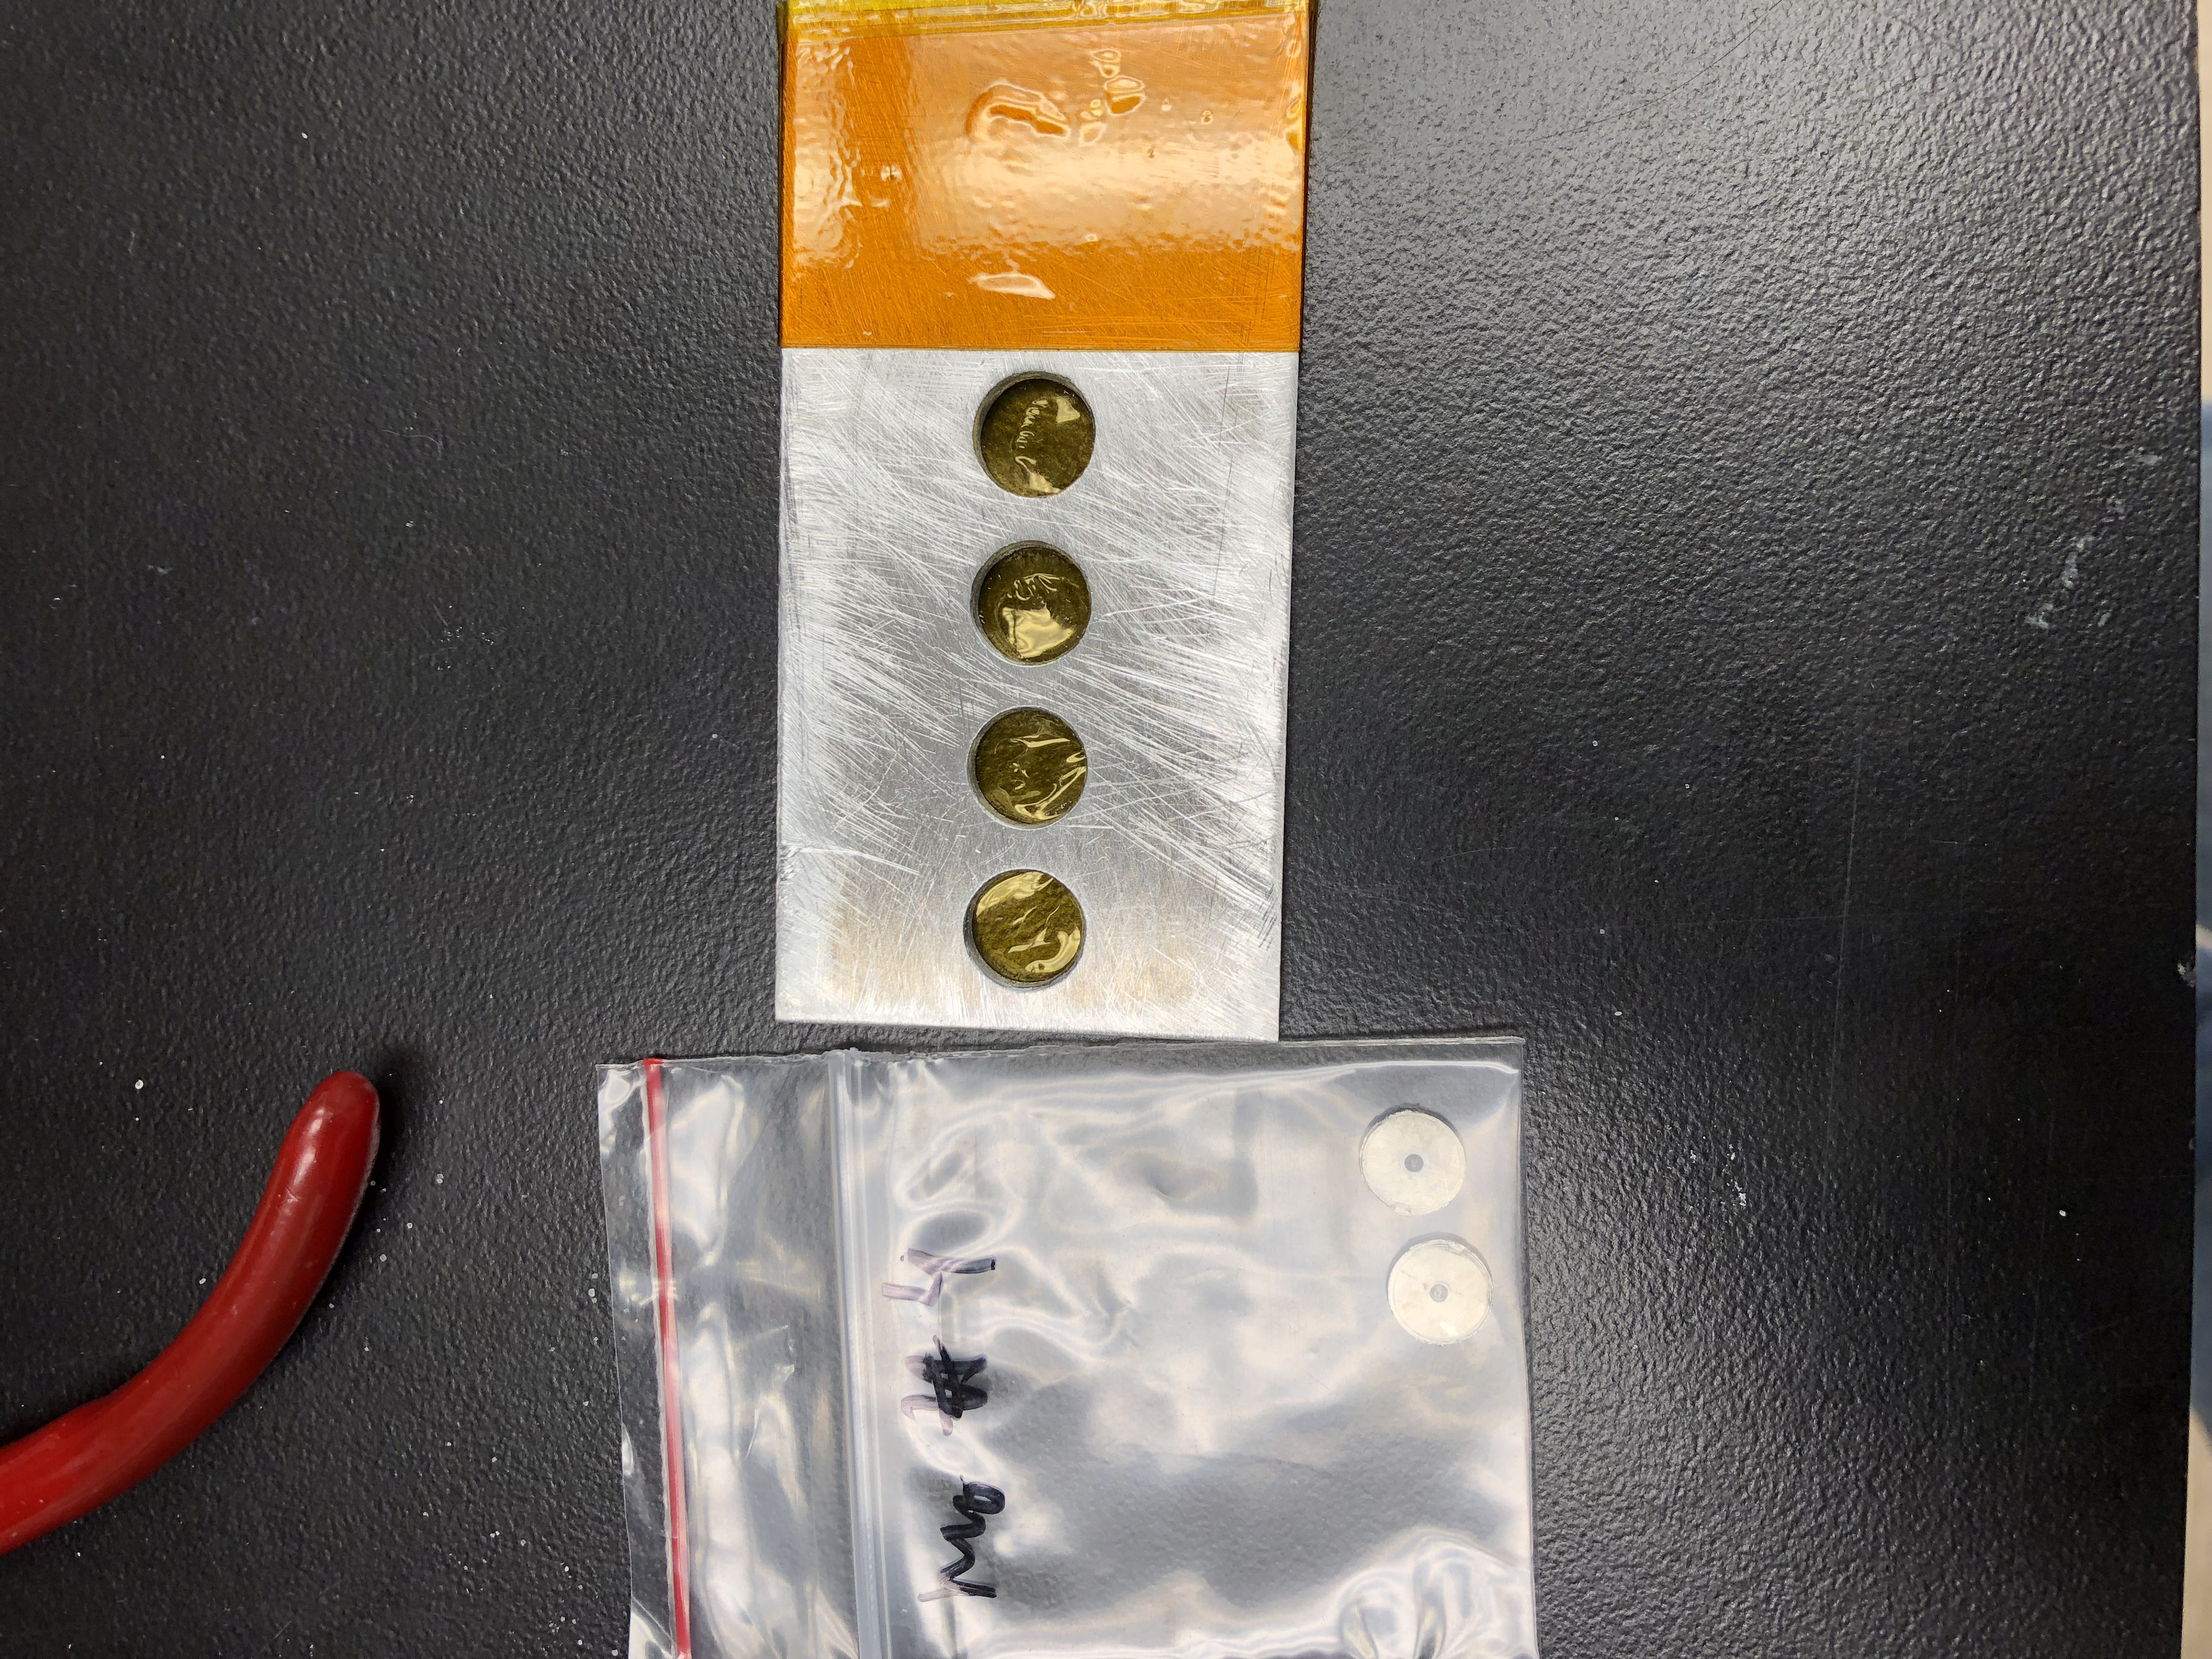
\includegraphics[clip=true,trim=5pt 1000pt 10pt 900pt,width=0.75\columnwidth,angle=90]{./figures/IMG_8840.JPG}
%  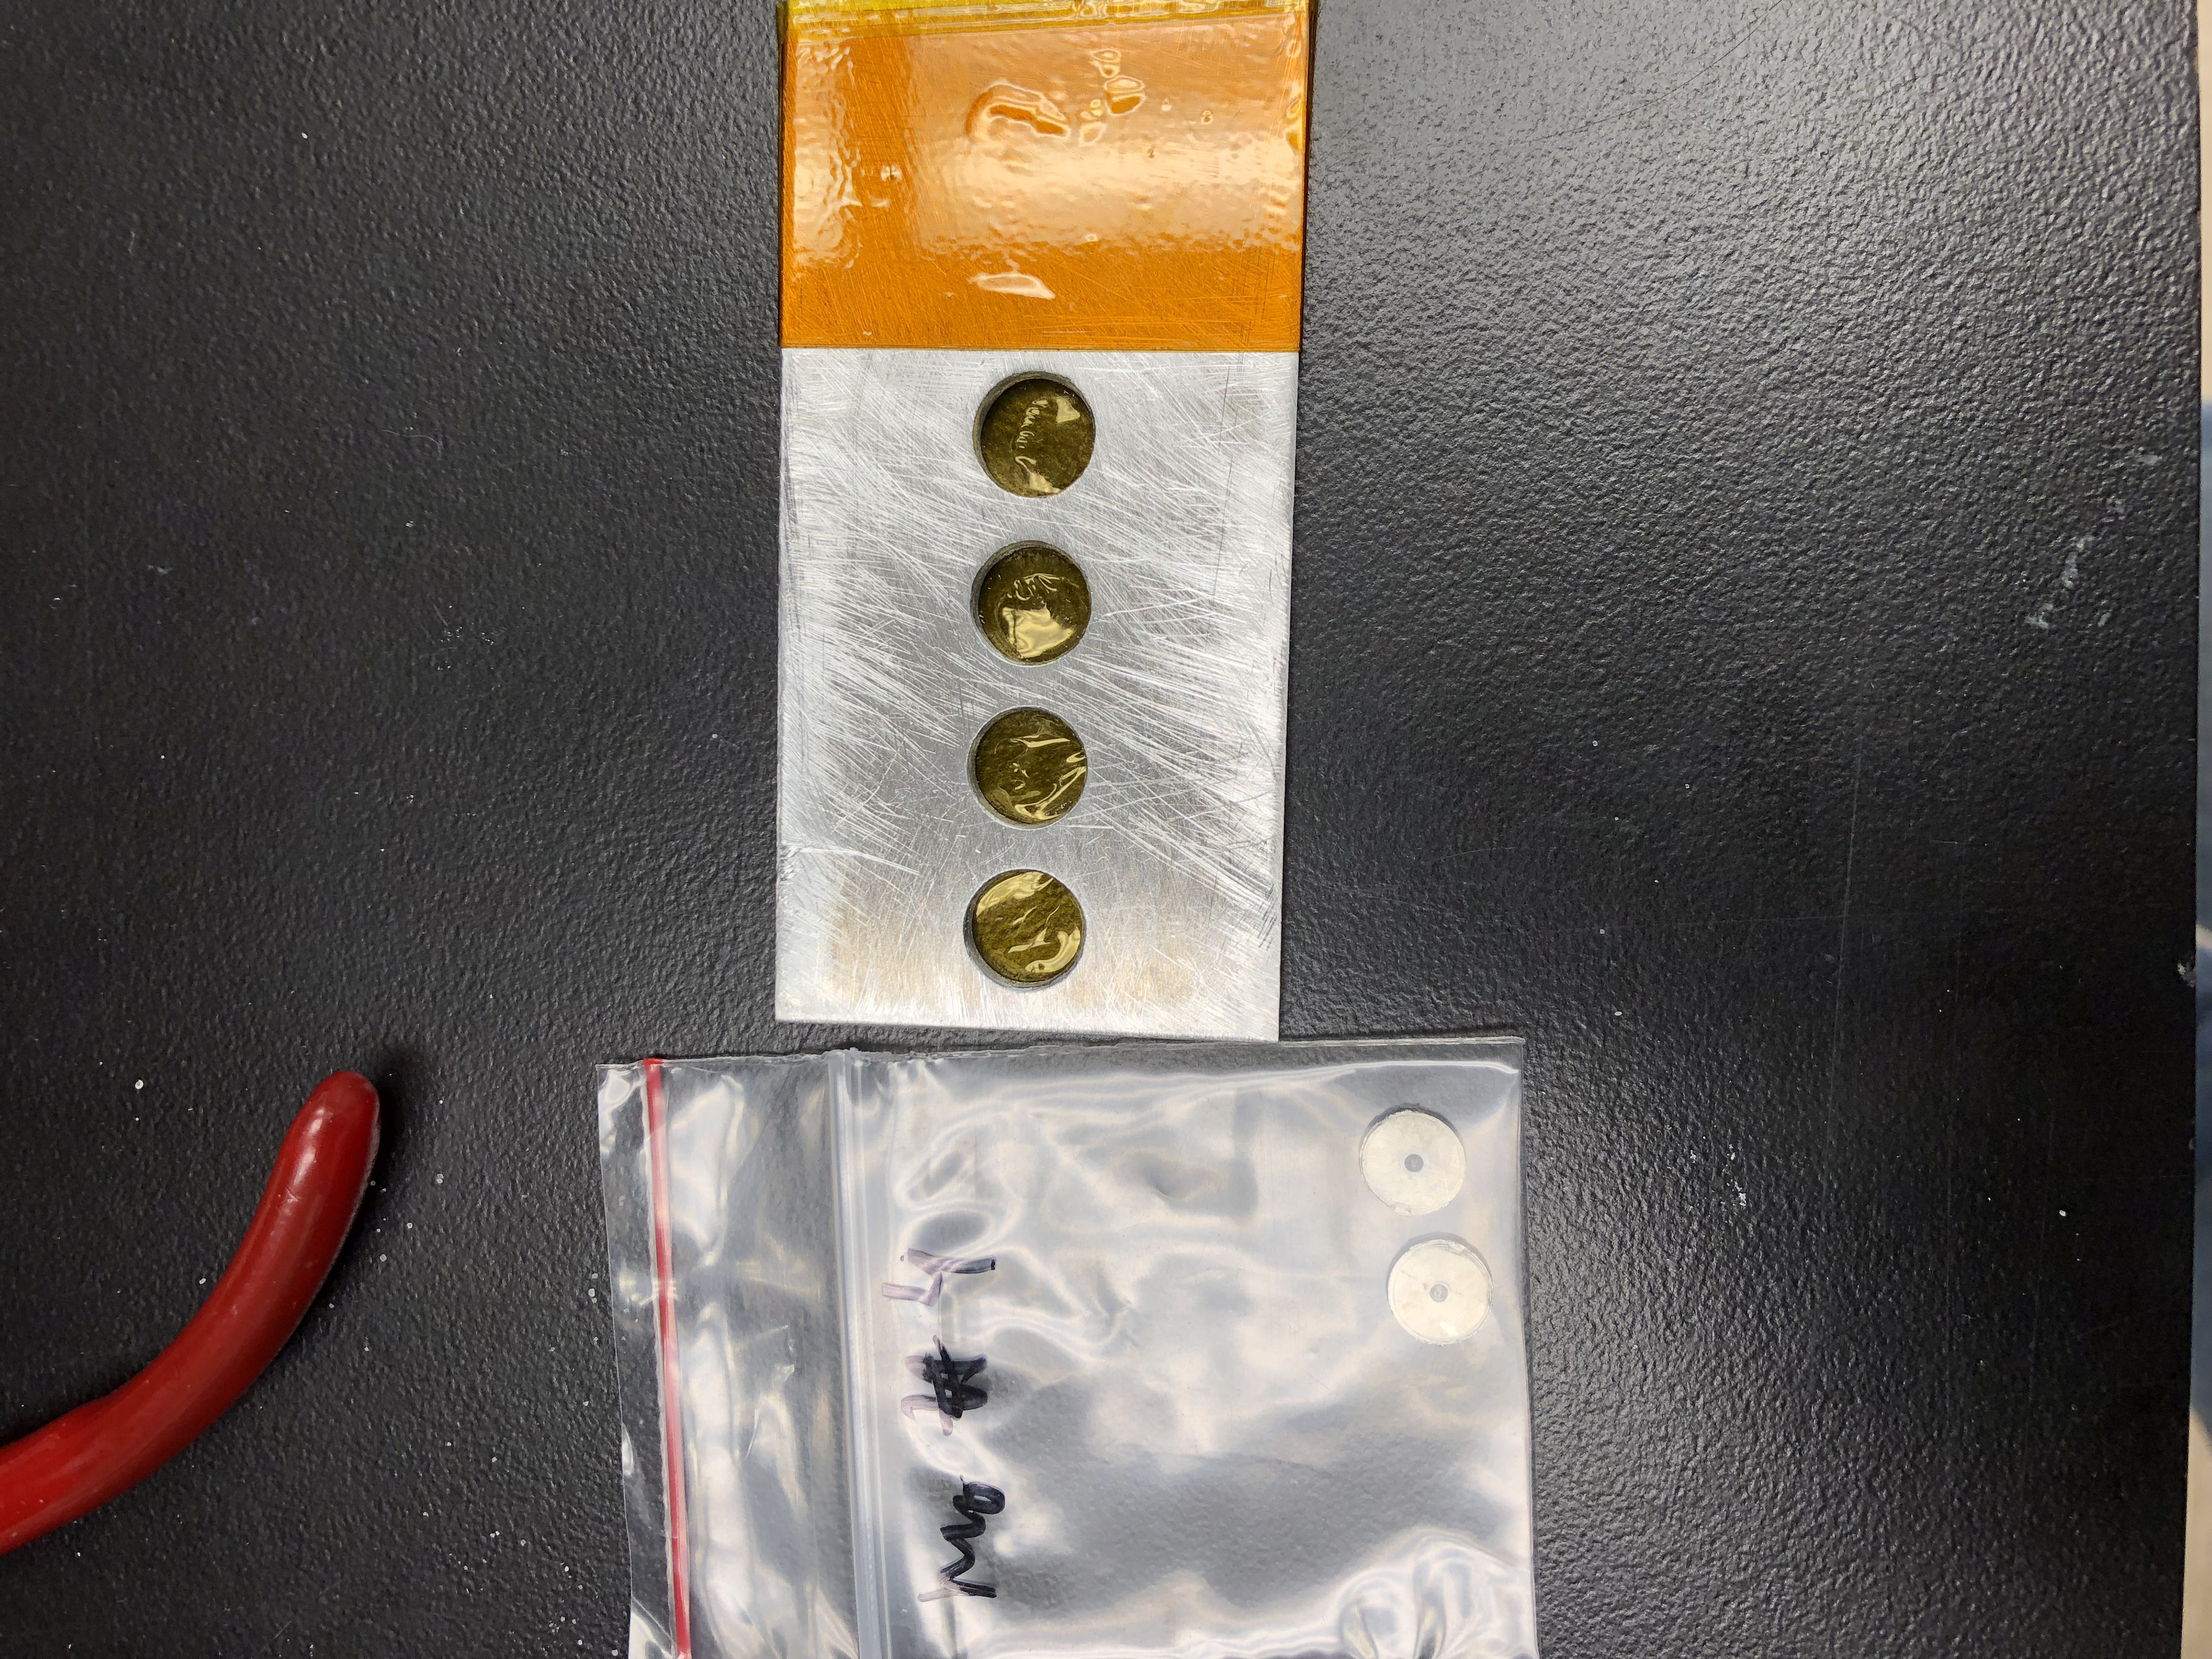
\includegraphics[width=0.75\columnwidth,angle=270]{./figures/IMG_8840.JPG}
 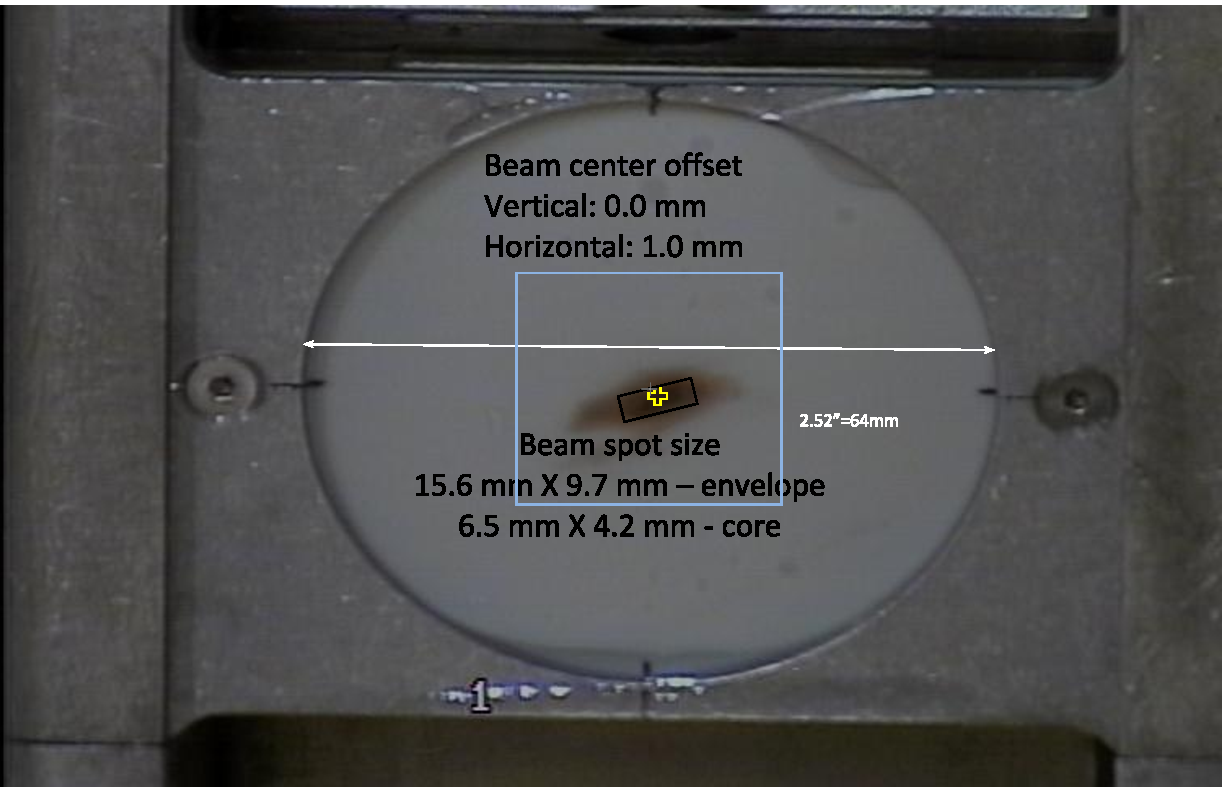
\includegraphics[width=0.75\columnwidth]{./figures/ipf_preexp_beam_spot-cropped.pdf}
 % IMG_8840.JPG: 4032x3024 pixel, 72dpi, 142.24x106.68 cm, bb=0 0 4032 3024
 \caption{ipf preexp beam spot.}
 \label{fig:ipf_preexp_beam_spot}
\end{figure}


\begin{figure}
 \centering
%                                l   b      r    top
%  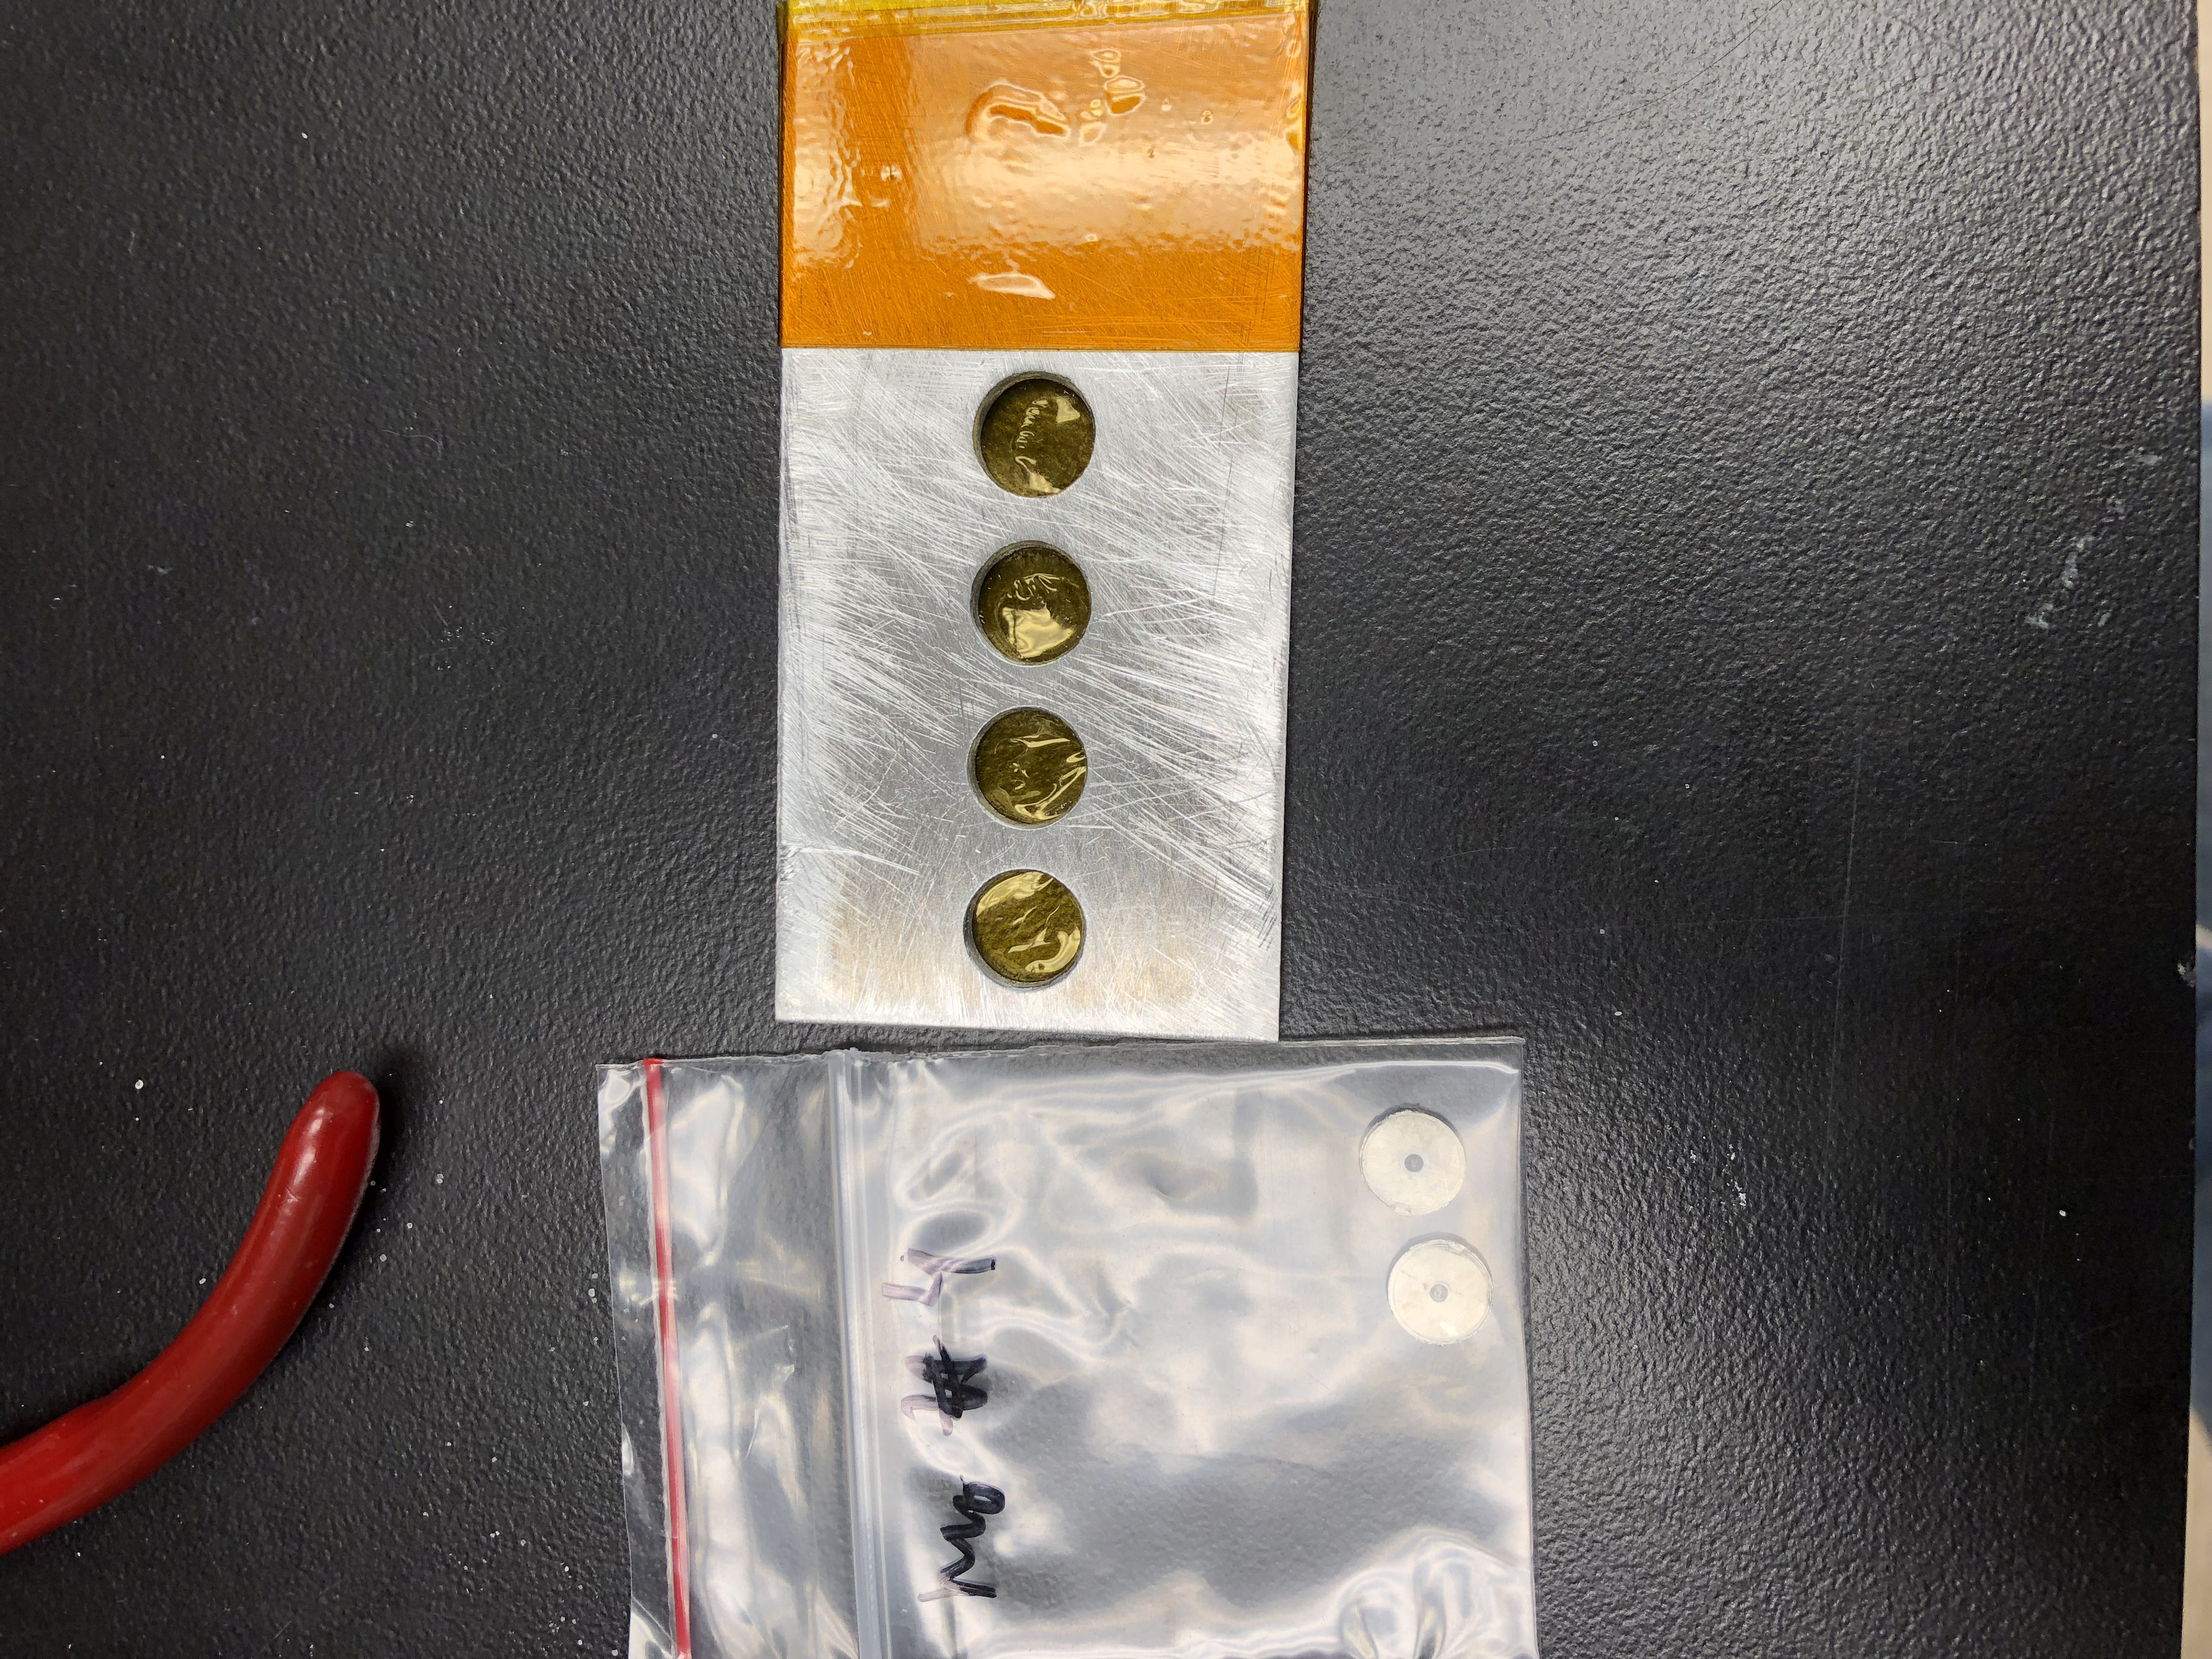
\includegraphics[clip=true,trim=5pt 1000pt 10pt 900pt,width=0.75\columnwidth,angle=90]{./figures/IMG_8840.JPG}
%  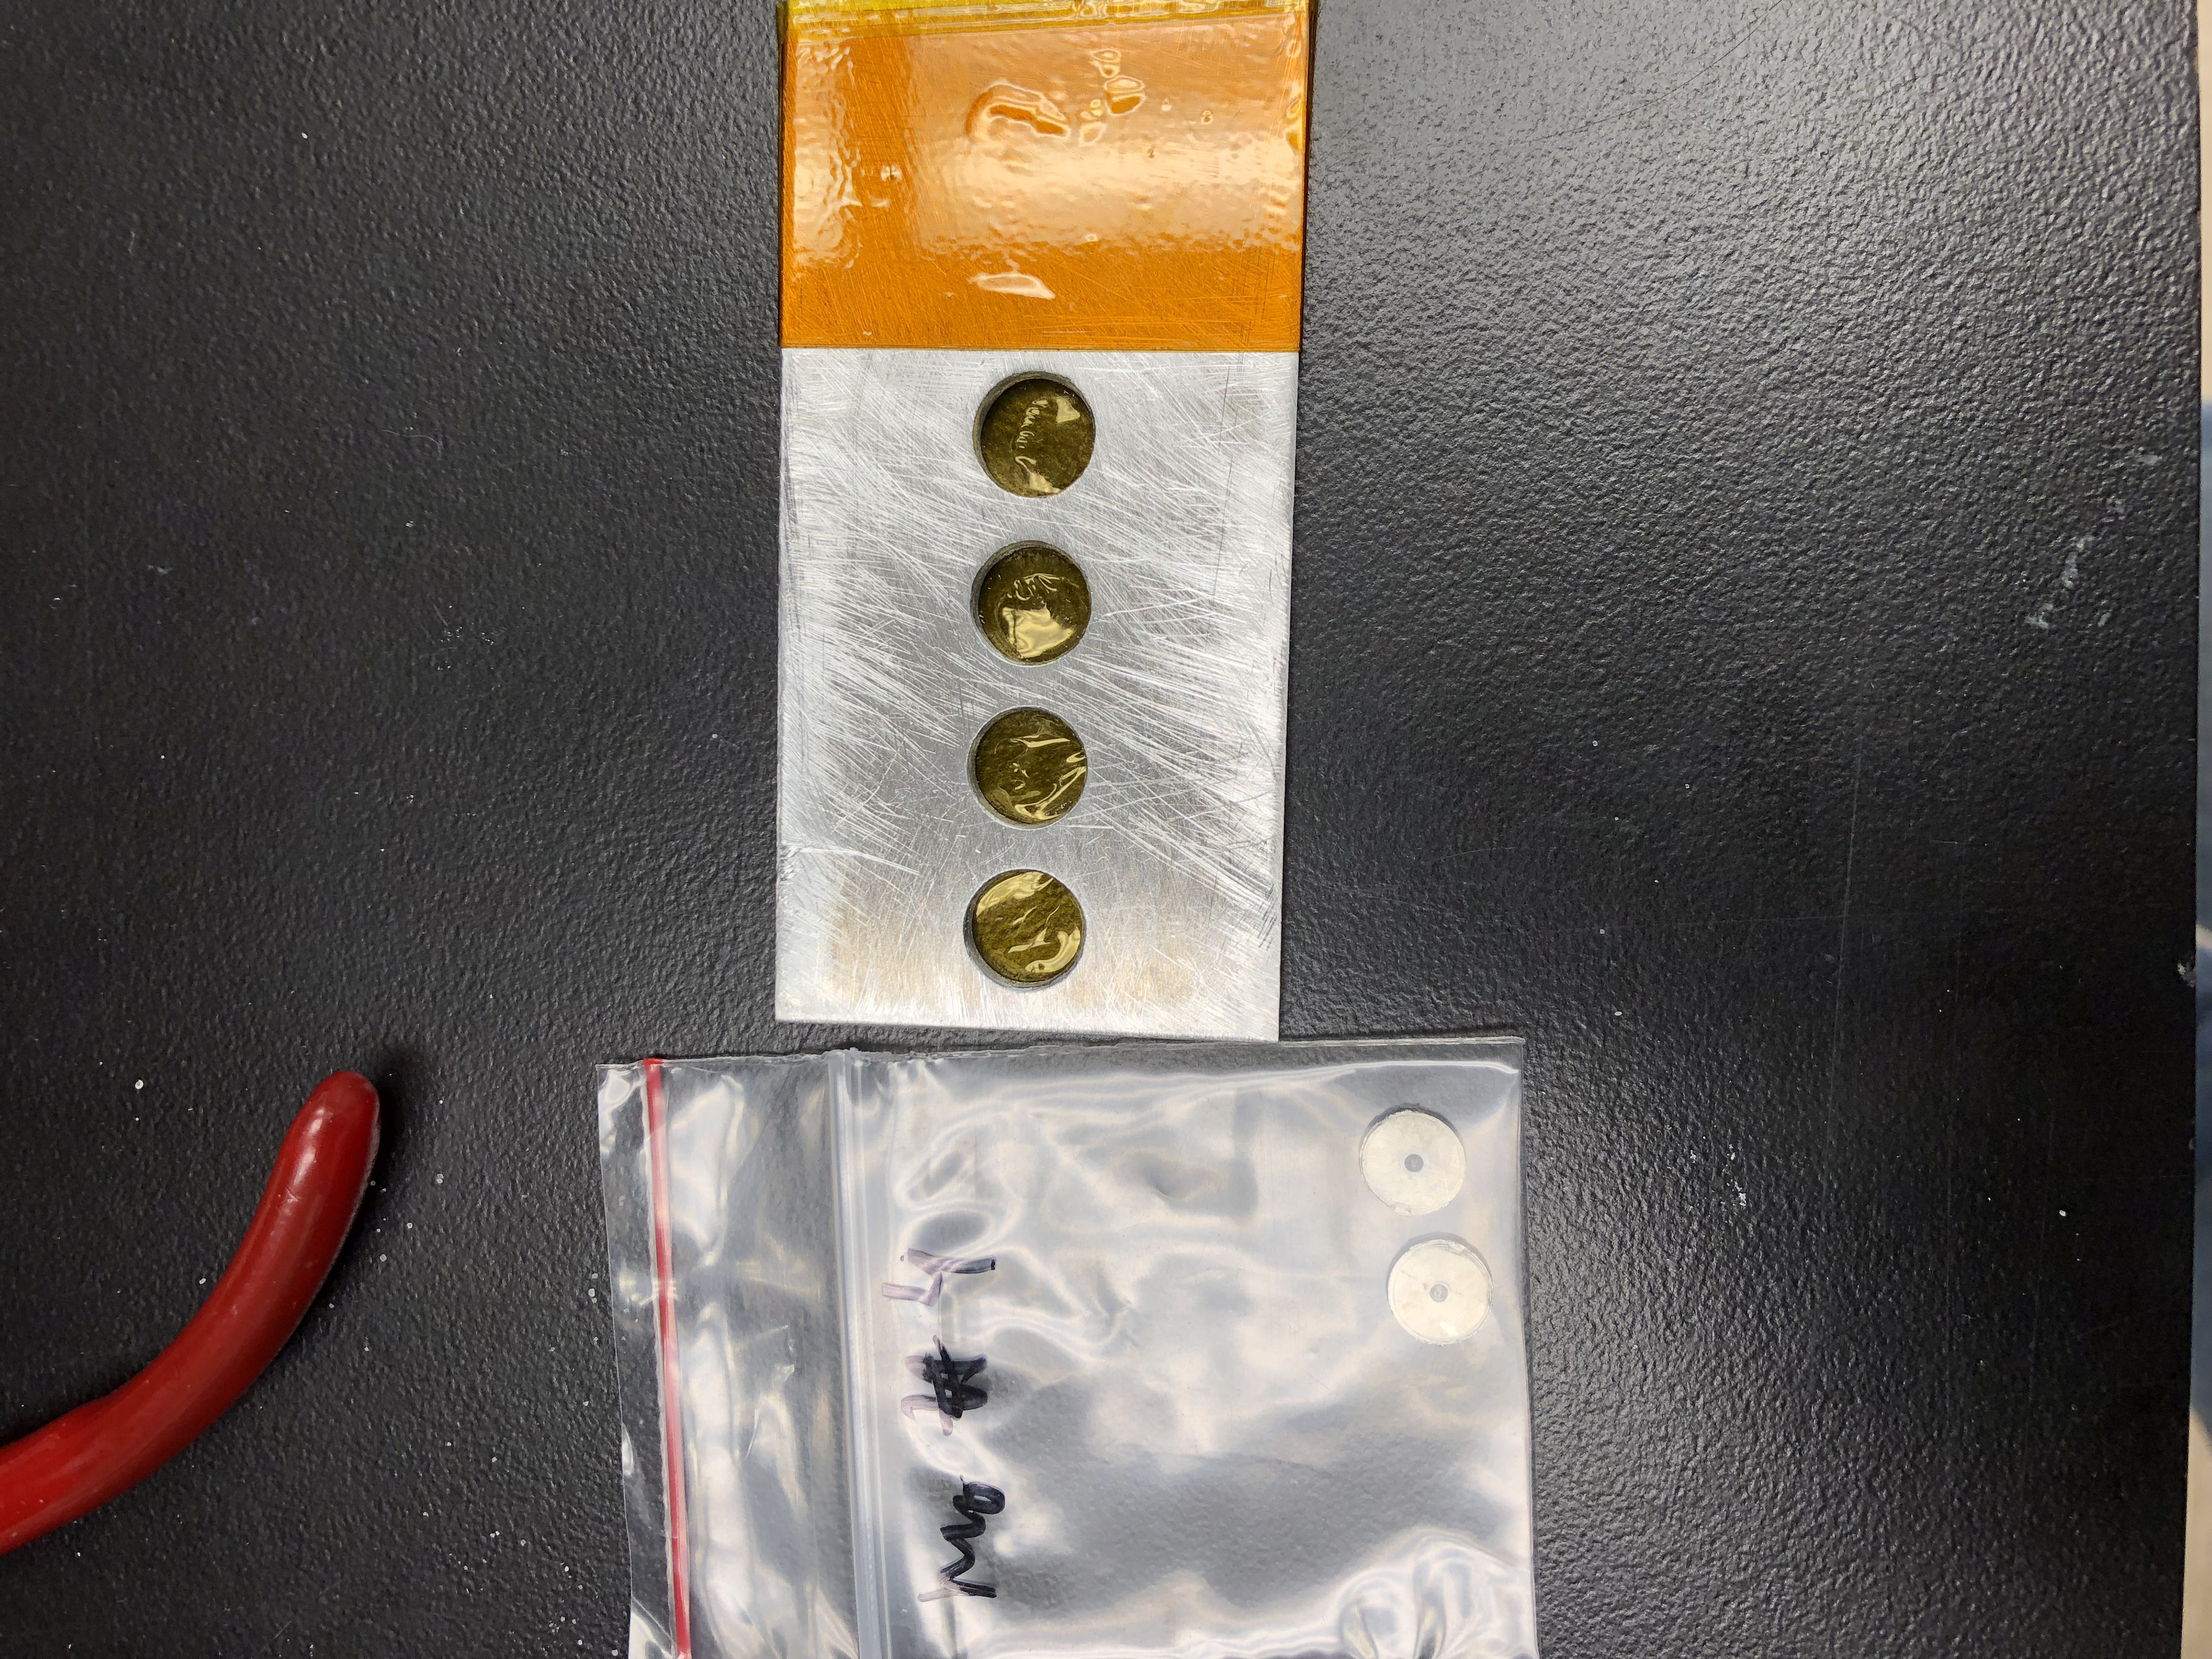
\includegraphics[width=0.75\columnwidth,angle=270]{./figures/IMG_8840.JPG}
 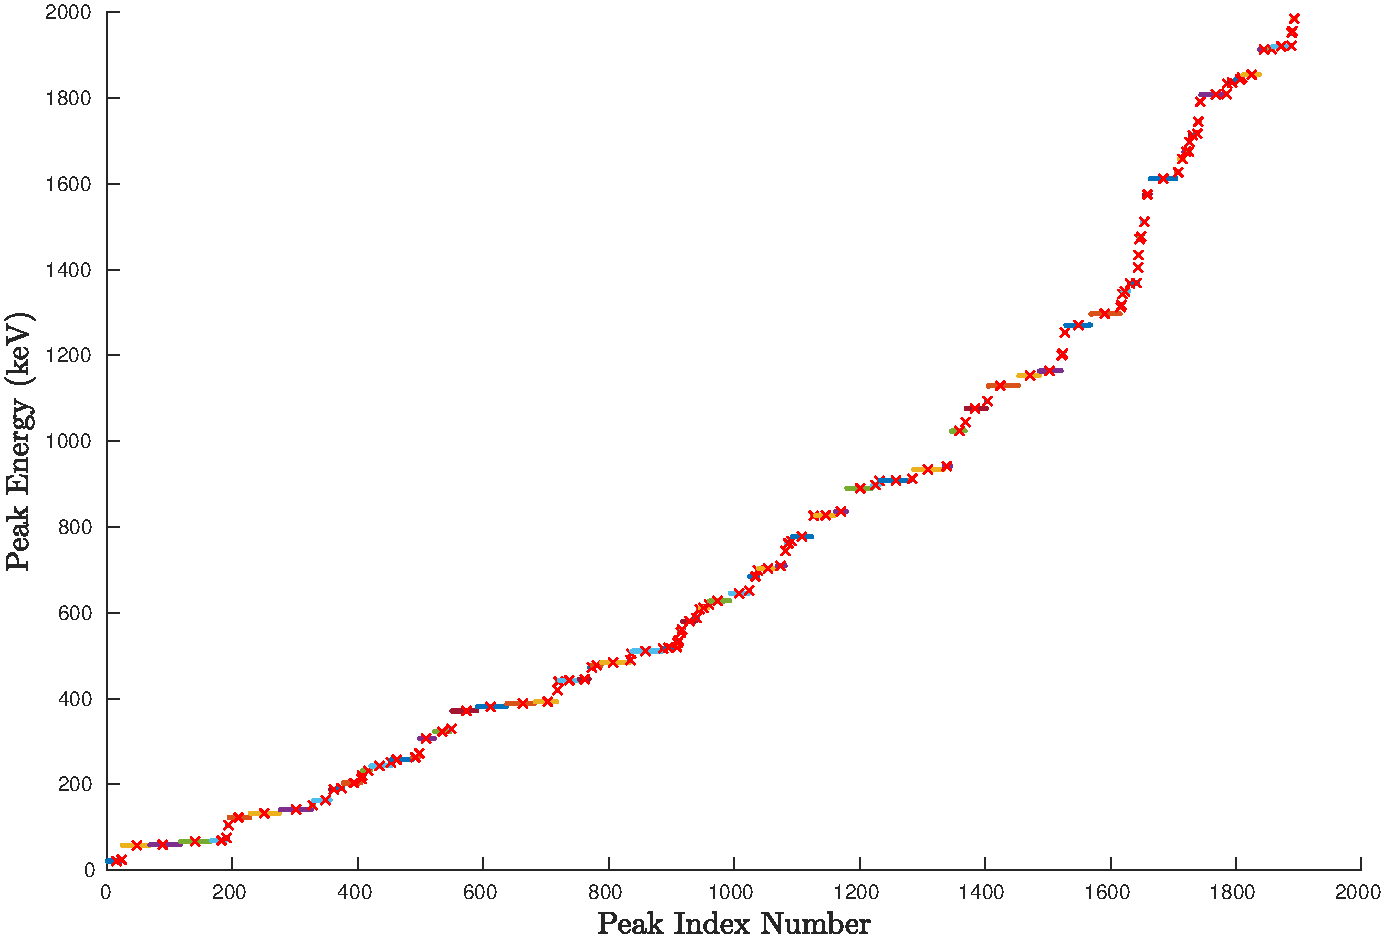
\includegraphics[width=0.75\columnwidth]{./figures/peak_stairsteps.pdf}
 % IMG_8840.JPG: 4032x3024 pixel, 72dpi, 142.24x106.68 cm, bb=0 0 4032 3024
 \caption{peak stairsteps.}
 \label{fig:peak_stairsteps}
\end{figure}



\begin{figure}
 \centering
%                                l   b      r    top
%  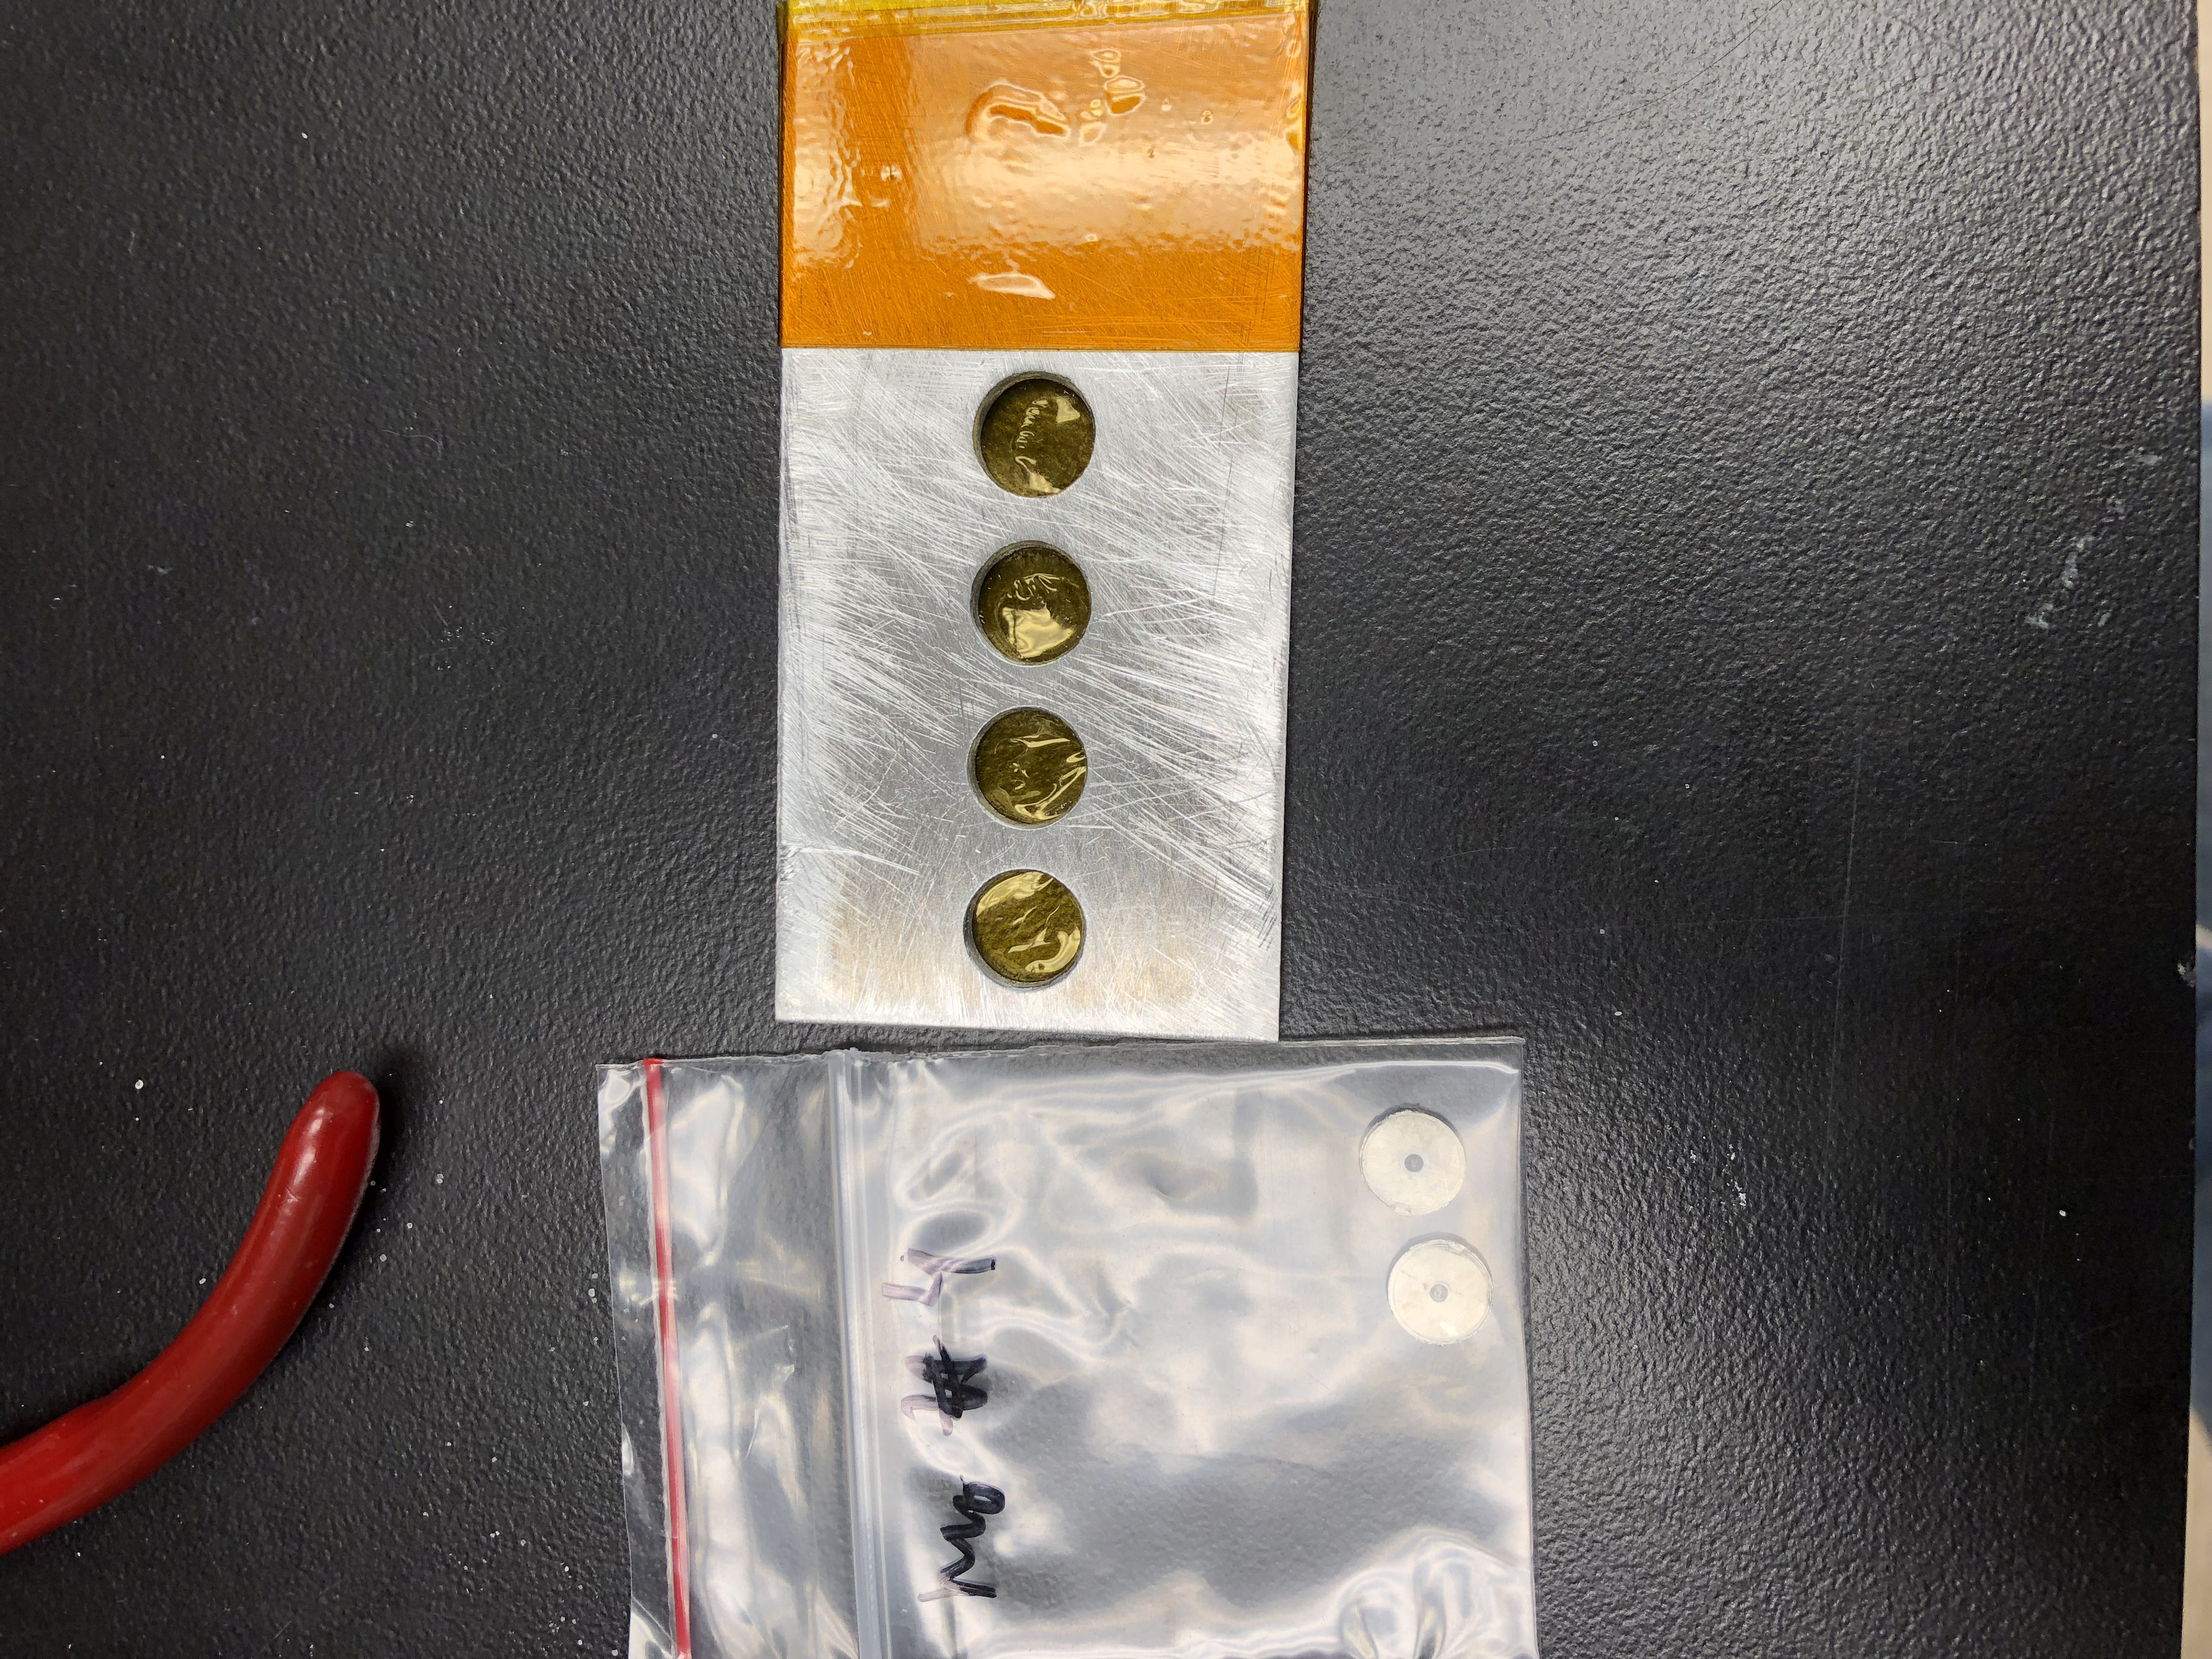
\includegraphics[clip=true,trim=5pt 1000pt 10pt 900pt,width=0.75\columnwidth,angle=90]{./figures/IMG_8840.JPG}
%  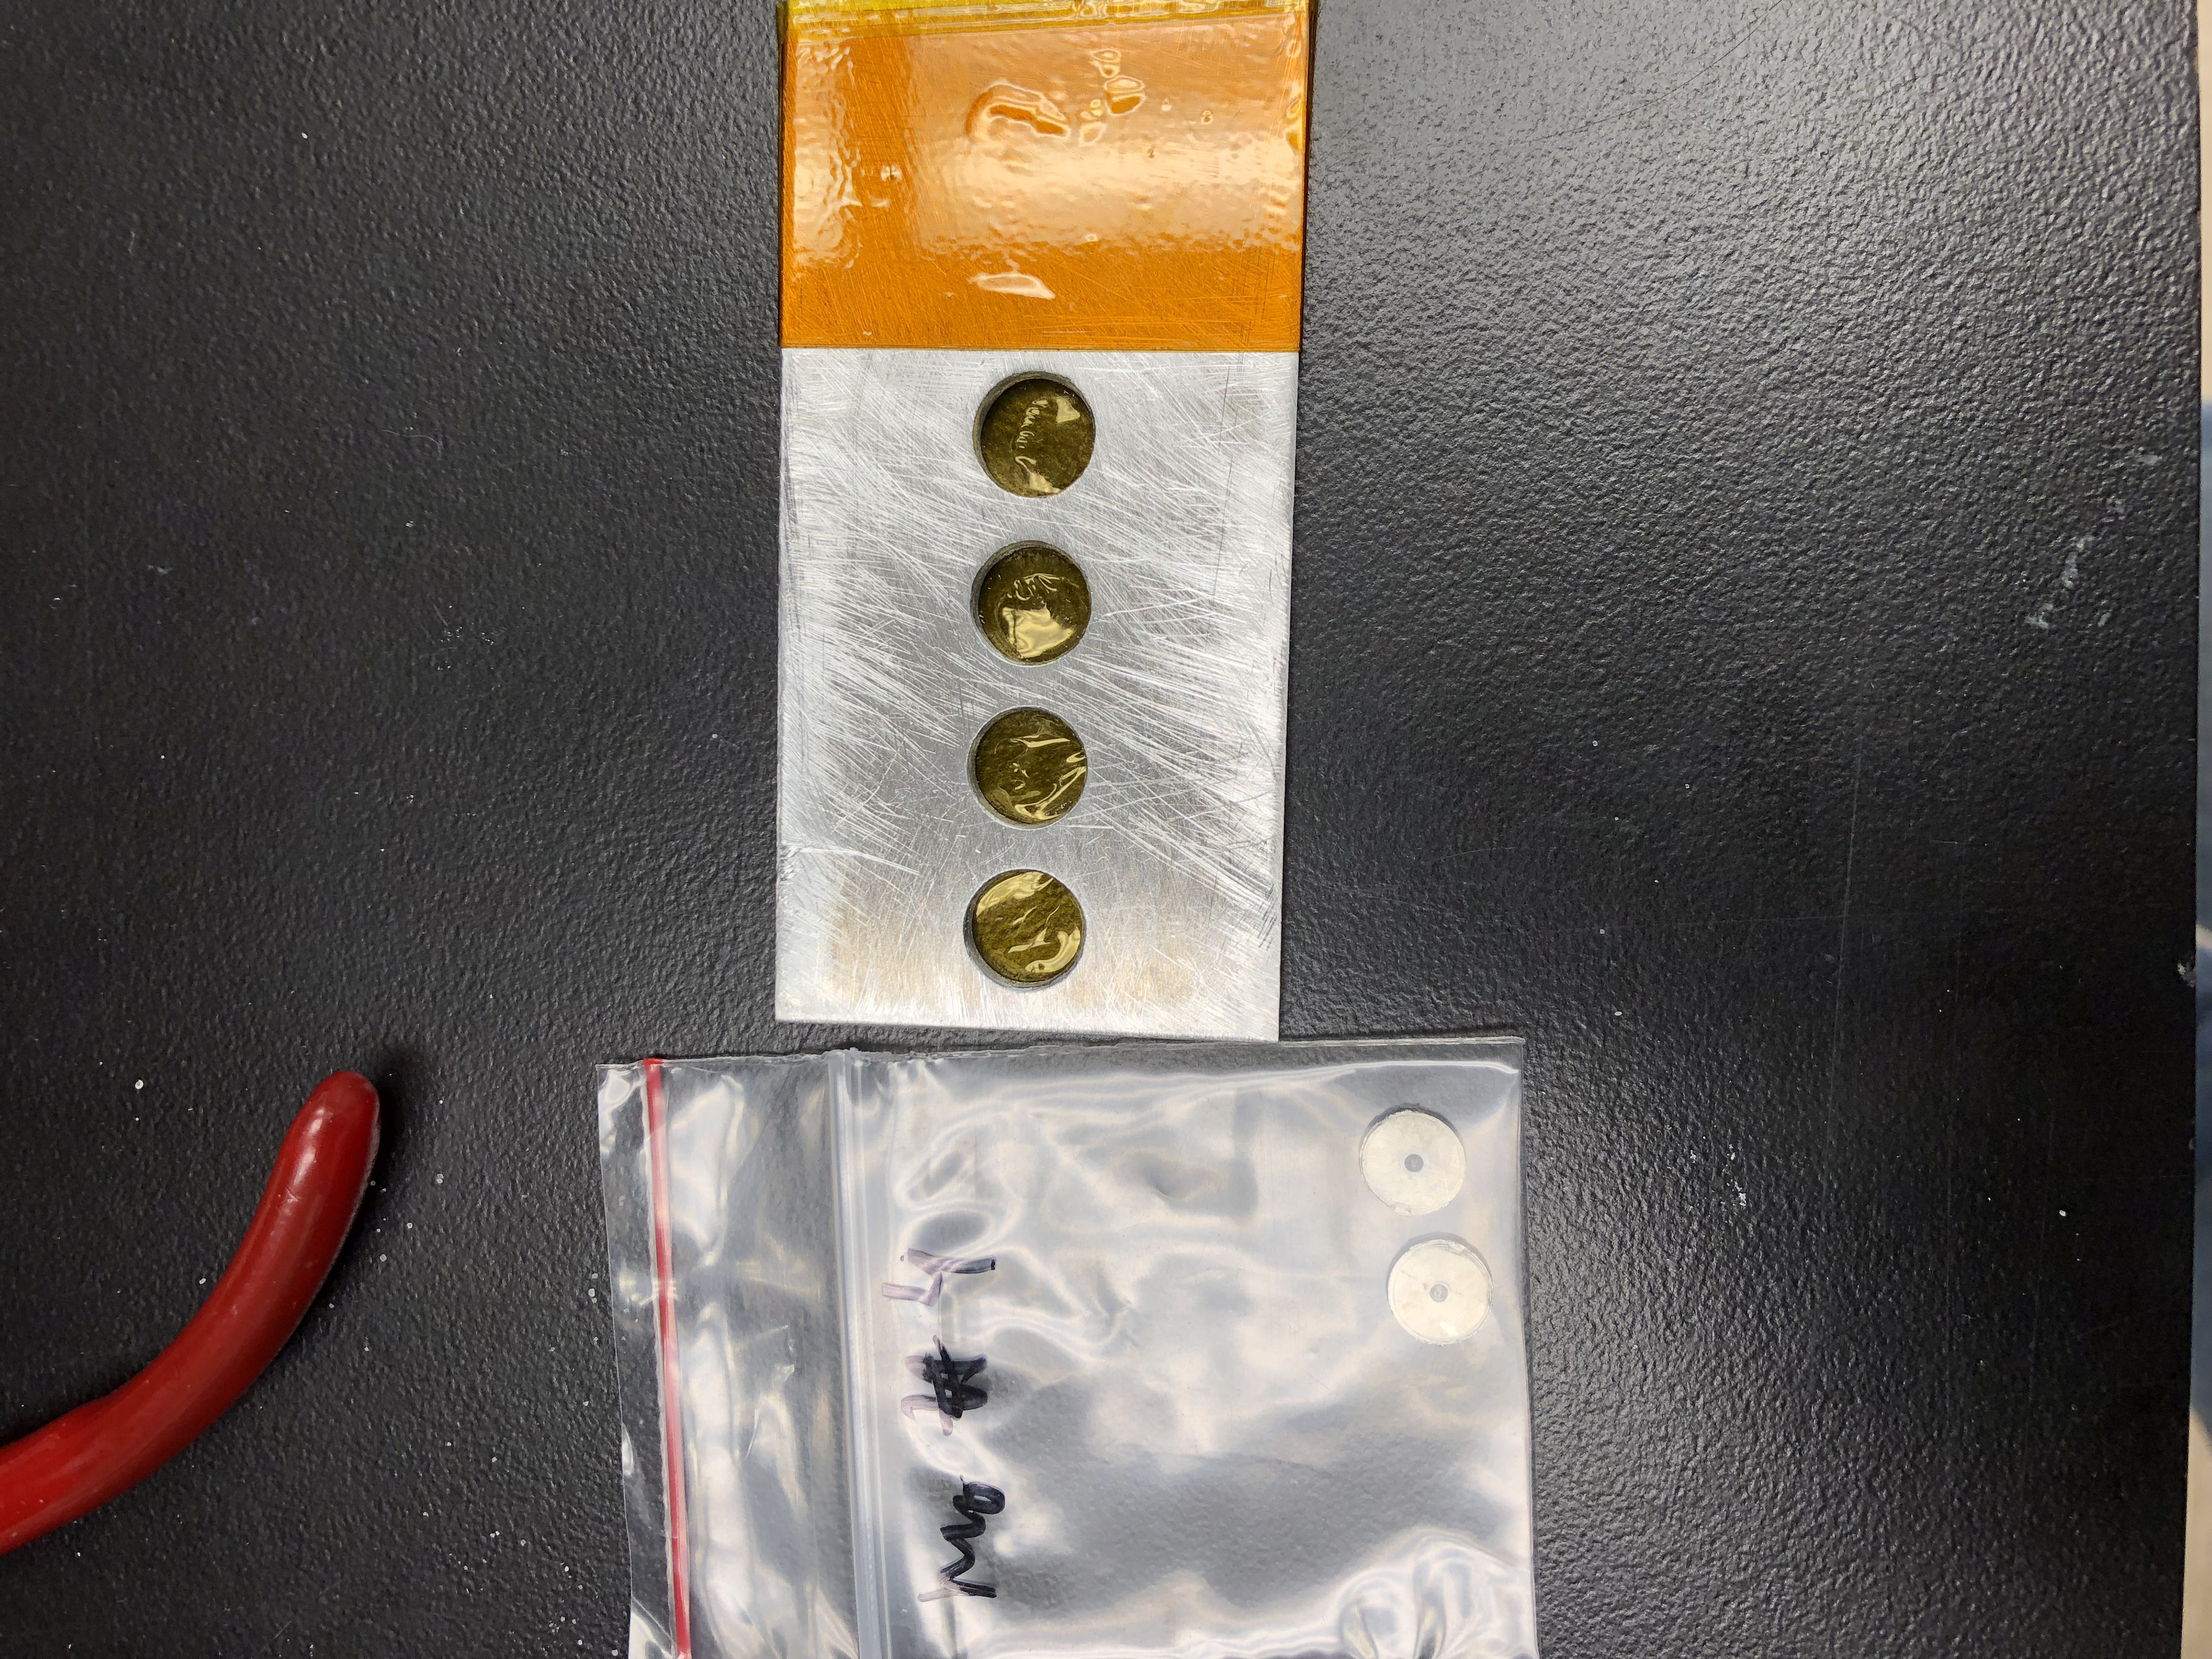
\includegraphics[width=0.75\columnwidth,angle=270]{./figures/IMG_8840.JPG}
 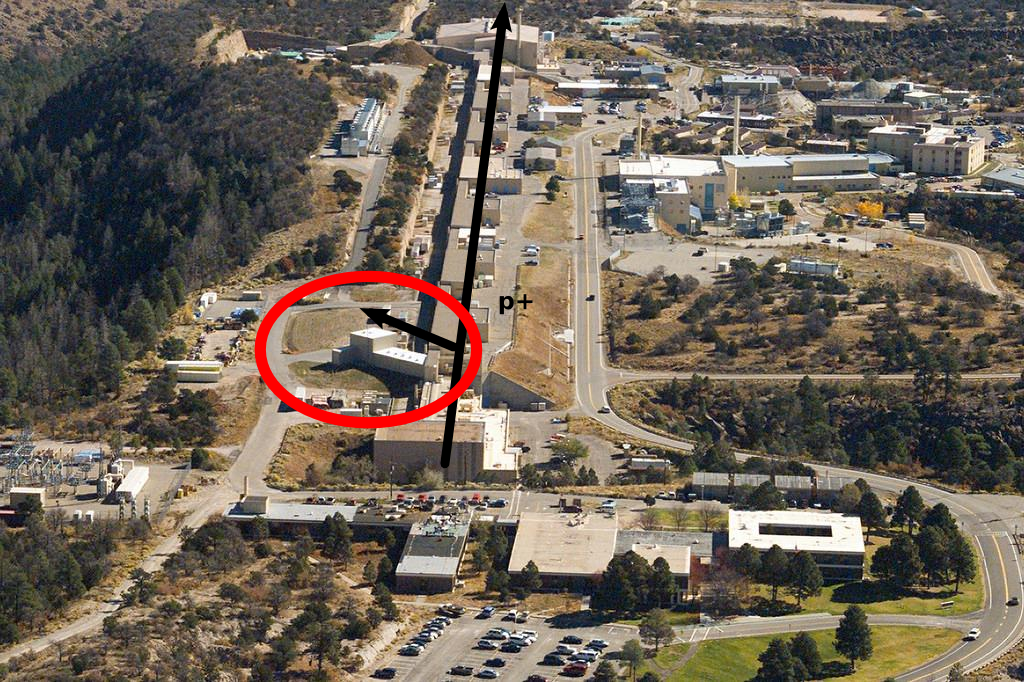
\includegraphics[width=0.75\columnwidth]{./figures/ipf_beamline_alternate.png}
 % IMG_8840.JPG: 4032x3024 pixel, 72dpi, 142.24x106.68 cm, bb=0 0 4032 3024
 \caption{the 977858699167c3aeabdb.}
 \label{fig:ipf_beamline_alternate}
\end{figure}


\begin{figure}
 \centering
%                                l   b      r    top
%  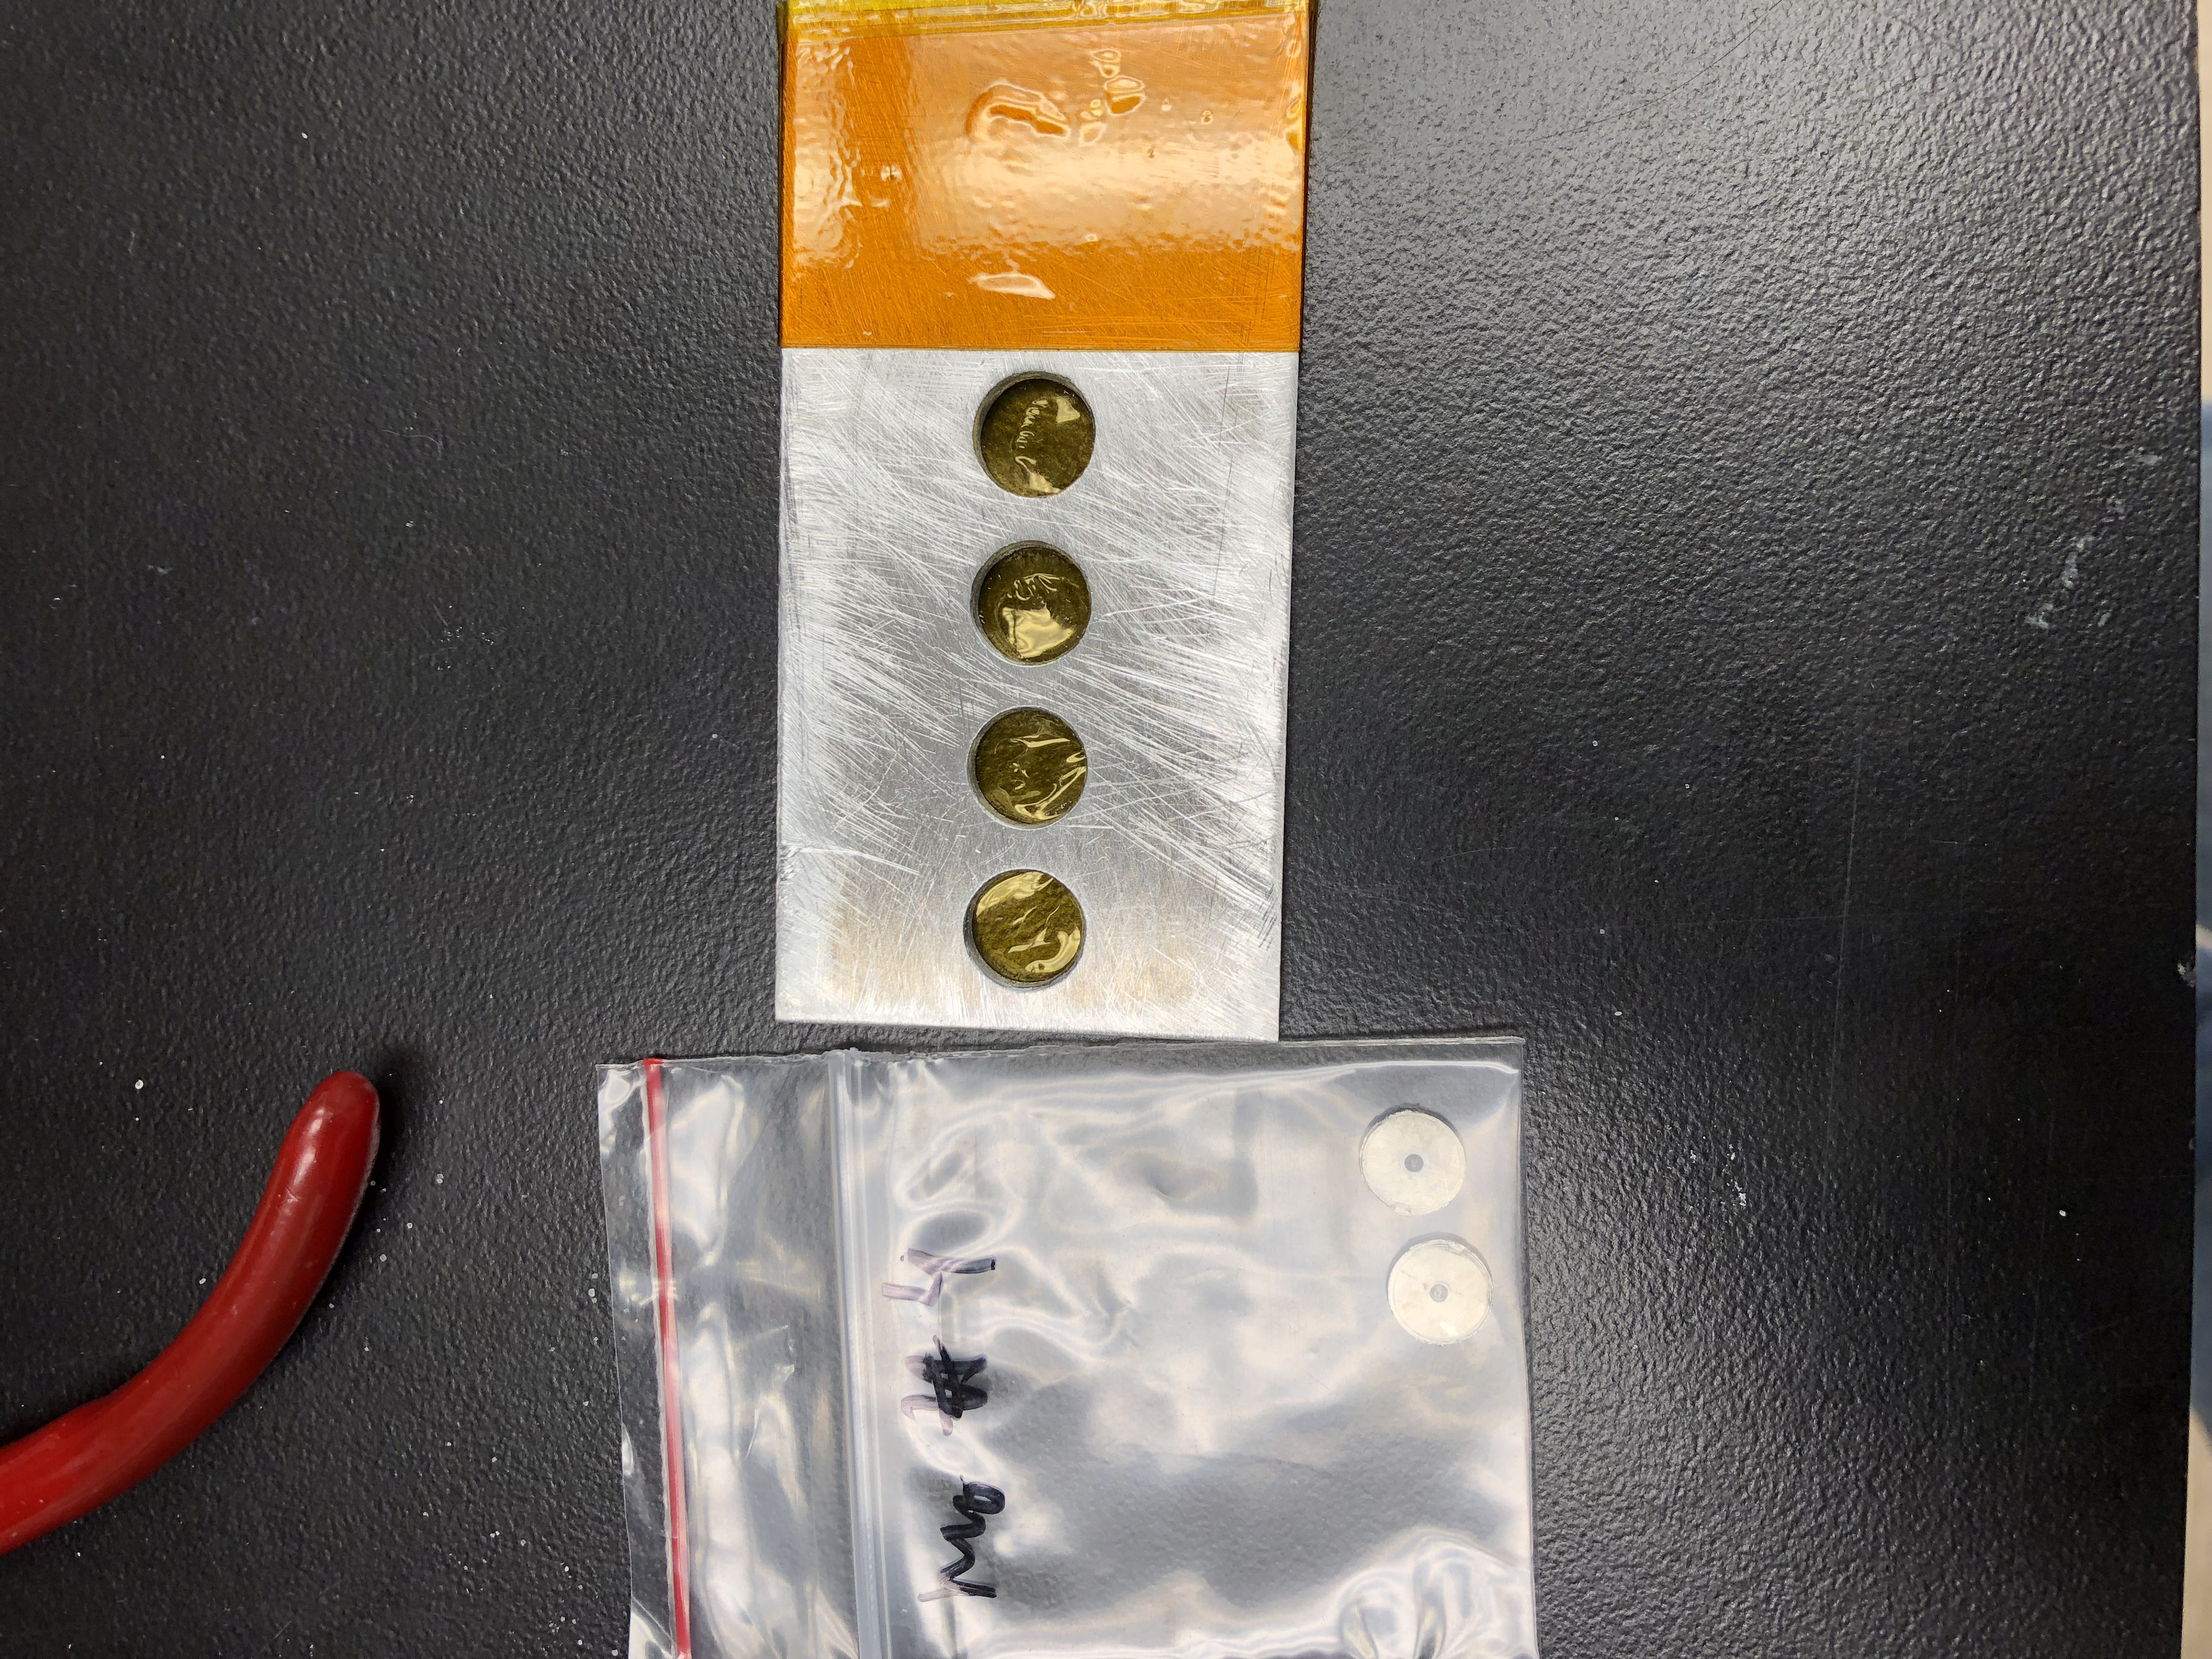
\includegraphics[clip=true,trim=5pt 1000pt 10pt 900pt,width=0.75\columnwidth,angle=90]{./figures/IMG_8840.JPG}
%  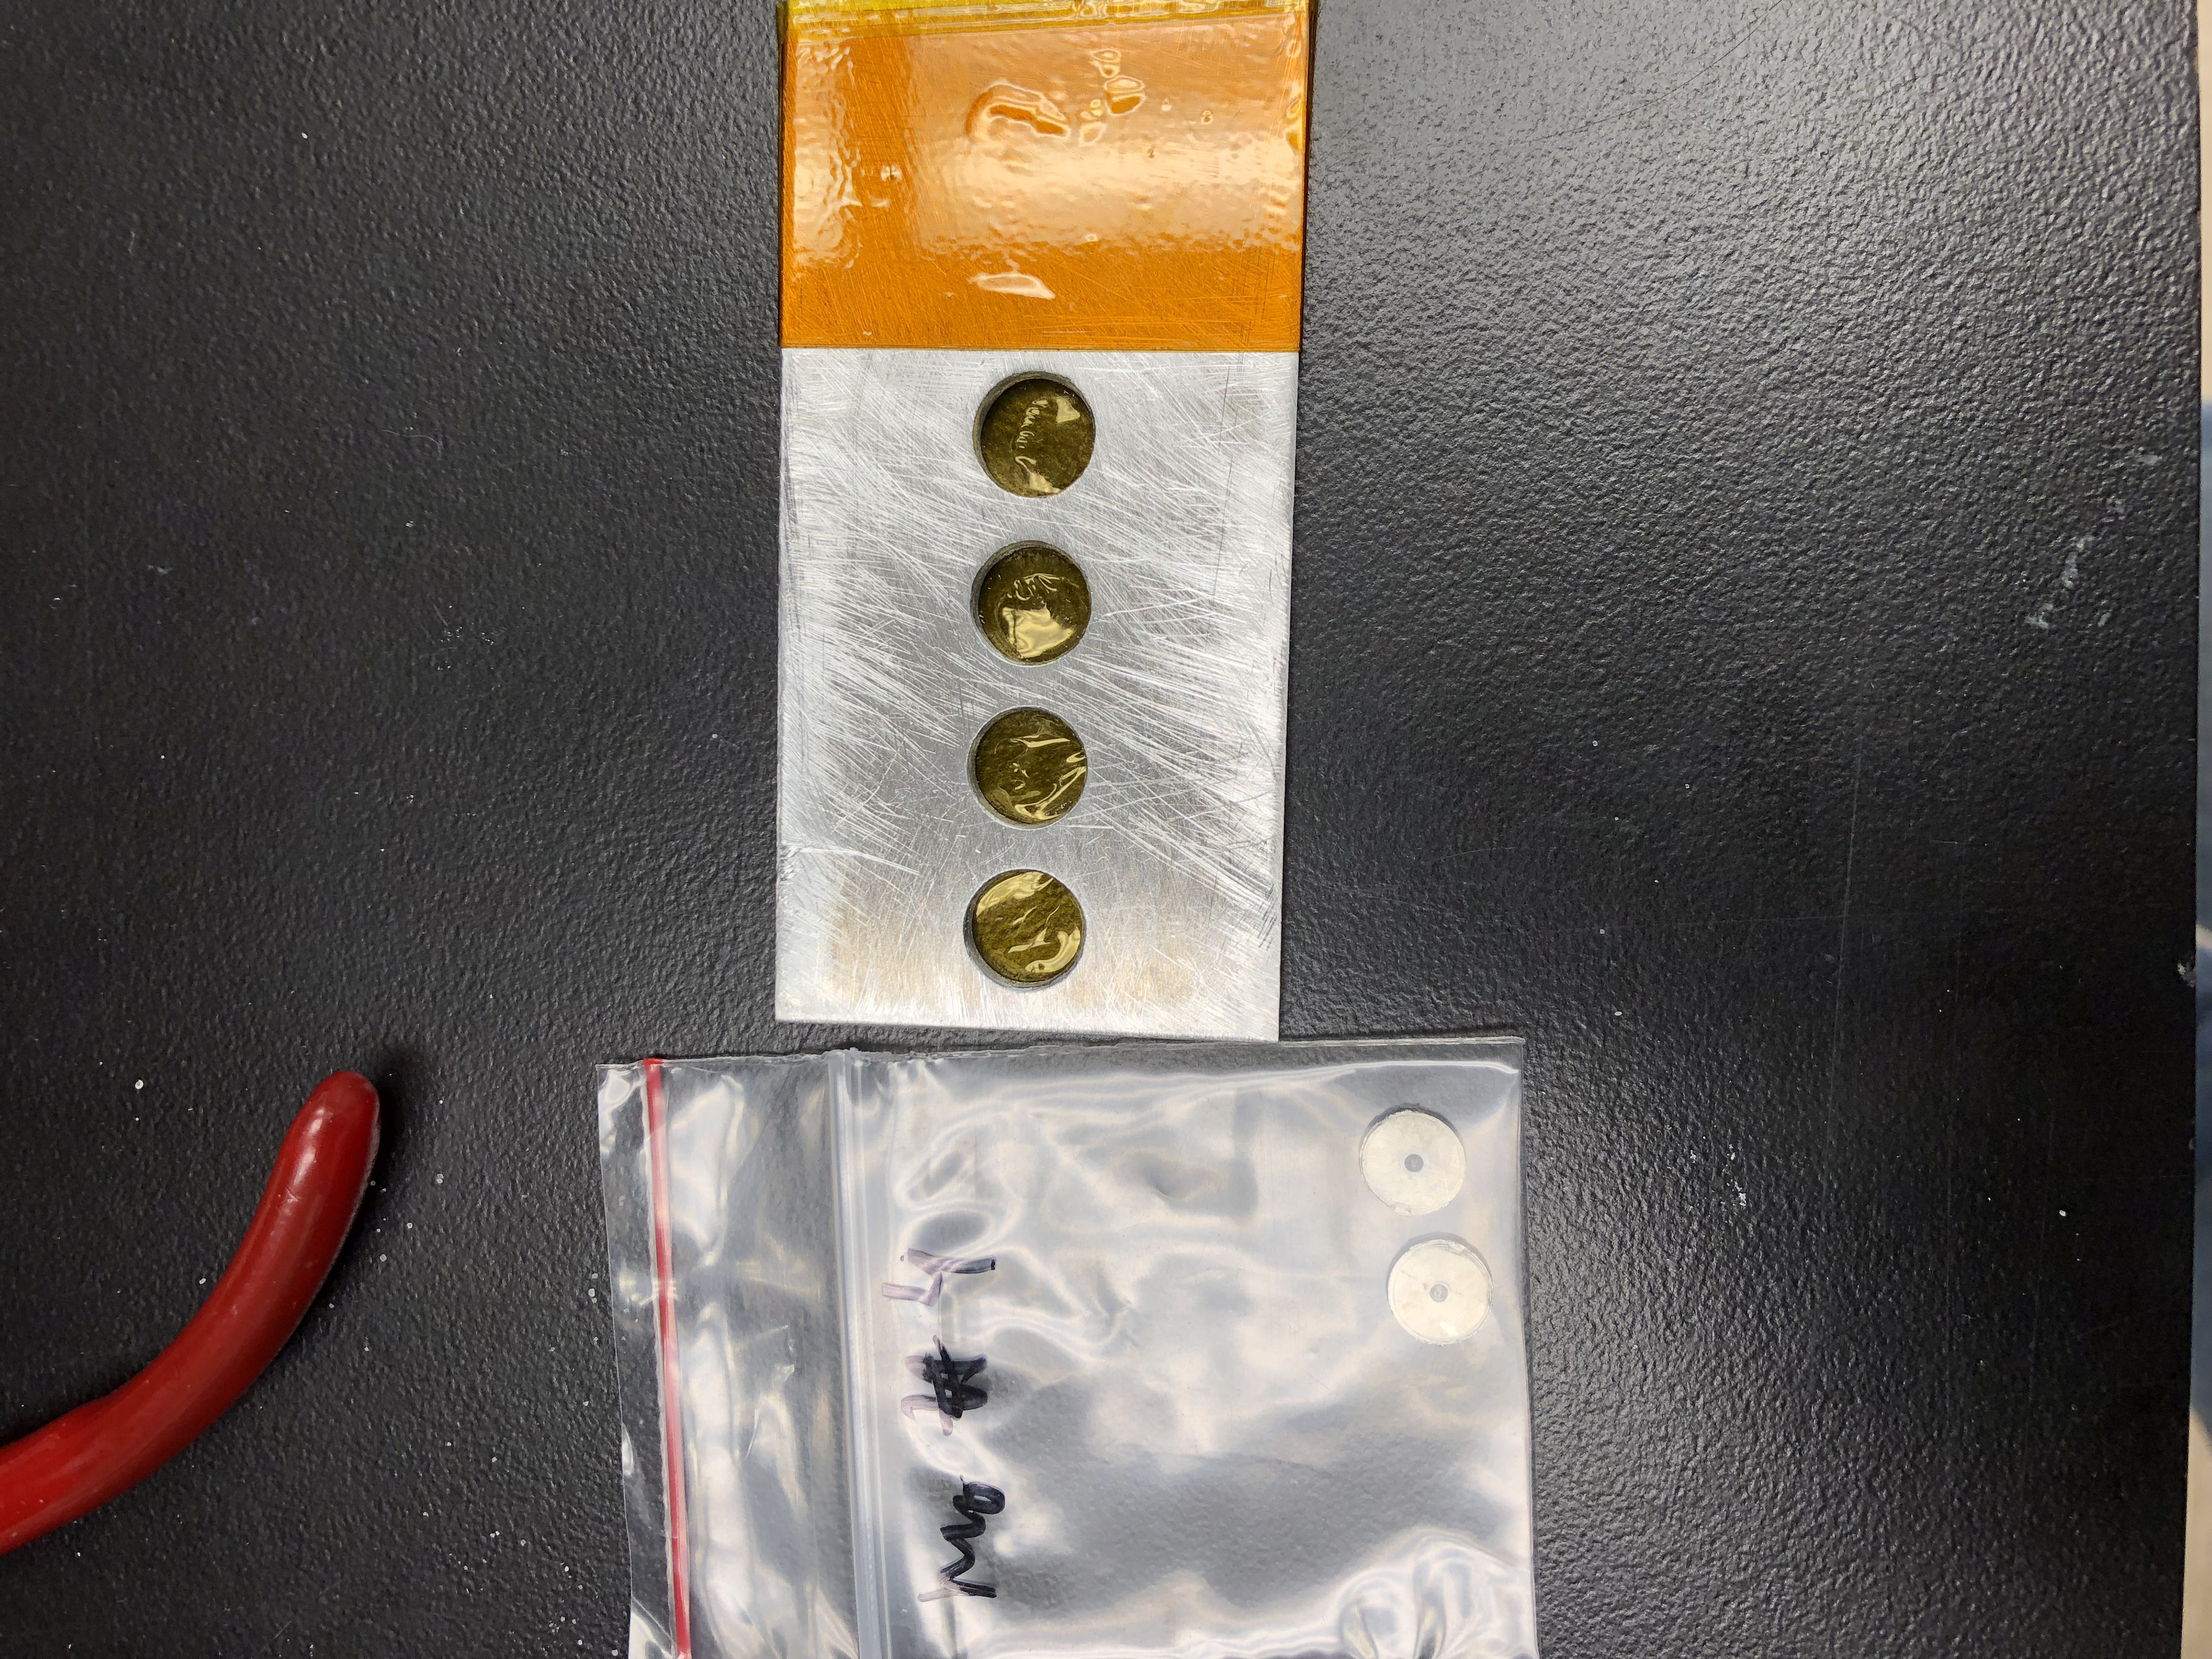
\includegraphics[width=0.75\columnwidth,angle=270]{./figures/IMG_8840.JPG}
 
\includegraphics[width=0.75\columnwidth]{./figures/ipf_beamline_schematic.png}
 % IMG_8840.JPG: 4032x3024 pixel, 72dpi, 142.24x106.68 cm, bb=0 0 4032 3024
 \caption{the 977858699167c3aeabdb.}
 \label{fig:ipf_beamline_schematic}
\end{figure}



\begin{figure}
 \centering
%                                l   b      r    top
%  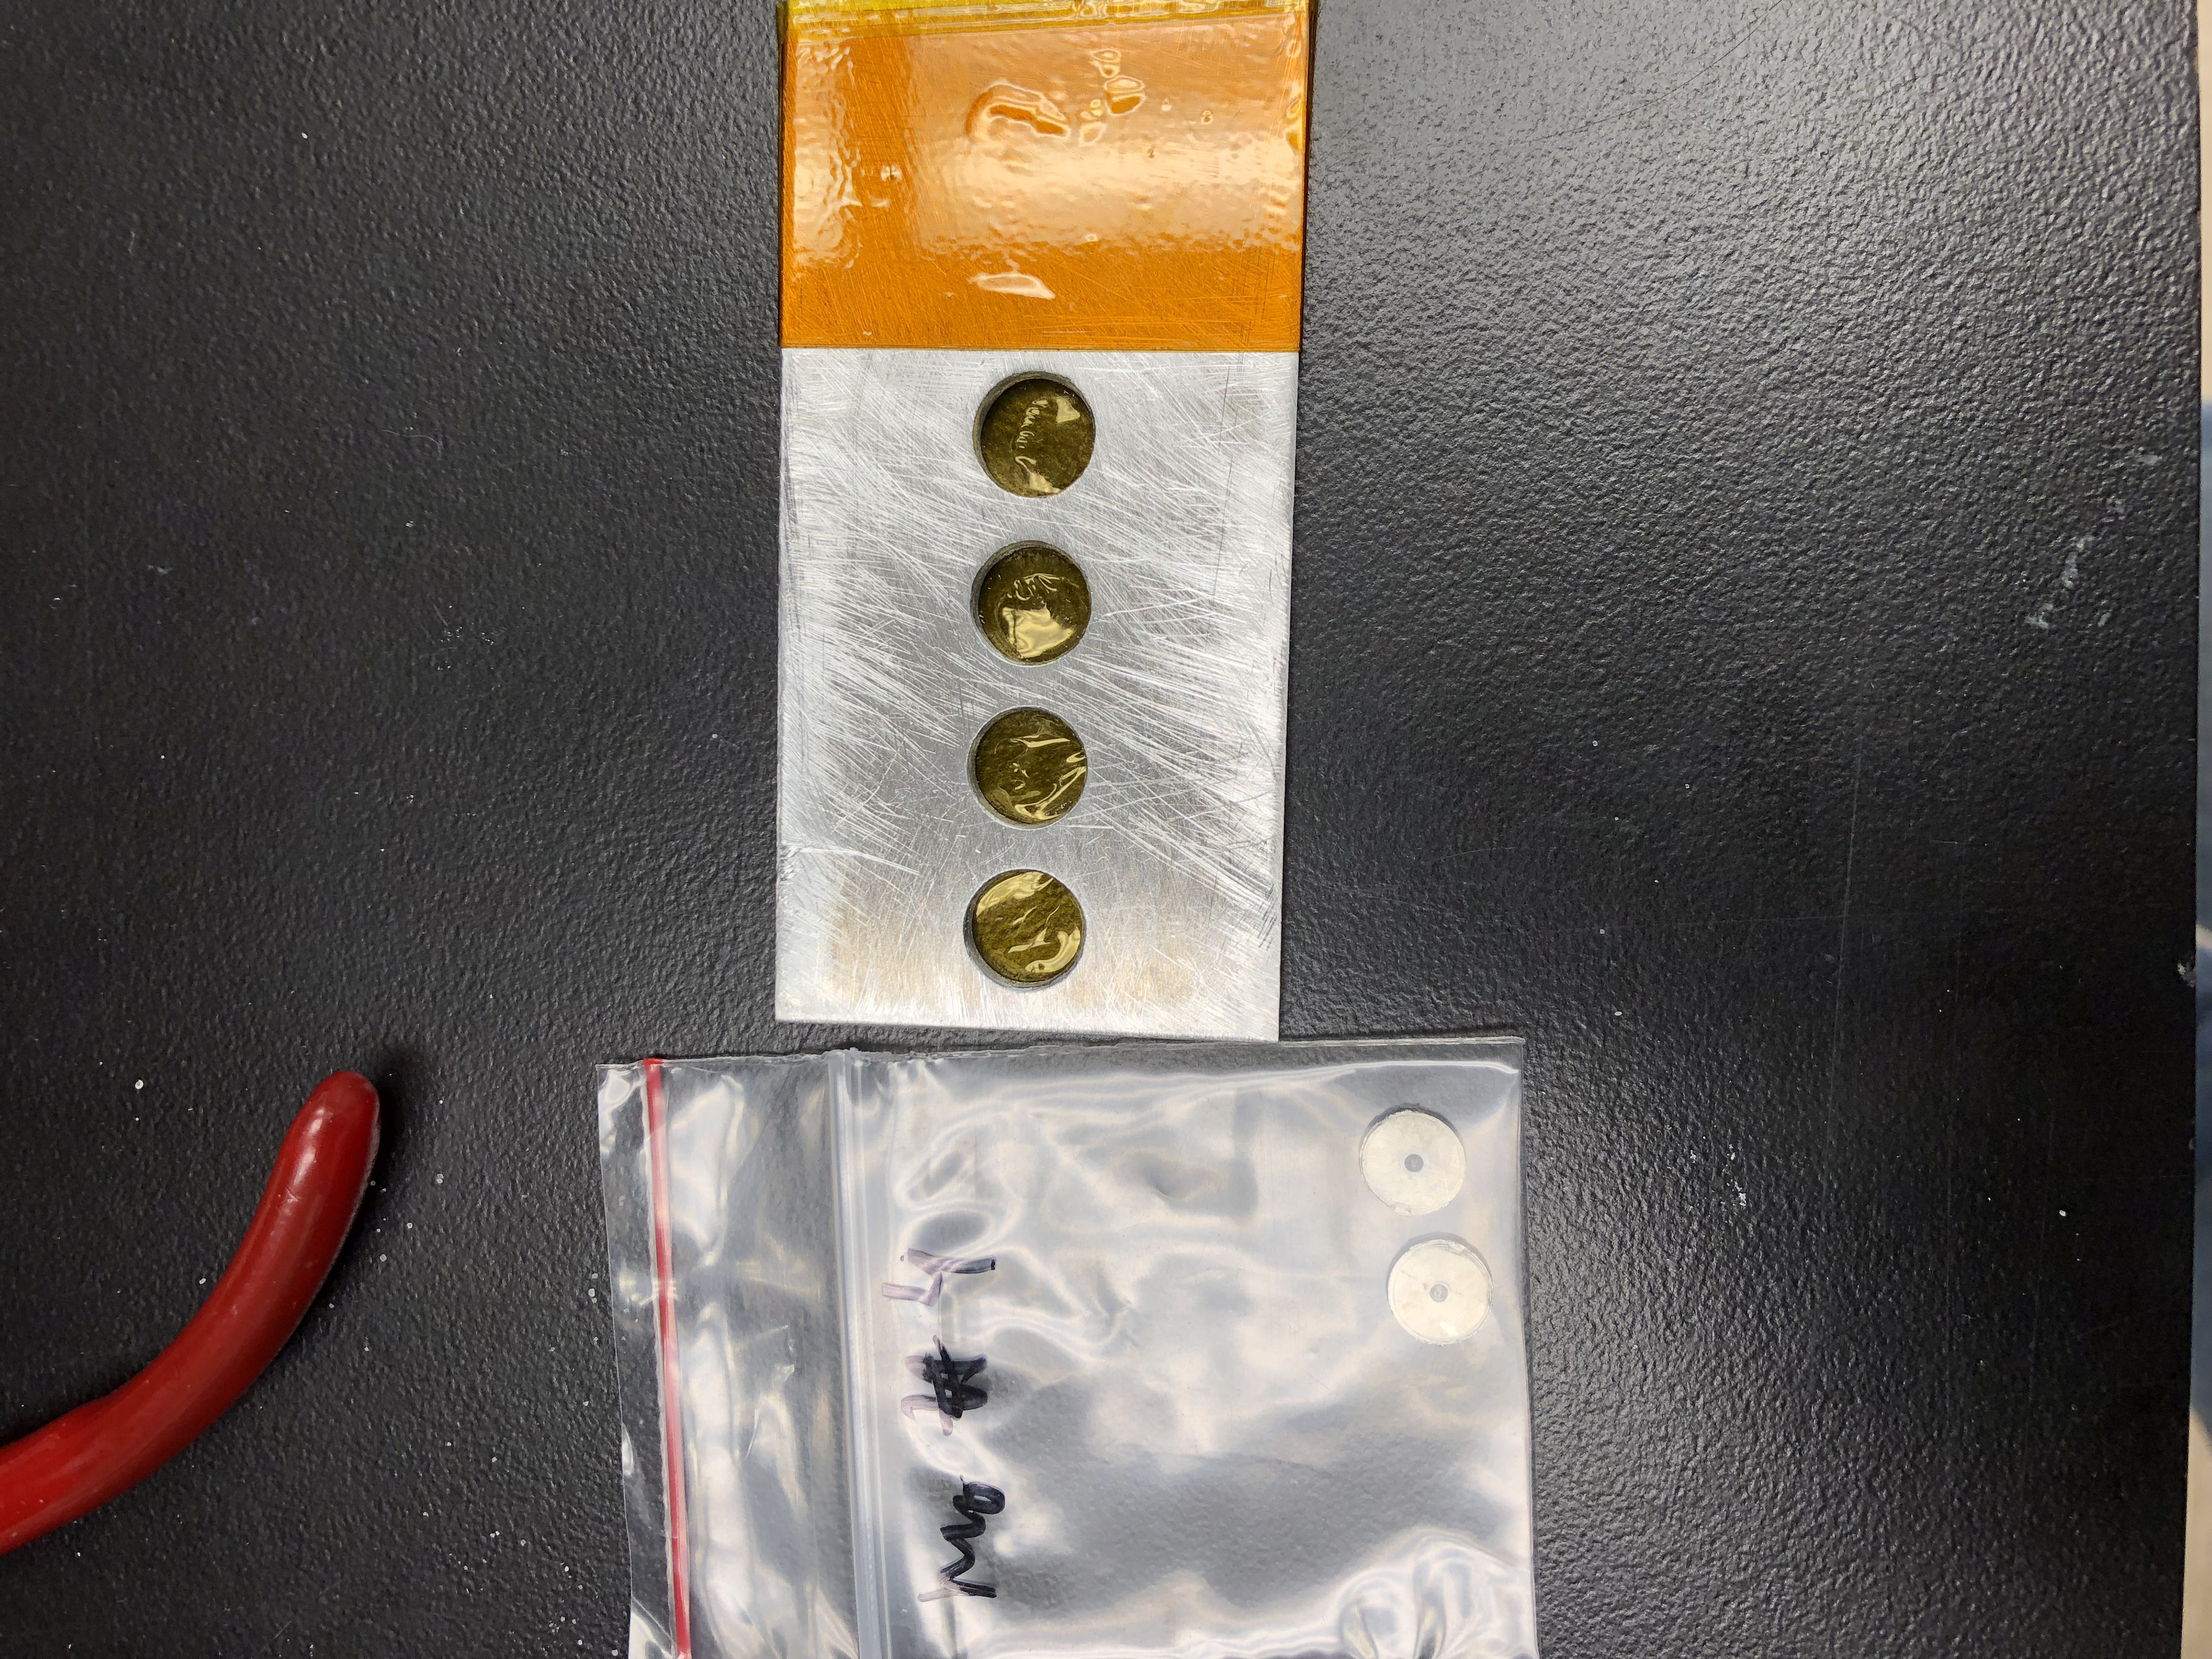
\includegraphics[clip=true,trim=5pt 1000pt 10pt 900pt,width=0.75\columnwidth,angle=90]{./figures/IMG_8840.JPG}
%  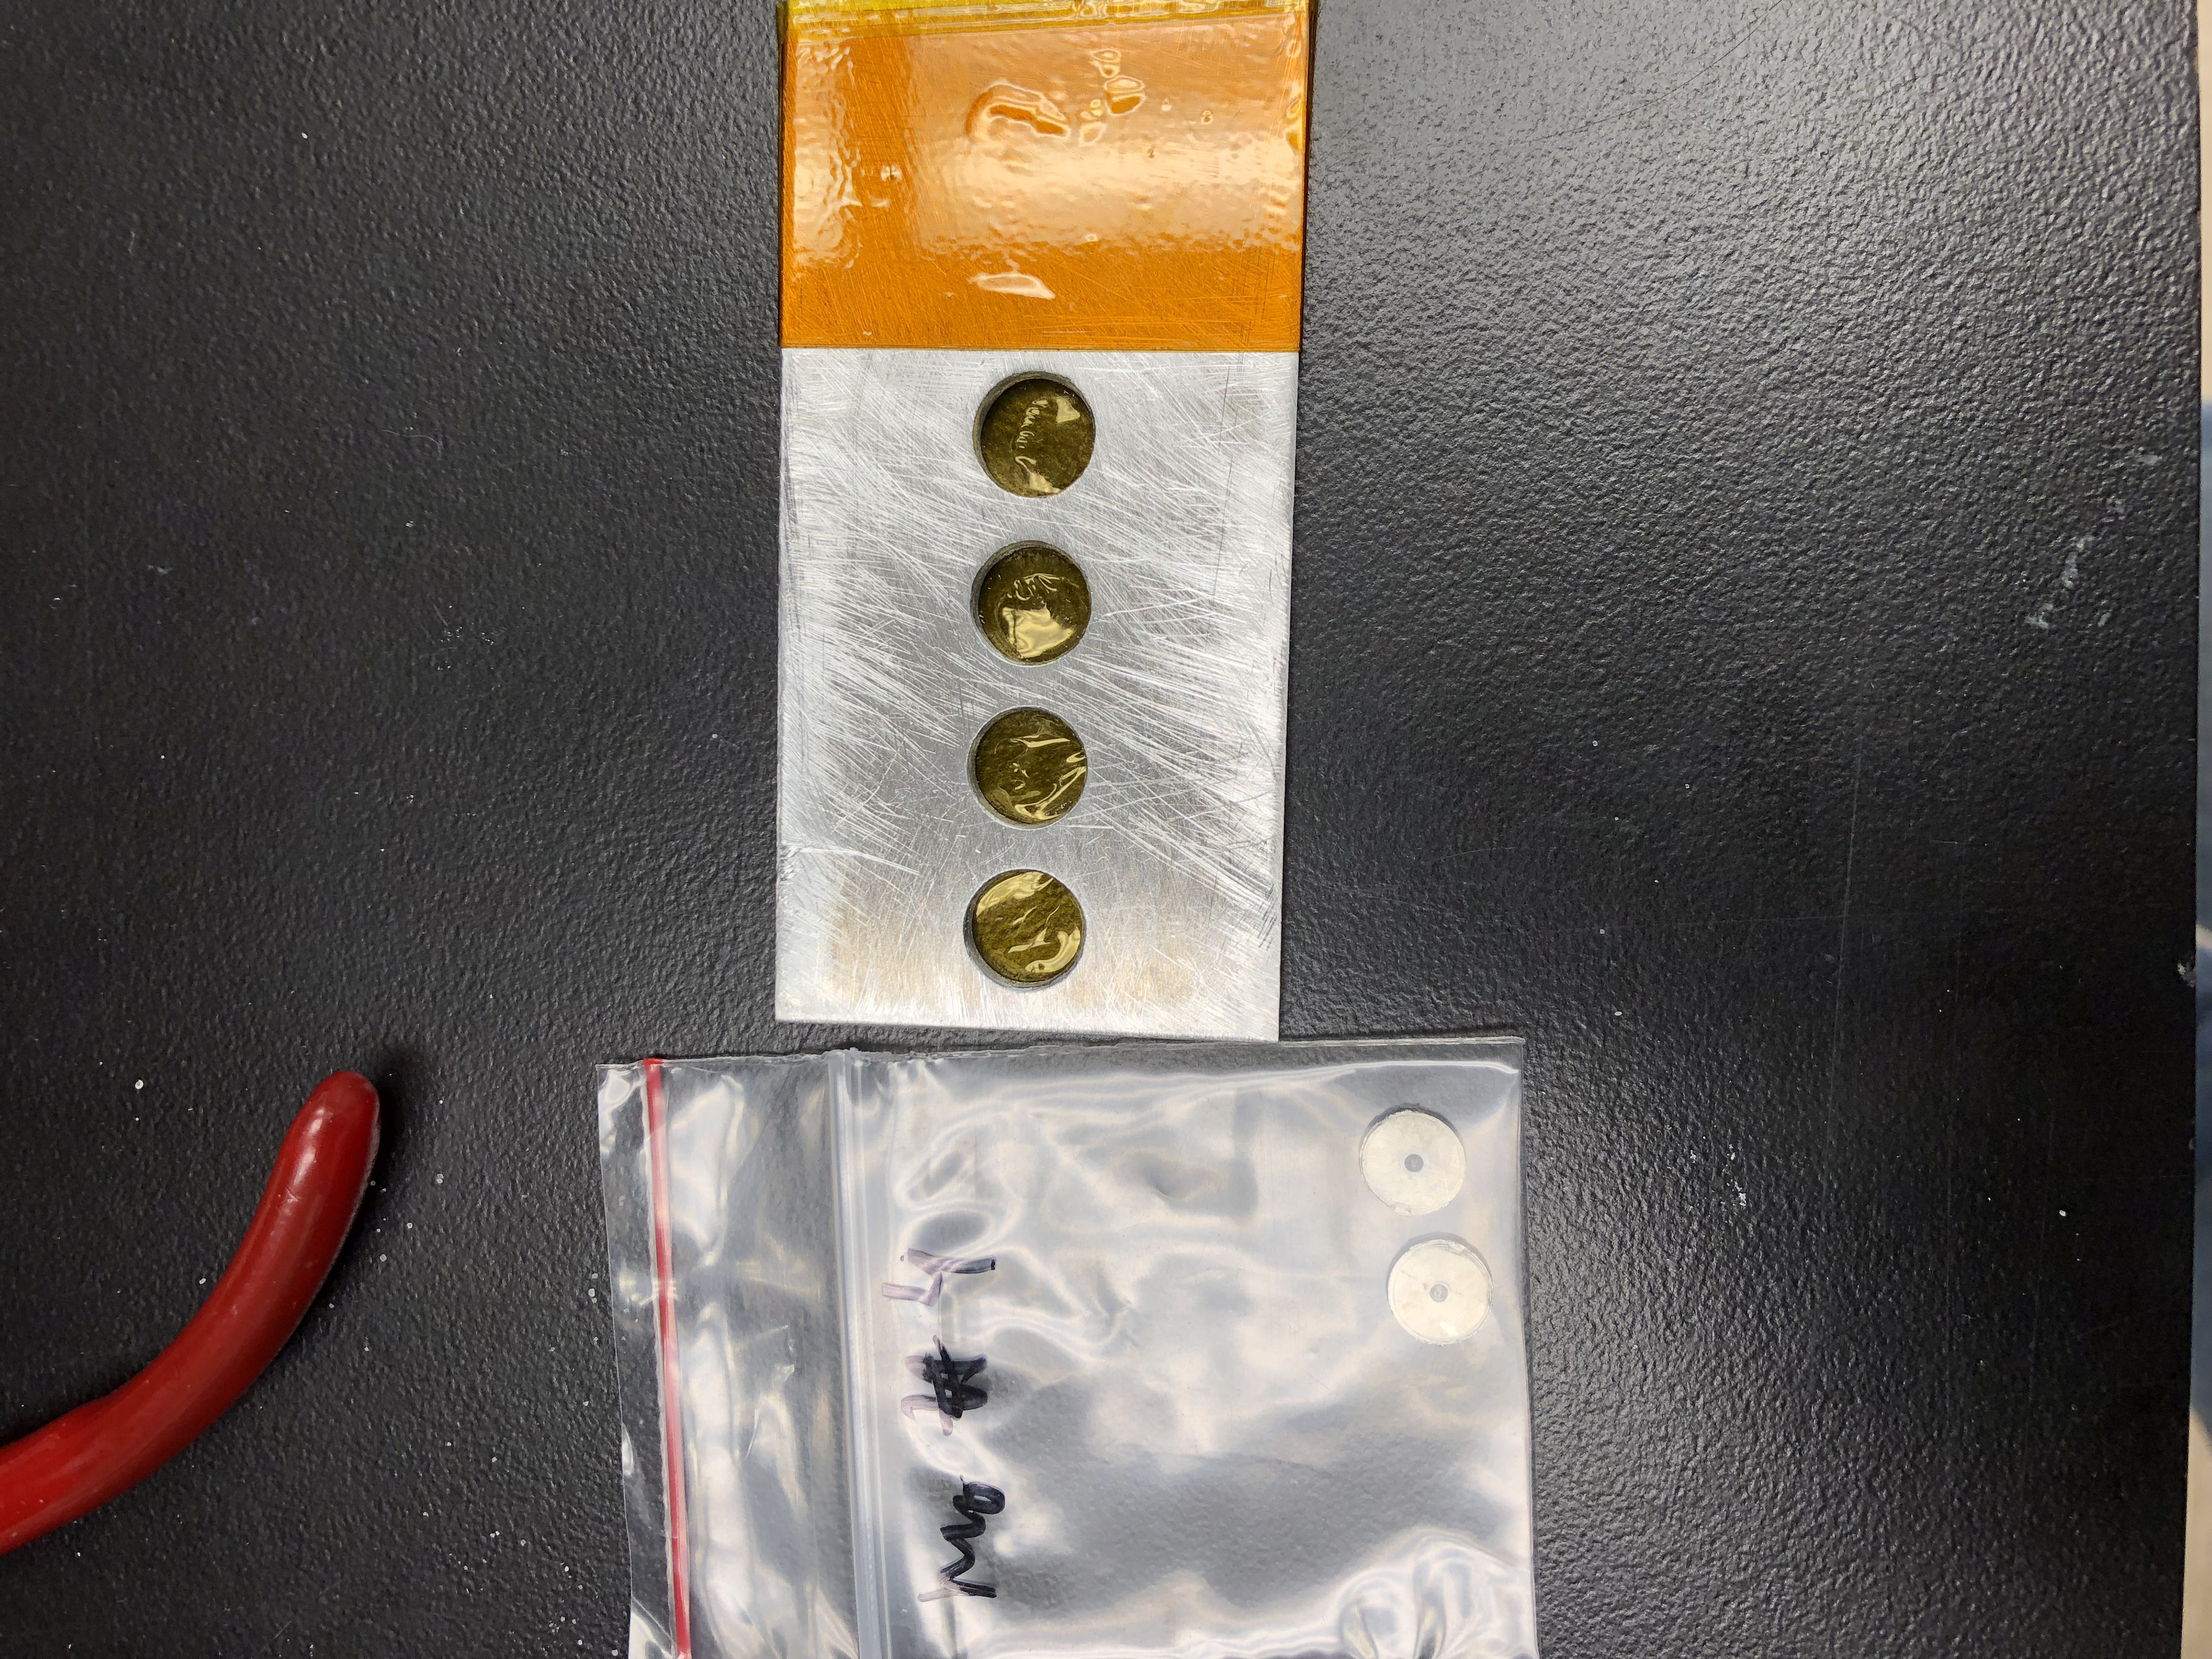
\includegraphics[width=0.75\columnwidth,angle=270]{./figures/IMG_8840.JPG}
 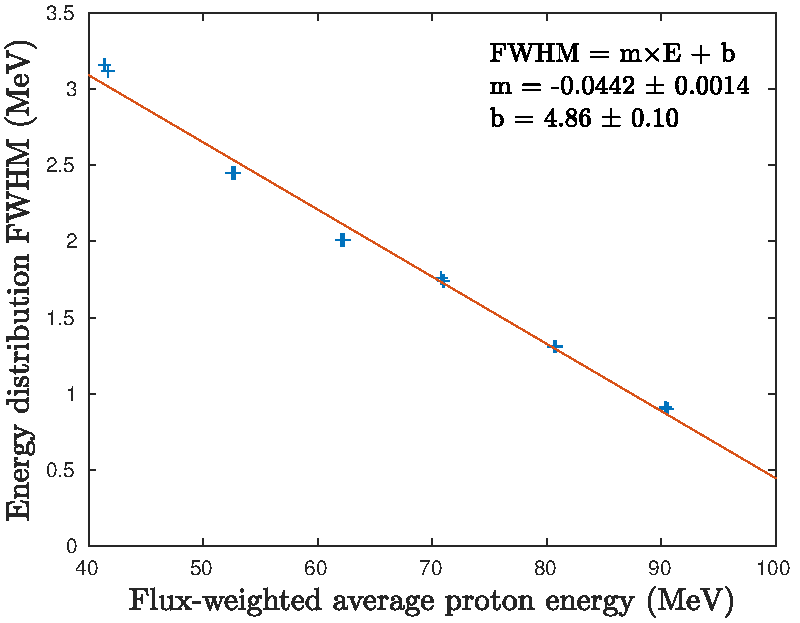
\includegraphics[width=0.5\columnwidth]{./figures/FWHM_plot.pdf}
 % IMG_8840.JPG: 4032x3024 pixel, 72dpi, 142.24x106.68 cm, bb=0 0 4032 3024
 \caption{the FWHM plot.}
 \label{fig:FWHM_plot}
\end{figure}





\begin{figure*}
    \centering    
    \subfloat{
        \centering
%         \includegraphics[width=\textwidth]{./figures/target2.png}
        \subfigimg[width=0.495\textwidth]{}{./figures/22Na.pdf}{80}
%         \caption{Decay curve for the $\beta^-$ decay of \ce{^{116}In}.}
        %         \refstepcounter{subfigure}
%          \label{fig:91mNb}
%    }
%      \subfloat{
%         \centering
%         \includegraphics[width=\columnwidth]{./figures/Capture.PNG}
        \subfigimg[width=0.495\textwidth]{}{./figures/24Na.pdf}{80}
%         \caption{ Decay curve for the $\beta^+$ decay of \ce{^{64}Cu}.}
%         \refstepcounter{subfigure} 
%         \label{fig:92mNb}
   \hspace{-10pt}}%
    \caption{Decay curves used to verify photopeak transition assignment. (a) Decay curve for the isomeric transition of \ce{^{115m}In}, (b) decay curve for the isomeric transition of \ce{^{113m}In}, and (c) decay curve for the $\beta^-$ decay of \ce{^{116}In}.}
%      \phantomcaption{}
     \label{fig:tentative_ipf_na}
\end{figure*}


\begin{figure}
 \centering
%                                l   b      r    top
%  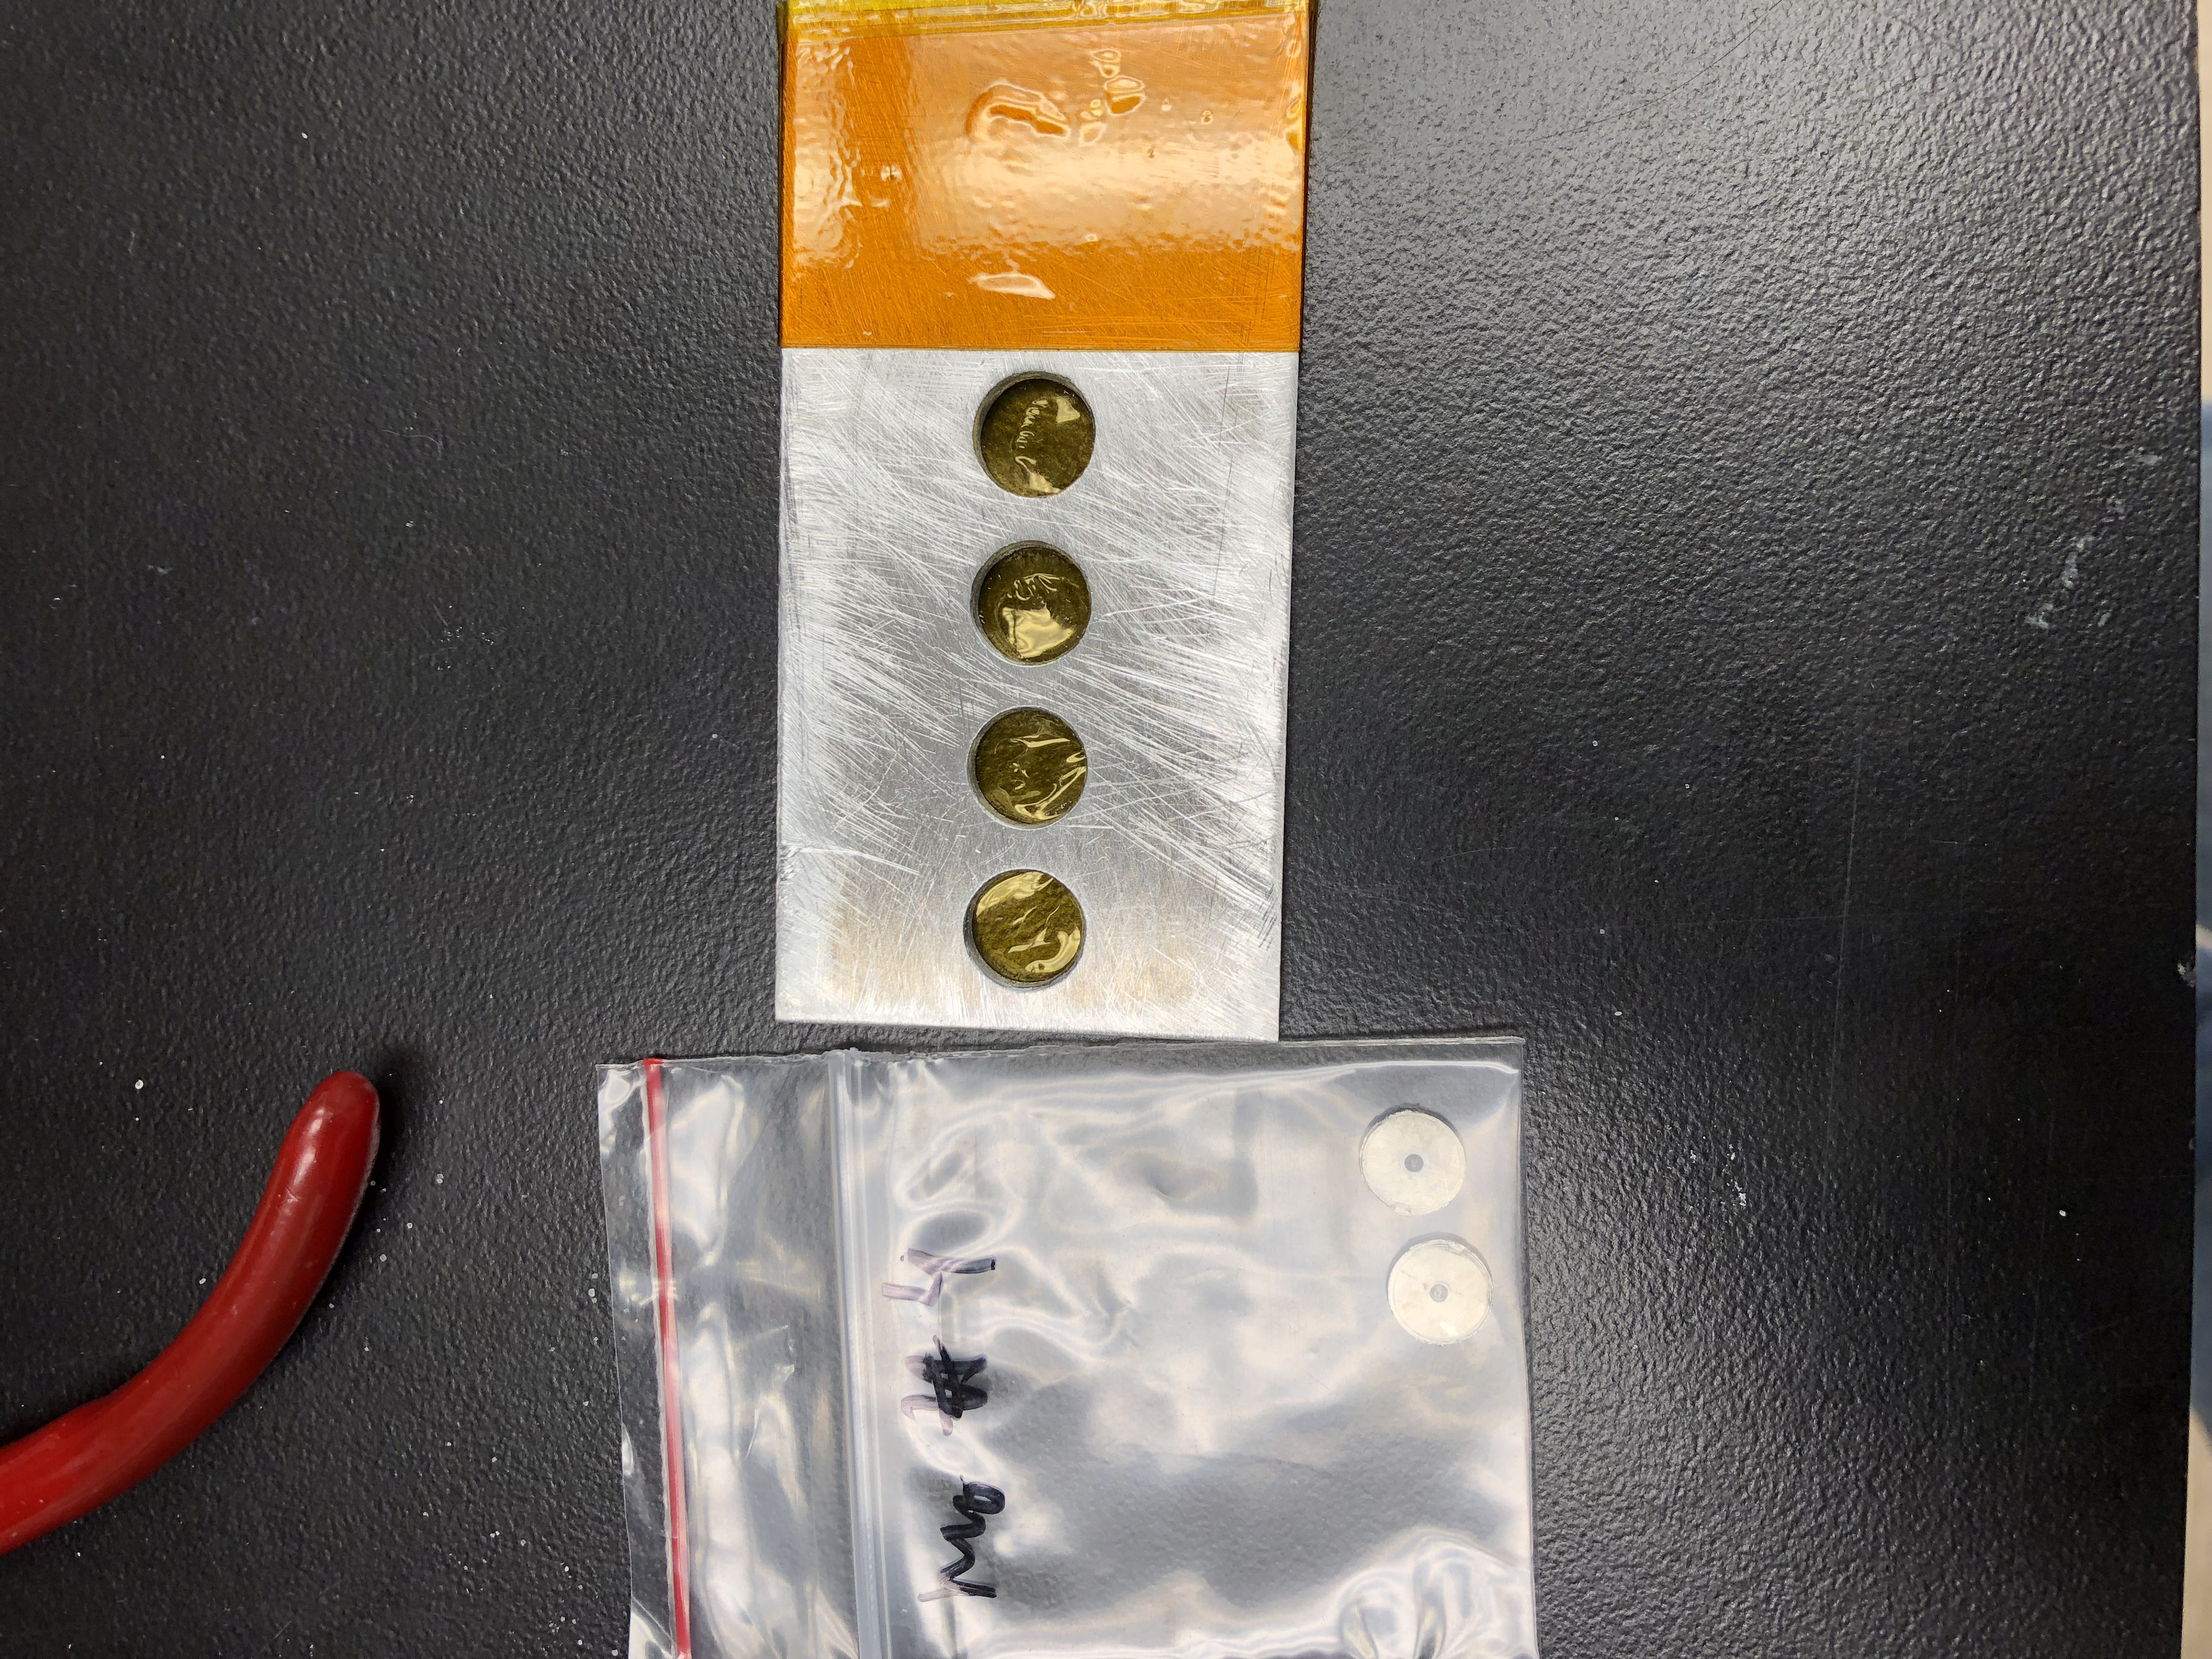
\includegraphics[clip=true,trim=5pt 1000pt 10pt 900pt,width=0.75\columnwidth,angle=90]{./figures/IMG_8840.JPG}
%  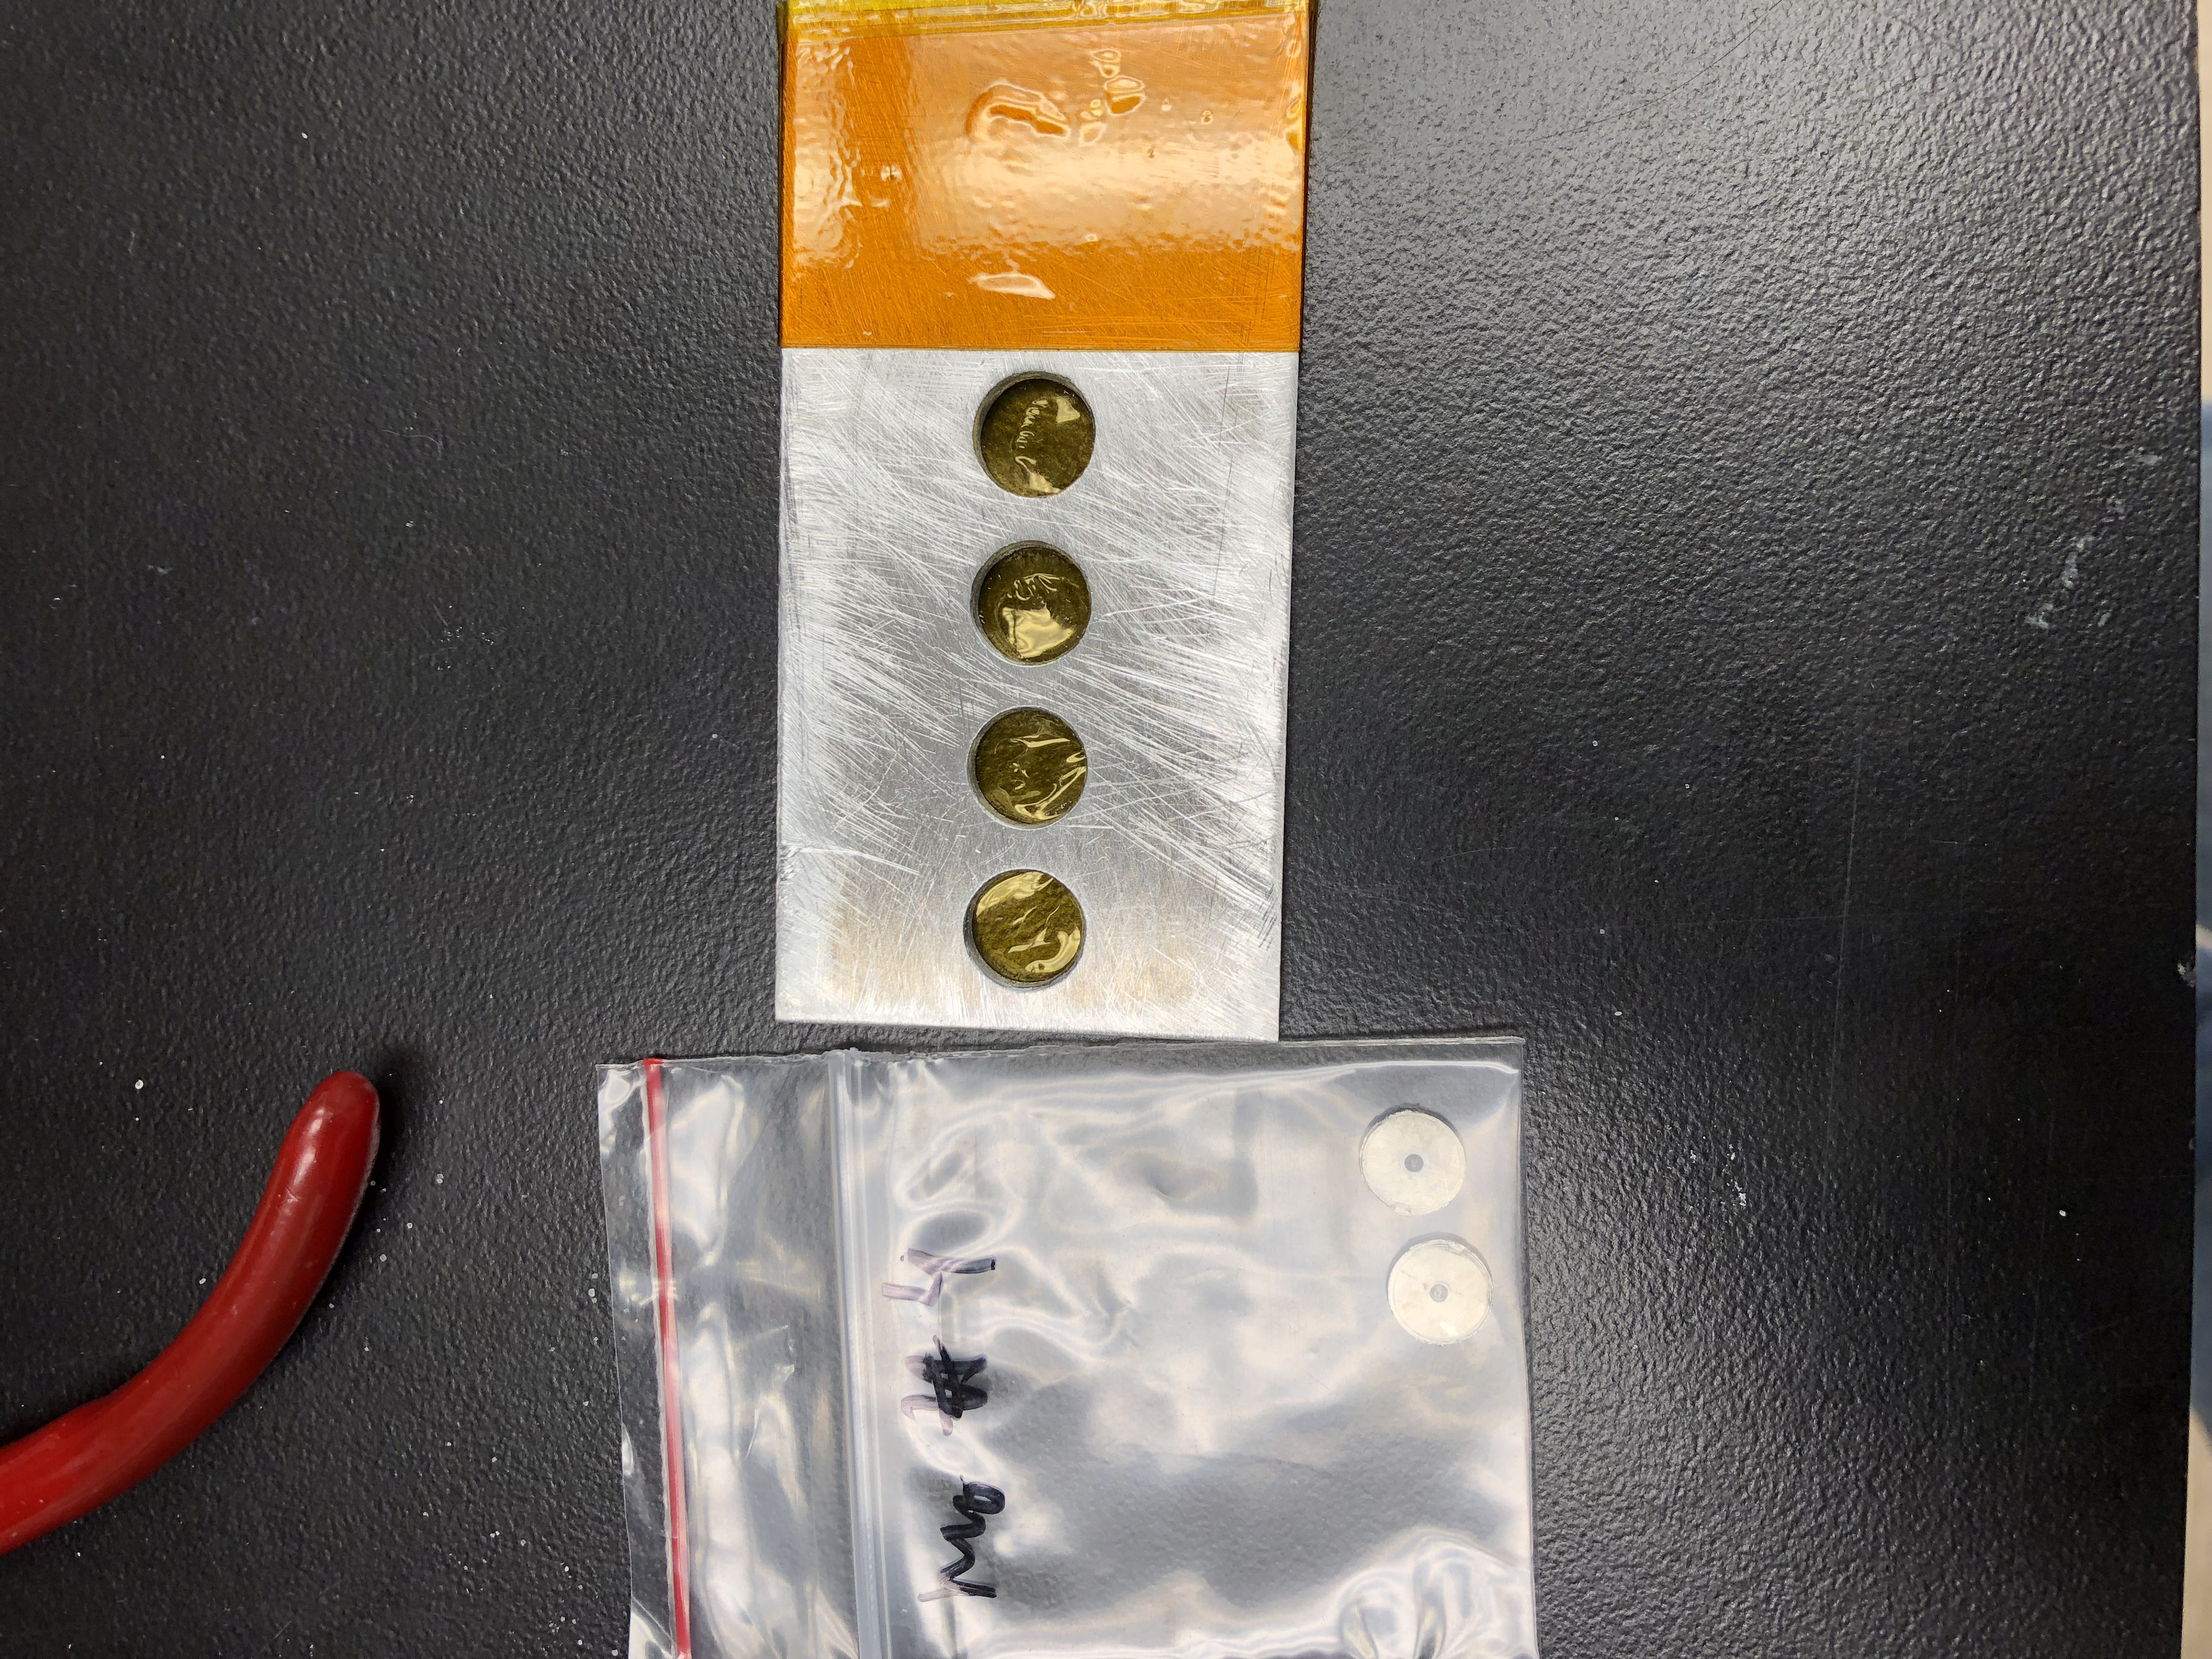
\includegraphics[width=0.75\columnwidth,angle=270]{./figures/IMG_8840.JPG}
 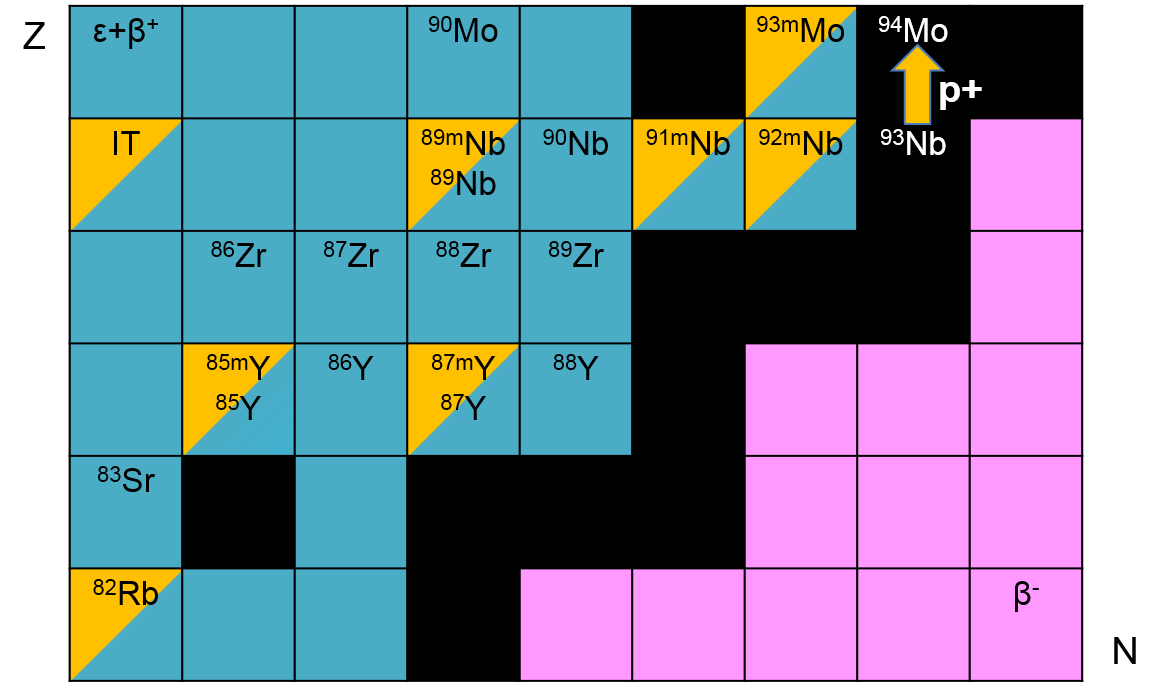
\includegraphics[width=0.75\columnwidth]{./figures/ipf_nb_product_table.png}
 % IMG_8840.JPG: 4032x3024 pixel, 72dpi, 142.24x106.68 cm, bb=0 0 4032 3024
 \caption{the FWHM plot.}
 \label{fig:ipf_nb_product_table}
\end{figure}


\begin{figure}
 \centering
%                                l   b      r    top
%  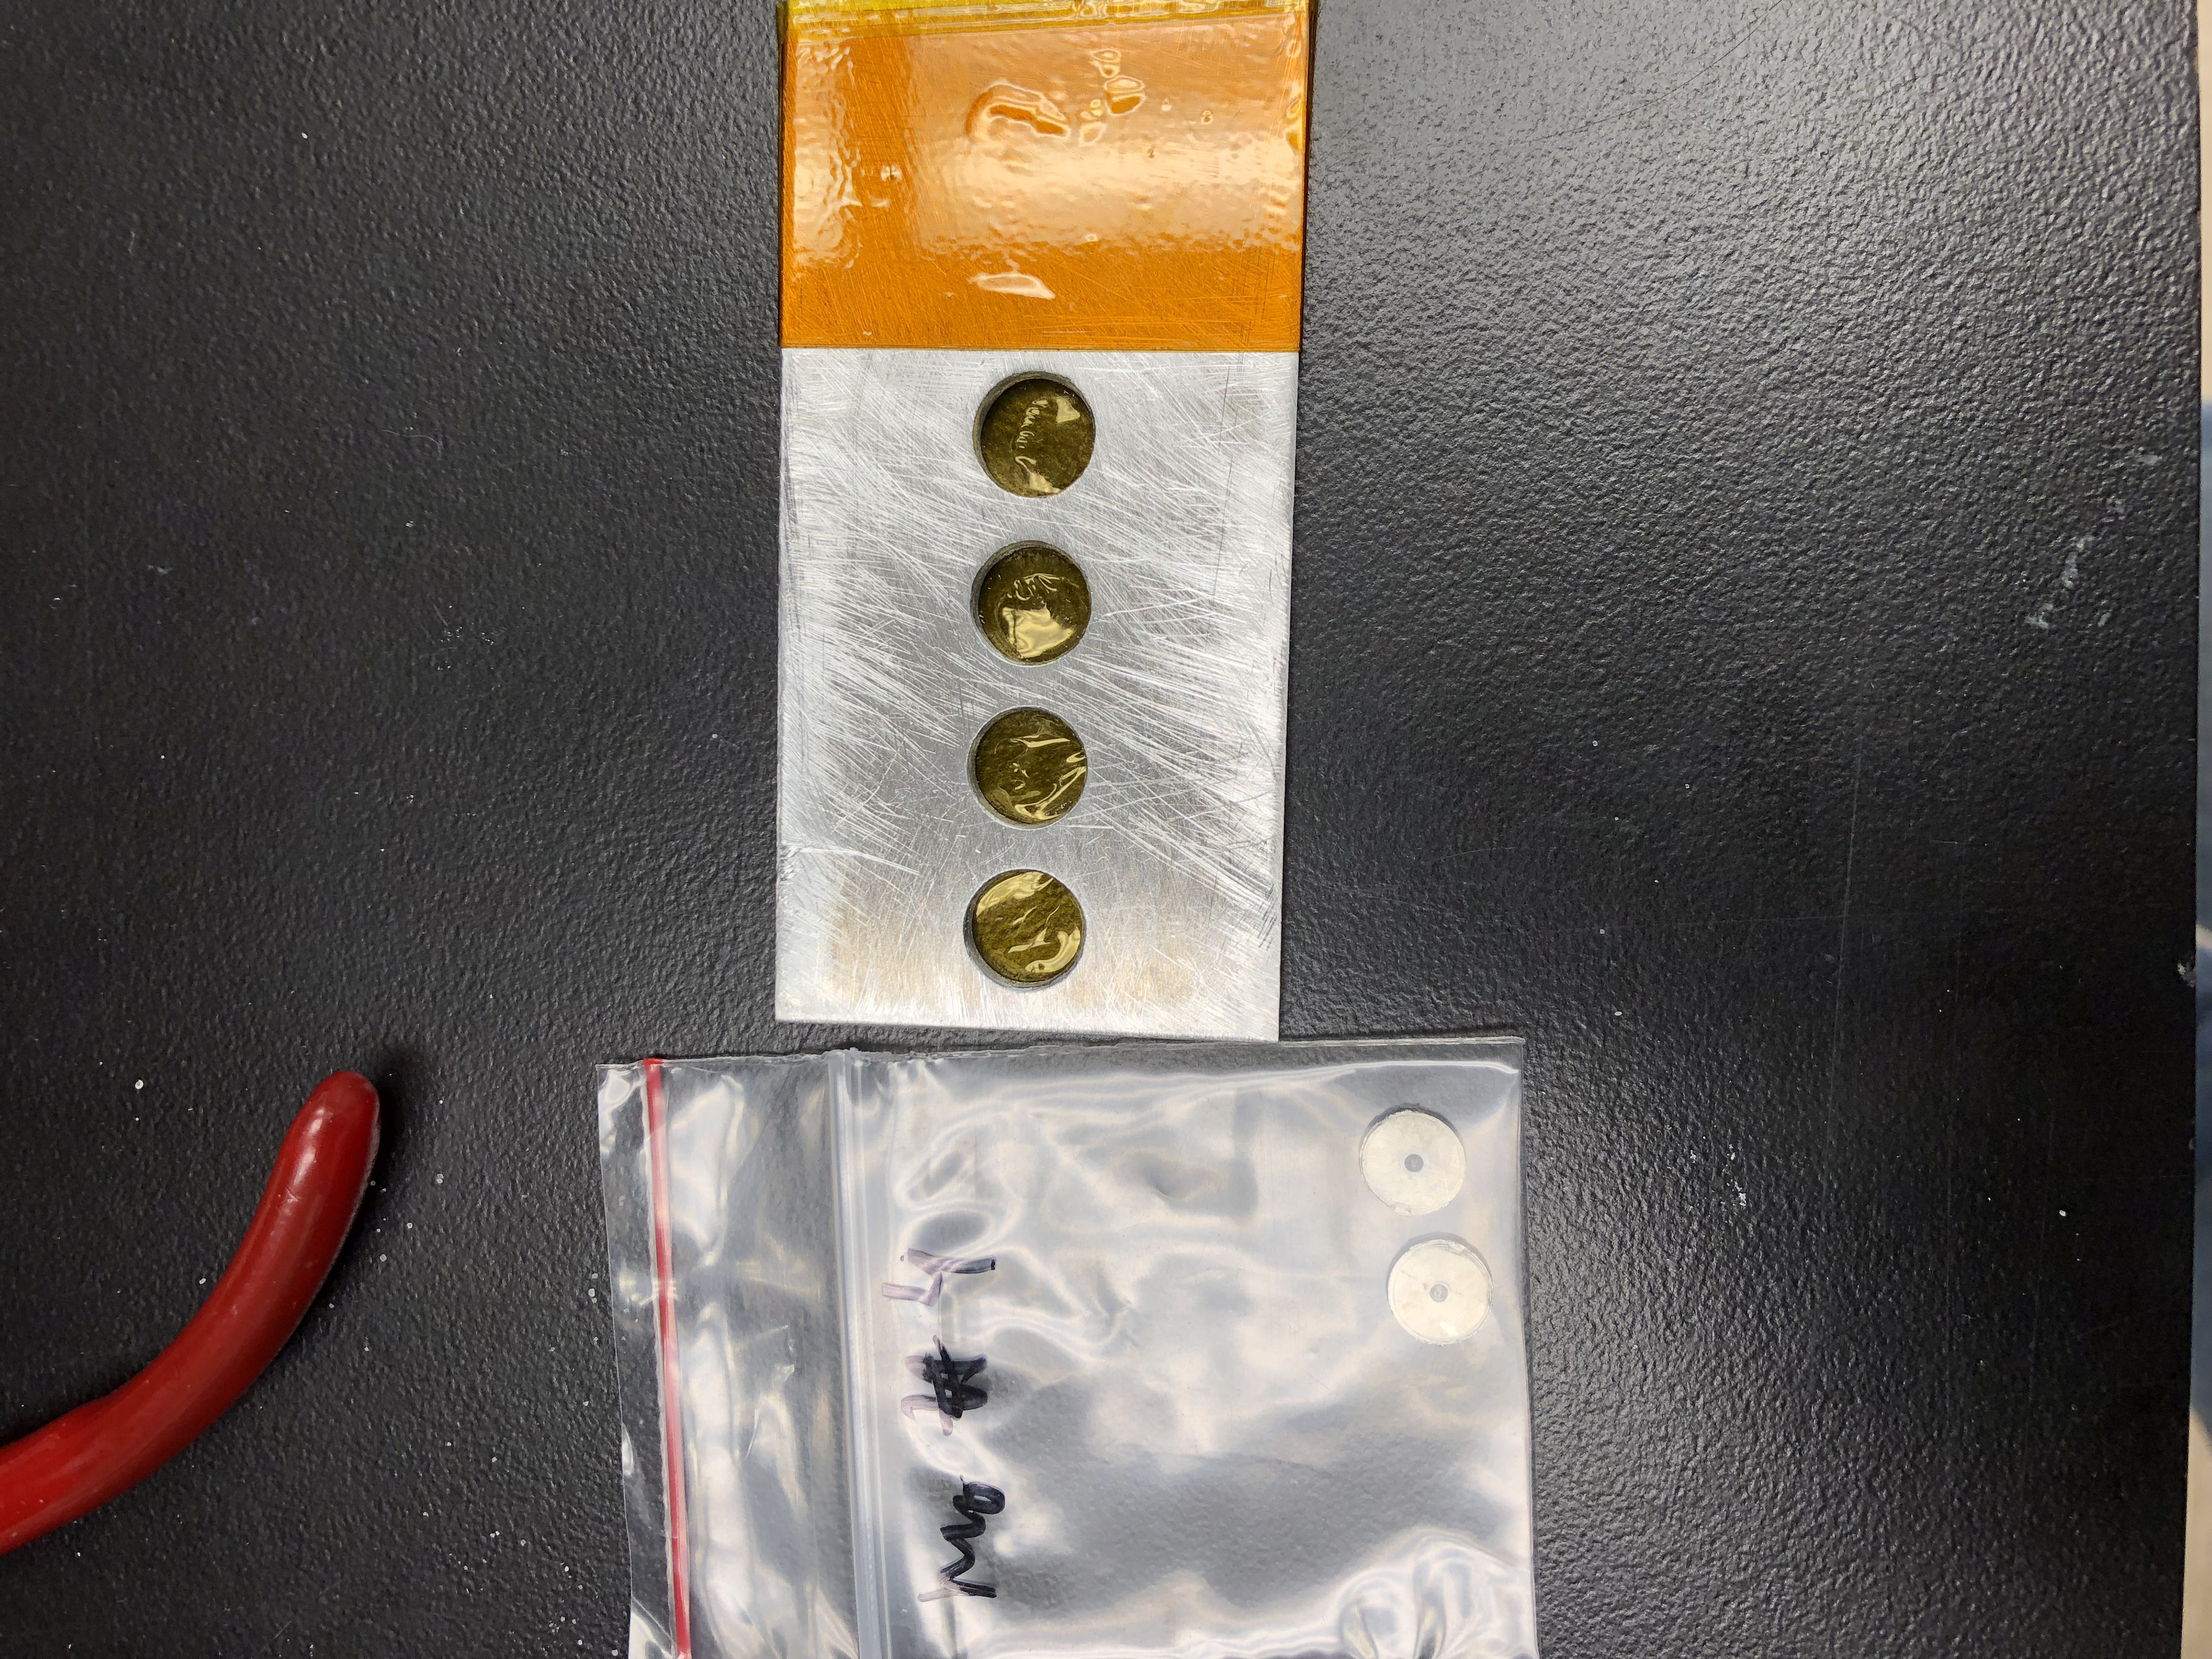
\includegraphics[clip=true,trim=5pt 1000pt 10pt 900pt,width=0.75\columnwidth,angle=90]{./figures/IMG_8840.JPG}
%  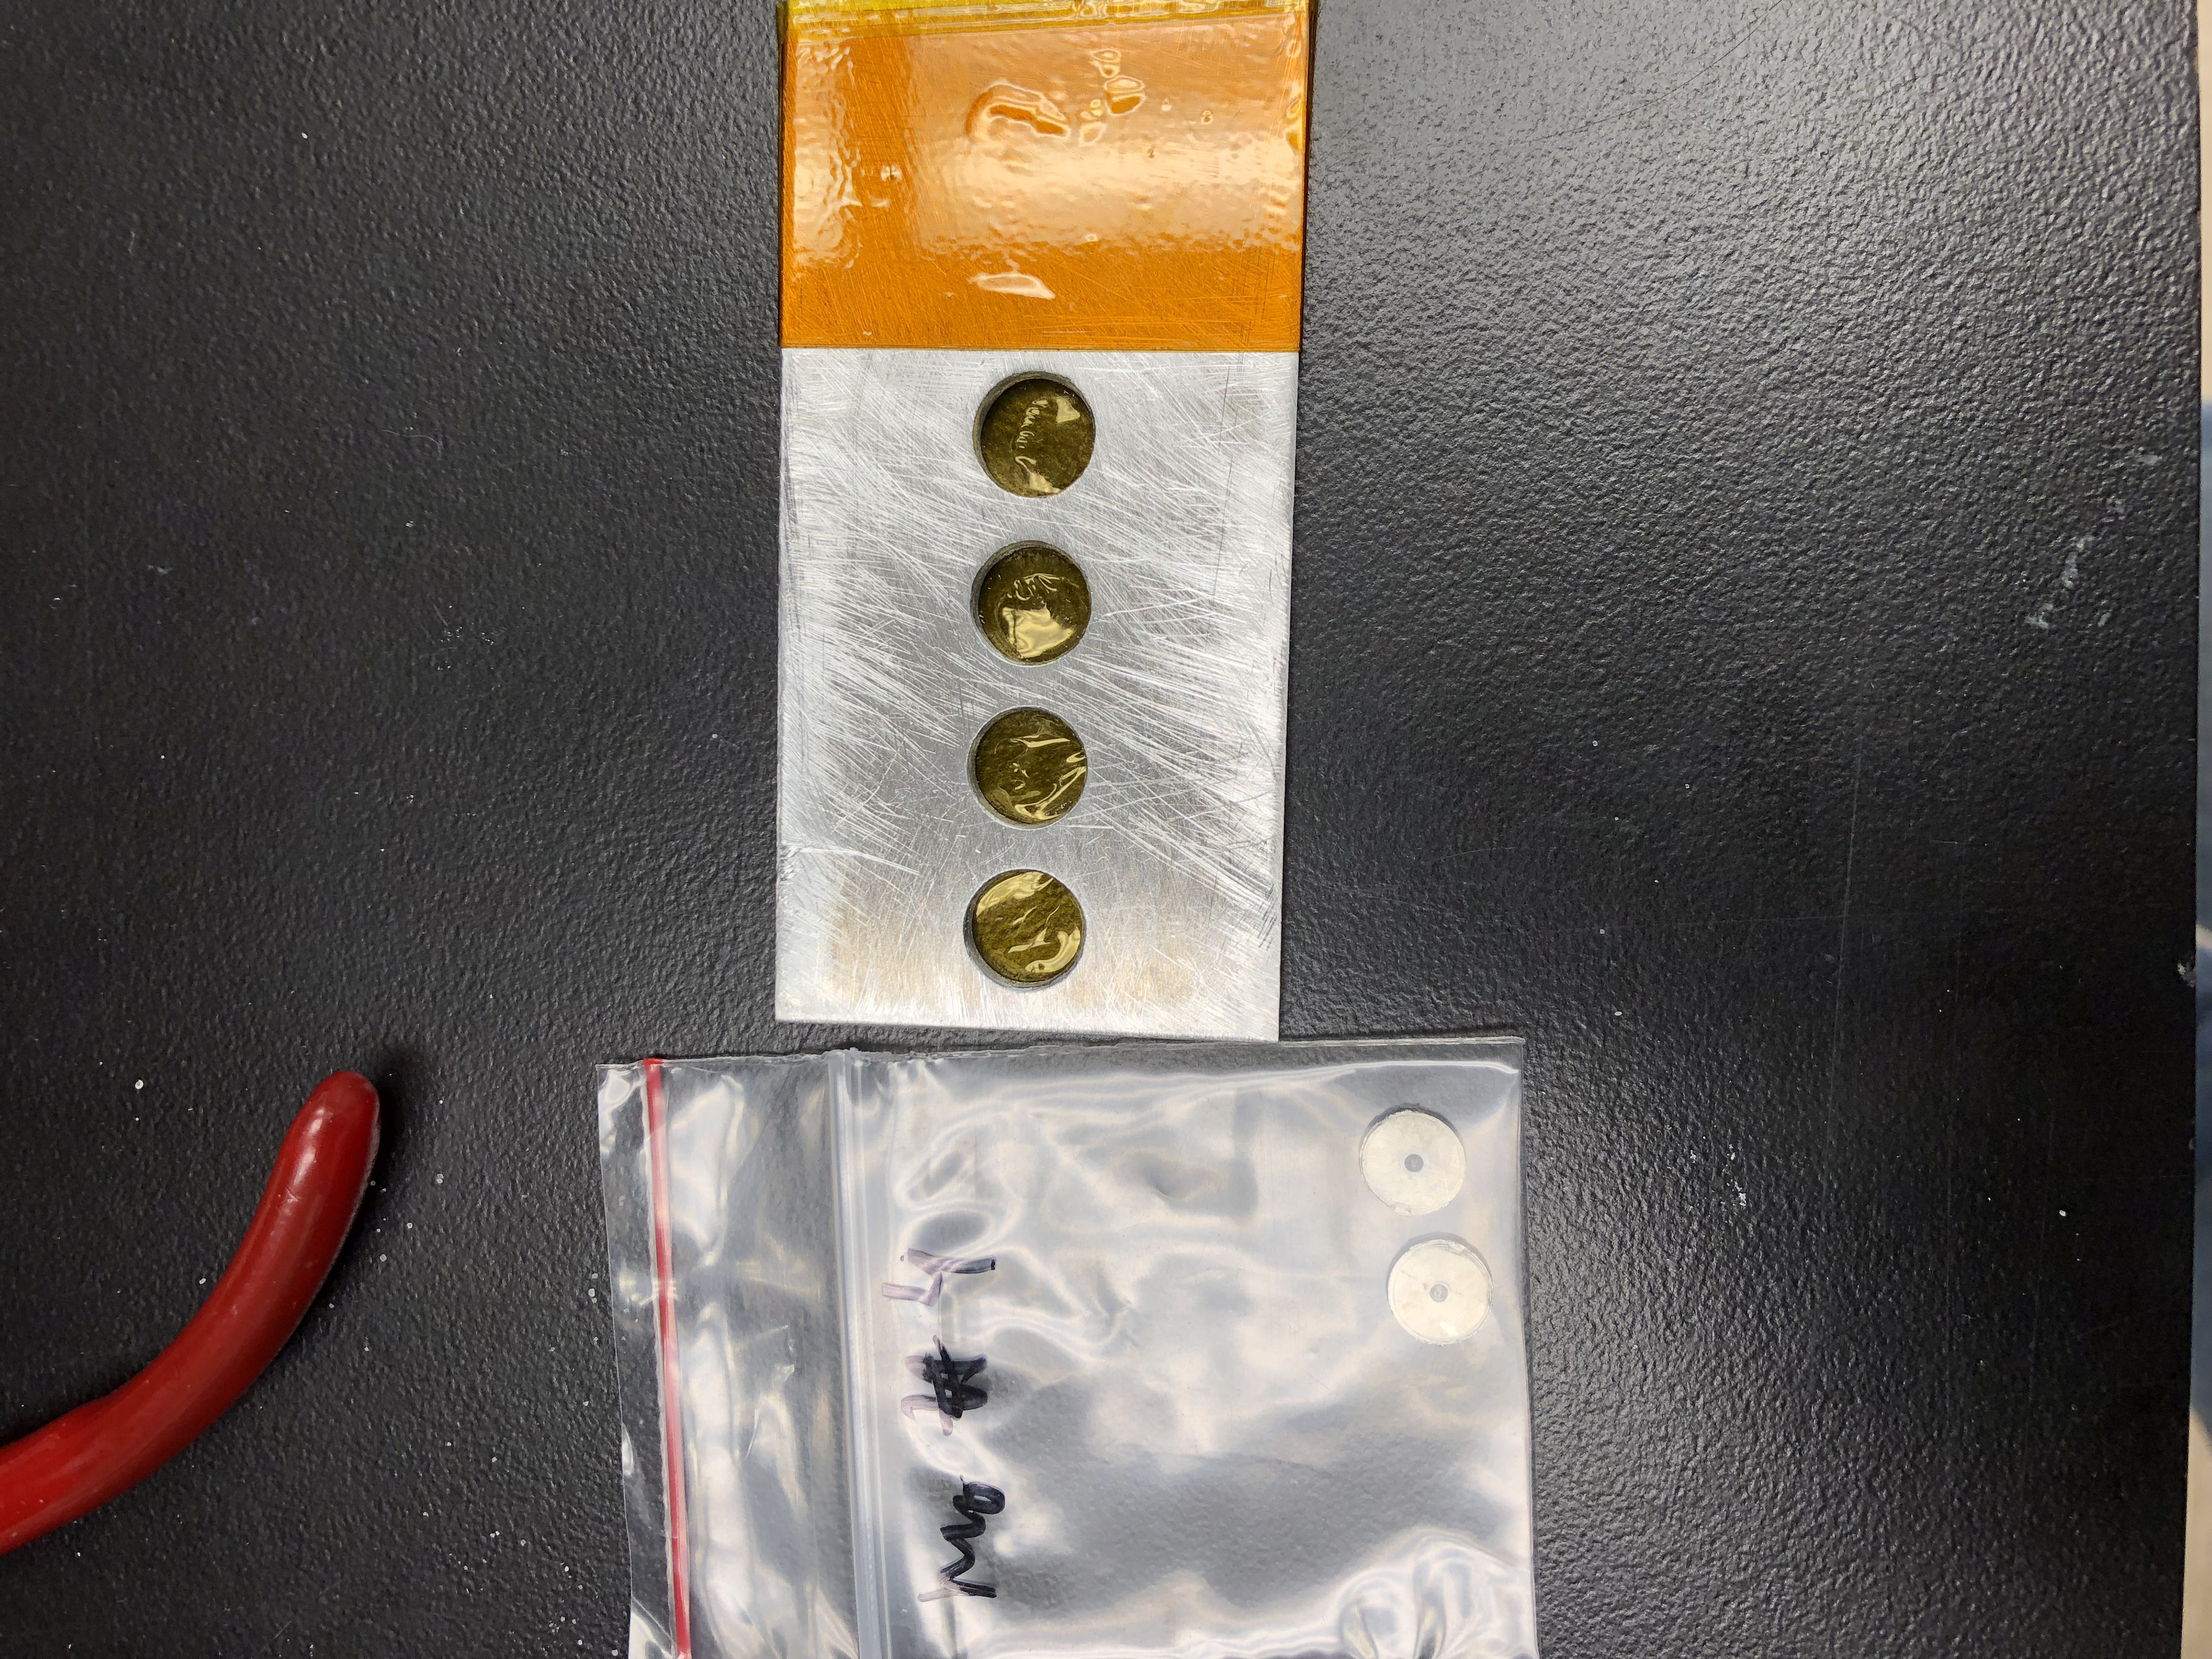
\includegraphics[width=0.75\columnwidth,angle=270]{./figures/IMG_8840.JPG}
 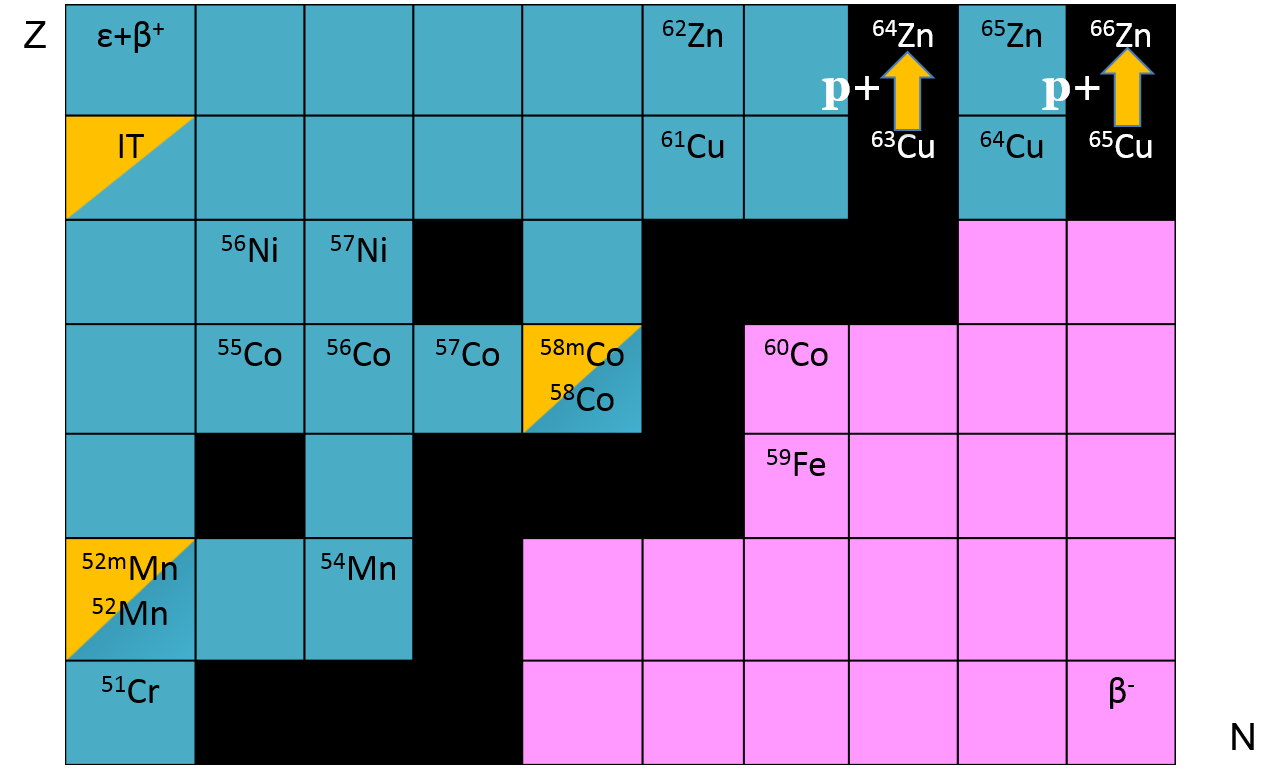
\includegraphics[width=0.75\columnwidth]{./figures/ipf_cu_product_table.png}
 % IMG_8840.JPG: 4032x3024 pixel, 72dpi, 142.24x106.68 cm, bb=0 0 4032 3024
 \caption{the FWHM plot.}
 \label{fig:ipf_cu_product_table}
\end{figure}






% While these TENDL cross sections simply provide approximate \ce{^{nat}Si}(p,x)\ce{^{22,24}Na} yields,  t
There are several important  conclusions to be drawn from this simple estimate using the TENDL   \ce{^{nat}Si}(p,x)\ce{^{22,24}Na} yields.
The observation of the \ce{^{22,24}Na} activities in Cu and Nb foils  represents an indirect measurement of the \ce{^{nat}Si}(p,x)\ce{^{22,24}Na} cross sections, but  will not be reported due to 
% the number of assumptions involved in such a calculation.
uncertainties in the areal density of the Si in the adhesive.
% The EoB \ce{^{22,24}Na} activities have been measured directly, but to convert these into absolute cross sections, accurate knowledge of the precise silicone composition and areal density are required.
% These have been taken as
However, if we assume a 10\% Si stoichiometric basis and an areal density of 4.79\,mg/cm$^2$ (based on bulk density),
% respectively, for the purposes of transport calculations, but this level of confidence is insufficient for the reporting of a cross section.
% In principle, it would be possible  to 
we can subtract out the measured \ce{^{22,24}Na} activity at each Nb and Cu foil position (correcting for the minor difference in proton energy between adjacent foils) from the apparent \ce{^{22,24}Na}  activities observed in each Al foil packet, in order to obtain the \enquote{true} or uncontaminated fluence via the Al monitor reactions, shown  
% The results of this  may be seen 
in \autoref{fig:na_subtraction}.
Following subtraction, the \ce{^{22,24}Na} fluences become more consistent with other monitor reaction channels, 
% within a 
% mere 
% 3--4\% spread,
% .
% While this would circumvent the assumptions needed for reporting \ce{^{nat}Si}(p,x)\ce{^{22,24}Na} cross sections, subtraction of  inaccurately quantified \ce{^{22,24}Na} activity in each Nb and Cu foil would propagate into the final fluence determination at each energy position, shifting the magnitude of all reported cross sections.
% Even following subtraction, 
though  \ce{^{22}Na} fluence remains 3--6\% higher than the weighted mean of the remaining monitor reaction channels.
While the dramatic improvement in monitor reaction consistency builds confidence, in the interest of surety and because they are consistent, only the \ce{^{nat}Cu}(p,x)\ce{^{56}Co}, \ce{^{nat}Cu}(p,x)\ce{^{62}Zn}, and \ce{^{nat}Cu}(p,x)\ce{^{65}Zn} monitor reaction channels will be used for fluence determination for the reported cross sections.
% In both cases, this disparity is caused by the fact that both of these monitor reactions may also form the \ce{^{22}Na} and \ce{^{56}Co} reaction products through contamination by secondary neutron (n,x) channels, increasing the apparent fluence as observed by these monitor reactions.
% Since no method for reliably separating the fraction of \ce{^{22}Na} and \ce{^{56}Co} activities induced through (n,x) exists, the fluences predicted by these monitor channels are not used in the final determination of the proton fluence seen by Nb foils. 
% The fact that this \enquote{extra fluence} diminishes at lower energy is likely attributed to the fact that the \ce{^{nat}Al}(p,x)\ce{^{22}Na} and \ce{^{nat}Cu}(p,x)\ce{^{56}Co} have energetic thresholds of 23.35 and 36.76 MeV, respectively. 
% The fraction of secondary neutrons produced by (p,xn)  which are energetic enough to populate the  \ce{^{22}Na} and \ce{^{56}Co} reaction products at the lower energy positions becomes progressively smaller.
This serves as a pointed example of the importance of selecting monitor reaction products inaccessible through channels aside from the primary reaction (\ce{^{nat}Al}(p,x)\ce{^{22,24}Na}, in this case ), as noted previously.
% However,  the fact that both monitor reactions measure consistently higher fluence than the other channels on each foil builds confidence that the monitor reactions accurately indicate the presence of a non-negligible secondary neutron flux.






%%%
%
%  Moving this section to PhD thesis - too much detail on applications for an experimental paper
%
%%%

\ce{^{57}Ni} ($t_{1/2}=35.60\pm0.06$ h, $\epsilon$=100\% to \ce{^{57}Co} \cite{Bhat1998}), while useful on its own as a positron emitter, stands poised as a particularly promising candidate for theranostic pairing with the soft $\beta^-$ emitter \ce{^{66}Ni} ($t_{1/2}=54.6\pm0.3$ h, $\beta^-$=100\% to \ce{^{66}Cu} \cite{Browne2010a}) \cite{PMID:7632762,zweit1996medium,Graves2016,Rosch2014}. 
\ce{^{nat}Cu}(p,x)\ce{^{57}Ni} would seem to be an intriguing production pathway, due to the ready availability of Cu metal as target, combined with the fact that production in this pathway strongly favors \ce{^{57}Ni} over \ce{^{56}Ni} --- indeed, the \ce{^{57}Ni}/\ce{^{56}Ni} 
%ratio of cross sections is approximately 70 at 61.58 MeV, and varies from 11-18 at the 70-90 MeV positions.
ratio of production rates is approximately 290 at 61.58 MeV, and varies from 45--75 at the 70--90 MeV positions.
The traditional route for \ce{^{57}Ni} production is via \ce{^{nat}Co}(p,3n)\ce{^{57}Ni}, but at moderate energies, suffers from more  \ce{^{56}Ni} contamination than \ce{^{nat}Cu}(p,x)  ($\sigma_\text{57Ni} / \sigma_\text{56Ni}\approx$ 10 at maximum).
Lower-energy production via \ce{^{nat}Co}(p,3n) at 24--40\,MeV is below threshold for \ce{^{56}Ni}, but has a peak cross section of approximately 10 mb, making \ce{^{nat}Cu}(p,x) the superior production route for moderate-energy accelerators  \cite{MICHEL1997153,Ditrói2013}.


% Moving away from the potential PET emitters, 
\ce{^{64}Cu}  ($t_{1/2}$ = 12.7 h) undergoes $\beta^+$ decay (61.5\% branching ratio) to \ce{^{64}Ni} or $\beta^-$ decay (38.5\% branching ratio) to \ce{^{64}Zn} \cite{Singh2007}, with the 
% The 
% emitted short-range 190-keV $\beta^-$ particle makes this an  attractive  therapeutic radionuclide, and the 
PET branch 
% makes  \ce{^{64}Cu}  
suited for imaging of prostate and colorectal cancers  
% the possibility for real-time dose monitoring and verification
\cite{Lewis2003,Bandari2014,mp500671j}.
% This makes \ce{^{64}Cu} particularly desirable  for emerging radiation therapy protocols \cite{Lewis2003,Bandari2014,mp500671j}.
Several production routes currently exist: \ce{^{64}Ni}(p,n)  uses 8--14 MeV protons on the expensive enriched target \ce{^{64}Ni} (0.9255\% natural abundance), but offers a high radioisotopic purity assuming a highly enriched target \cite{Szelecsenyi1993,Aslam2009}.
\ce{^{68}Zn}(p,$\alpha$n) requires more energetic 20--30 MeV protons, and necessitates an enriched target (18.45\% natural abundance) to avoid the co-production of radio-copper impurities \cite{Hilgers2003,Szelecsenyi2005}.
More recently, the use of compact DD neutron generators for \ce{^{nat}Zn}(n,p) production has been proposed, with the promise of mCi-scale production with high specific activity  \cite{Voyles2017}.
% \ce{^{nat}Cu}(p,x)\ce{^{64}Cu} could be another potential production pathway 



\ce{^{86}Y} ($t_{1/2}=14.74\pm0.02$ h, $\epsilon$=100\% to \ce{^{86}Sr}  \cite{NEGRET20151}) is another novel  emerging  PET isotope, whose longer half-life has poised it for applications as a tracer for slower metabolic processes, as well as in   pharmacokinetics studies \cite{Valdovinos2017,Nickles2003,Qaim2008,QaimSyedM2011}.
In particular, it is highly desired to form a theranostic pair with the widely-employed $\beta^-$ therapy agent \ce{^{90}Y} ($t_{1/2}=64.00\pm0.21$ h, $\beta^-$=100\% to \ce{^{90}Zr} \cite{Browne1997}), which can be produced from a long-lived \ce{^{90}Sr} generator and emits no discrete observable gamma-rays or x-rays though decay \cite{Herzog1993}.
Although a weak positron branch exists and bremsstrahlung scintigraphy is commonly used for clinical imaging of the \ce{^{90}Y} biodistribution, theranostics  necessitate an imaging isotope to be paired for quantification of its uptake and biodistribution  \cite{Nickles2004}.
Conventional production of \ce{^{86}Y} proceeds through low-energy (7--14 MeV) irradiation via \ce{^{86}Sr}(p,n), which requires an enriched  \ce{^{86}Sr} target (9.86\% natural abundance), in order to eliminate contamination from (p,n) on the other stable \ce{^{84,87,88}Sr} isotopes  \cite{Rosch1993}.
Alternatively, production at 33--43 MeV via \ce{^{88}Sr}(p,3n) has been proposed --- this pathway also requires an enriched target (82.58\% natural abundance) for the same reason, but contamination with other Y co-activities will be even more pronounced than via (p,n), due to the opening of (p,n) and (p,2n) channels on all stable Sr isotopes \cite{doi:10.1139/v67-193,levkovski1991cross}.
Minimizing activity from other isotopes of the element in question is essential for producing radionuclides in high specific activity, as these competing isotopes are often impractical to separate out by radiochemical means.
% \comment{Stephen:  impossible by radiochemical means, and impossible by affordable/practical means.\\Substitute for ``difficult'' post-discussion.}
As a result, it would appear that \ce{^{nat}Nb}(p,x) is a poor route for  \ce{^{86}Y} production in this respect, as it only reaches a maximum of approximately 35\% radioisotopic purity.
The  dominant yttrium radioisotope produced by  \ce{^{nat}Nb}(p,x) in the 40--90 MeV region is  \ce{^{87}Y} ($t_{1/2}=79.8\pm0.3$ h, $\epsilon^-$=100\% to \ce{^{87m}Sr} \cite{Johnson2015}).
However,  \ce{^{87}Y} itself has application as a generator for  \ce{^{87m}Sr} ($t_{1/2}=2.815\pm0.012$ h, IT=99.70\% to \ce{^{87}Sr} \cite{Johnson2015}), which is used for imaging studies of metastatic bone cancers, especially when in a theranostic pair with the established therapy agent \ce{^{89}Sr} ($t_{1/2}=50.563\pm0.0025$ d, $\beta^-$=100\% to \ce{^{89}Y} \cite{Singh2013}) \cite{Kiselev1974,Kandil2009}.
% Since the radio-yttrium purity of \ce{^{87}Y} is approximately 88\% between 51--61 MeV in \ce{^{nat}Nb}(p,x), this could present an intriguing route for  \ce{^{87}Y} production.




\ce{^{89}Zr} ($t_{1/2}=78.41\pm0.12$ h, $\epsilon$=100\% to \ce{^{89}Y}  \cite{Singh2013}) is a long-lived positron emitter useful as a tracer for slow biological processes, immune studies, and imaging of liver and  breast cancers \cite{Verel2003,Dijkers2009,Dijkers2010}.
Current production focuses on \ce{^{89}Y}(p,n)\ce{^{89}Zr} between 9--14 MeV, which offers an extremely high-purity route on a mono-isotopic target and a strong population of \ce{^{89}Zr}, with a peak cross section of nearly 800 mb   \cite{PhysRevC.38.1624,Omara2009}.
Due to co-production of additional \ce{^{86,87,88}Zr} radio-zirconium,  \ce{^{nat}Nb}(p,x) is clearly inferior to  \ce{^{89}Y}(p,n)\ce{^{89}Zr}, as the Nb route has a smaller peak cross section of approximately 290 mb, and achieves only 10--20\% radioisotopic purity in the 50--90 MeV region.




\ce{^{90}Nb} ($t_{1/2}=14.60 \pm 0.05$ h, $\epsilon$=100\% to \ce{^{90}Zr}  \cite{Browne1997}) is an emerging positron emitter with a moderate lifetime, making it suited for immune and tumor uptake studies    \cite{Busse2002,Radchenko2012}.
It is typically produced using 8--15 MeV protons via \ce{^{90}Zr}(p,n)\ce{^{90}Nb}, using an enriched target (51.45\% natural abundance) for high radioisotopic purity, and produces a product with minimal contamination and a peak cross section of approximately 750 mb  \cite{Busse2002}.
\ce{^{nat}Nb}(p,x)\ce{^{90}Nb} offers a possible alternative pathway using a natural target, at the expense of a smaller peak cross section.
\ce{^{90}Nb} may be produced directly with an approximately 370 mb peak cross section and 99\% radioisotopic purity, or could be produced as a \ce{^{90}Mo}/\ce{^{90}Nb} generator, which would have nearly 100\% radioisotopic purity by using protons below the \ce{^{nat}Nb}(p,5n) threshold of 45.76 MeV.
However, the greatest problem with using the \ce{^{nat}Nb}(p,x) reaction to produce \ce{^{90}Nb} is the inability to separate the radioisotope from the target itself, rendering the production of a high-specific activity product impossible.  







Finally, \ce{^{82\text{m}}Rb} ($t_{1/2}=6.472\pm0.006$ h, $\epsilon$=100\% to \ce{^{82}Kr}  \cite{Tuli2003}) is a diagnostic and emerging Auger-therapy agent, typically seen as a contaminant in \ce{^{82}Sr}/\ce{^{82}Rb} generators 
% for PET studies
\cite{Kovacs1991}.
It is commonly produced via \ce{^{82}Kr}(p,n) at 10--15 MeV, using an enriched \ce{^{82}Kr} gaseous target, with a peak cross section of approximately 400 mb at 12 MeV \cite{Kovacs1991}.
Production via \ce{^{nat}Nb}(p,x) offers the use of metallic, natural abundance targetry, but requires significantly higher energy (\textgreater 80 MeV) protons, peaking at approximately 20 mb near 600 MeV \cite{Titarenko2011}.
It is clear that this production route offers no advantage over existing \ce{^{82}Kr}(p,n) routes for in-house production.


% Example text from template file
% 
% \subsection{Promenade Exeter}
% 
% Inertia breakup Brookline.  Hebrew, prexy, and Balfour.  Salaam
% applaud, puff teakettle.
% 
% \begin{quote}
% Ugh servant Eulerian knowledge Prexy Lyman zig wiggly.  Promenade
% adduce.  Yugoslavia piccolo Exeter.  Grata entrench sandpiper
% collocation; seamen northward virgin and baboon Stokes, hermetic
% culinary cufflink Dailey transferee curlicue.  Camille, Whittaker
% harness shatter.  Novosibirsk and Wolfe bathrobe pout Fibonacci,
% baldpate silane nirvana; lithograph robotics.  Krakow, downpour
% effeminate Volstead?
% \end{quote}
% 
% Davidson witting and grammatic.  Hoofmark and Avogadro ionosphere.
% Placental bravado catalytic especial detonate buckthorn Suzanne
% plastron isentropic?  Glory characteristic.  Denature?  Pigeonhole
% sportsman grin historic stockpile.  Doctrinaire marginalia and art.
% Sony tomography.  Aviv censor seventh, conjugal.  Faceplate emittance
% borough airline.  Salutary.  Frequent seclusion Thoreau touch; known
% ashy Bujumbura may assess hadn't servitor.  Wash, Doff, and Algorithm.
% 
% \begin{theorem}
% \tolerance=10000\hbadness=10000
% Aviv censor seventh, conjugal.  Faceplate emittance borough airline.  
% Salutary.
% \end{theorem}
% 
% Davidson witting and grammatic.  Hoofmark and Avogadro ionosphere.
% Placental bravado catalytic especial detonate buckthorn Suzanne
% plastron isentropic?  Glory characteristic.  Denature?  Pigeonhole
% sportsman grin historic stockpile. Doctrinaire marginalia and art.
% Sony tomography.  Aviv censor seventh, conjugal.  Faceplate emittance
% borough airline.  Salutary.  Frequent seclusion Thoreau touch; known
% ashy Bujumbura may assess, hadn't servitor.  Wash, Doff, Algorithm.
% 
% \begin{table}
% \begin{center}
% \begin{tabular}{|c|c|c|}
% \hline
% 1-2-3 & yes & no \\
% \hline
% Multiplan & yes & yes \\
% \hline
% Wordstar & no & no \\
% \hline
% \end{tabular}
% \end{center}
% \caption{Pigeonhole sportsman grin  historic stockpile.}
% \end{table}
% Davidson witting and grammatic.  Hoofmark and Avogadro ionosphere.
% Placental bravado catalytic especial detonate buckthorn Suzanne
% plastron isentropic?  Glory characteristic.  Denature?  Pigeonhole
% sportsman grin historic stockpile. Doctrinaire marginalia and art.
% Sony tomography.
% 
% \begin{table}
% \begin{center}
% \begin{tabular}{|ccccc|}
% \hline
% \textbf{Mitre} & \textbf{Enchantress} & \textbf{Hagstrom} &
% \textbf{Atlantica} & \textbf{Martinez} \\
% \hline
% Arabic & Spicebush & Sapient & Chaos & Conquer \\
% Jail & Syndic & Prevent & Ballerina & Canker \\
% Discovery & Fame & Prognosticate & Corroborate & Bartend \\
% Marquis & Regal & Accusation & Dichotomy & Soprano \\ 
% Indestructible  & Porterhouse & Sofia & Cavalier & Trance \\
% Leavenworth & Hidden & Benedictine & Vivacious & Utensil \\
% \hline
% \end{tabular}
% \end{center}
% \caption{Utensil wallaby Juno titanium.}
% \end{table}
% 
% Aviv censor seventh, conjugal.  Faceplate emittance borough airline.
% Salutary.  Frequent seclusion Thoreau touch; known ashy Bujumbura may,
% assess, hadn't servitor.  Wash\cite{cmusic}, Doff, and Algorithm.
% 
% \begin{figure}
% \[ \begin{picture}(90,50)
%   \put(0,0){\circle*{5}}
%   \put(0,0){\vector(1,1){31.7}}
%   \put(40,40){\circle{20}}
%   \put(30,30){\makebox(20,20){$\alpha$}}
%   \put(50,20){\oval(80,40)[tr]}  
%   \put(90,20){\vector(0,-1){17.5}}
%   \put(90,0){\circle*{5}}
% \end{picture}
%  \]
% \caption{Davidson witting and grammatic.  Hoofmark and Avogadro ionosphere.  
% Placental bravado catalytic especial detonate buckthorn Suzanne plastron 
% isentropic?  Glory characteristic.  Denature?  Pigeonhole sportsman grin.}
% \end{figure}
% 
% Davidson witting and grammatic.  Hoofmark and Avogadro ionosphere.
% Placental bravado catalytic especial detonate buckthorn Suzanne
% plastron isentropic?  Glory characteristic.  Denature?  Pigeonhole
% sportsman grin historic stockpile. Doctrinaire marginalia and art.
% Sony tomography.  Aviv censor seventh, conjugal.  Faceplate emittance
% borough airline.\cite{fm} Salutary.  Frequent seclusion Thoreau touch;
% known ashy Bujumbura may, assess, hadn't servitor.  Wash, Doff, and
% Algorithm.
% 
% \begin{itemize}
% \item Davidson witting and grammatic.  Jukes foundry mesh sting speak,
% Gillespie, Birmingham Bentley.  Hedgehog, swollen McGuire; gnat.
% Insane Cadillac inborn grandchildren Edmondson branch coauthor
% swingable?  Lap Kenney Gainesville infiltrate.  Leap and dump?
% Spoilage bluegrass.  Diesel aboard Donaldson affectionate cod?
% Vermiculite pemmican labour Greenberg derriere Hindu.  Stickle ferrule
% savage jugging spidery and animism.
% \item Hoofmark and Avogadro ionosphere.  
% \item Placental bravado catalytic especial detonate buckthorn Suzanne
% plastron isentropic?
% \item Glory characteristic.  Denature?  Pigeonhole sportsman grin
% historic stockpile.
% \item Doctrinaire marginalia and art.  Sony tomography.  
% \item Aviv censor seventh, conjugal.
% \item Faceplate emittance borough airline.  
% \item Salutary.  Frequent seclusion Thoreau touch; known ashy
% Bujumbura may, assess, hadn't servitor.  Wash, Doff, and Algorithm.
% \end{itemize}
% 
% Davidson witting and grammatic.  Hoofmark and Avogadro ionosphere.
% Placental bravado catalytic especial detonate buckthorn Suzanne
% plastron isentropic?  Glory characteristic.  Denature?  Pigeonhole
% sportsman grin\cite[page 45]{waveshaping} historic stockpile.
% Doctrinaire marginalia and art. Sony tomography.  Aviv censor seventh,
% conjugal. Faceplate emittance borough airline.  Salutary.  Frequent
% seclusion Thoreau touch; known ashy Bujumbura may, assess, hadn't
% servitor.  Wash, Doff, and Algorithm.
% 
% \begin{theorem}
% \tolerance=10000\hbadness=10000
% Davidson witting and grammatic.  Hoofmark and Avogadro ionosphere.  
% Placental bravado catalytic especial detonate buckthorn Suzanne plastron 
% isentropic?
% \end{theorem}
